\documentclass[12pt]{report}
\usepackage[utf8]{vietnam}
\usepackage[vietnamese]{babel}
\usepackage{suthesis-ug}
\usepackage{algorithm2e}
\usepackage{amsmath}
\usepackage{amssymb}
\usepackage{longtable}
\usepackage{booktabs}
\usepackage[labelfont=bf]{caption}
\usepackage{cases}
\usepackage{graphicx}
\usepackage{hyperref}
\usepackage{multirow}
\usepackage{subcaption}
\usepackage[table]{xcolor}
\usepackage{minted}
\usepackage{listings}
\usepackage[a4paper, margin=1in]{geometry}
\usepackage{adjustbox}
\usepackage{array}
\usepackage{setspace}
\usepackage{titlesec}
\usepackage{float}
\usepackage[bottom]{footmisc}

% Cho section heading tự xuống dòng (ragged-right) khi quá dài,
% tránh lỗi Overfull \hbox do tiêu đề dài không justify được.
\titleformat*{\section}{\Large\bfseries\raggedright}
\titleformat*{\subsection}{\large\bfseries\raggedright}

\RestyleAlgo{ruled}
\newtheorem{theorem}{Theorem}
\newtheorem{definition}{Definition}

% Allow LaTeX to stretch lines more aggressively to avoid overfull hbox
% in long section headings.
\setlength{\emergencystretch}{3em}

\begin{document}
\setstretch{1.25}

\author{Phạm Đại Hoàng An - 2470281}
\dept{Khoa Khoa học và Kỹ thuật Máy tính}

\principaladvisor{TS. Trần Tuấn Anh}
\padept{Khoa Khoa học và Kỹ thuật Máy tính}

\beforepreface

\cleardoublepage
\pagenumbering{roman}
\setcounter{page}{1}
\pagestyle{plain}

% ============================================================
% \prefacesection{Nhiệm vụ luận văn thạc sĩ}
% [Điền theo mẫu của trường]

% ============================================================
% \prefacesection{Lời cảm ơn}
% [Nội dung lời cảm ơn]

% ============================================================
% \prefacesection{Tóm tắt}
% [Tóm tắt tiếng Việt — khoảng 200–300 từ]
% Gợi ý cấu trúc:
%   - Bối cảnh và vấn đề đặt ra
%   - Hai hướng tiếp cận được nghiên cứu (VLM Direct vs OCR-LLM)
%   - Phạm vi thực nghiệm (loại tài liệu, ngôn ngữ, dataset)
%   - Kết quả chính và đóng góp

% ============================================================
% \prefacesection{Abstract}
% [Abstract in English — khoảng 200–300 từ]

% ============================================================
% \prefacesection{Lời cam đoan}
% [Nội dung lời cam đoan]

% \begin{flushright}
% \begin{tabular}{c}
%     TP Hồ Chí Minh, Tháng [MM]/[YYYY]\\
%     Tác giả\\
%     \\
%     Phạm Đại Hoàng An
% \end{tabular}
% \end{flushright}

\afterpreface

% ============================================================
% CHƯƠNG 1 — GIỚI THIỆU
% ============================================================
\chapter{Giới thiệu}

Trong chương này, tác giả sẽ giới thiệu tổng quan về bối cảnh hình thành đề tài, mục tiêu nghiên cứu, phạm vi thực hiện, đóng góp dự kiến và cấu trúc của luận văn.

\section{Đặt vấn đề}\label{sec:datvande}

Quá trình chuyển đổi số trong doanh nghiệp và cơ quan nhà nước đặt ra nhu cầu ngày càng cao về việc xử lý tự động các tài liệu như hóa đơn (invoice), thẻ căn cước công dân (id card) và hợp đồng (contract). Việc trích xuất thông tin từ các tài liệu này theo định dạng có cấu trúc là bước tiền đề cho các hệ thống nghiệp vụ hạ nguồn như kế toán tự động, xác minh danh tính và phân tích hợp đồng.

Tuy nhiên, bài toán trích xuất dữ liệu có cấu trúc từ tài liệu (Structured Data Extraction - SDE) gặp nhiều thách thức: tài liệu đa dạng về định dạng, chất lượng ảnh thấp, văn bản viết tay xen lẫn đánh máy, và đặc biệt là thiếu nguồn lực cho ngôn ngữ ít phổ biến như tiếng Việt. Hai hướng tiếp cận chính đang được cộng đồng nghiên cứu khai thác:

\begin{itemize}
    \item \textbf{Pipeline trích xuất VLM Direct:} Đưa ảnh tài liệu trực tiếp vào mô hình đa phương thức để sinh ra JSON output, bỏ qua bước nhận dạng ký tự quang học (Optical Character Recognition - OCR) trung gian.
    \item \textbf{Pipeline trích xuất OCR-LLM:} Sử dụng công cụ OCR để trích xuất văn bản, sau đó dùng mô hình ngôn ngữ lớn (Large Language Model - LLM) để phân tích cú pháp và sinh JSON có cấu trúc.
\end{itemize}

Hình~\ref{fig:sde_overview} minh họa tổng quát đầu vào và đầu ra của bài toán SDE: từ ảnh tài liệu kết hợp schema định sẵn, hệ thống trích xuất ra kết quả có cấu trúc dạng bảng hoặc JSON.

\begin{figure}[H]
    \centering
    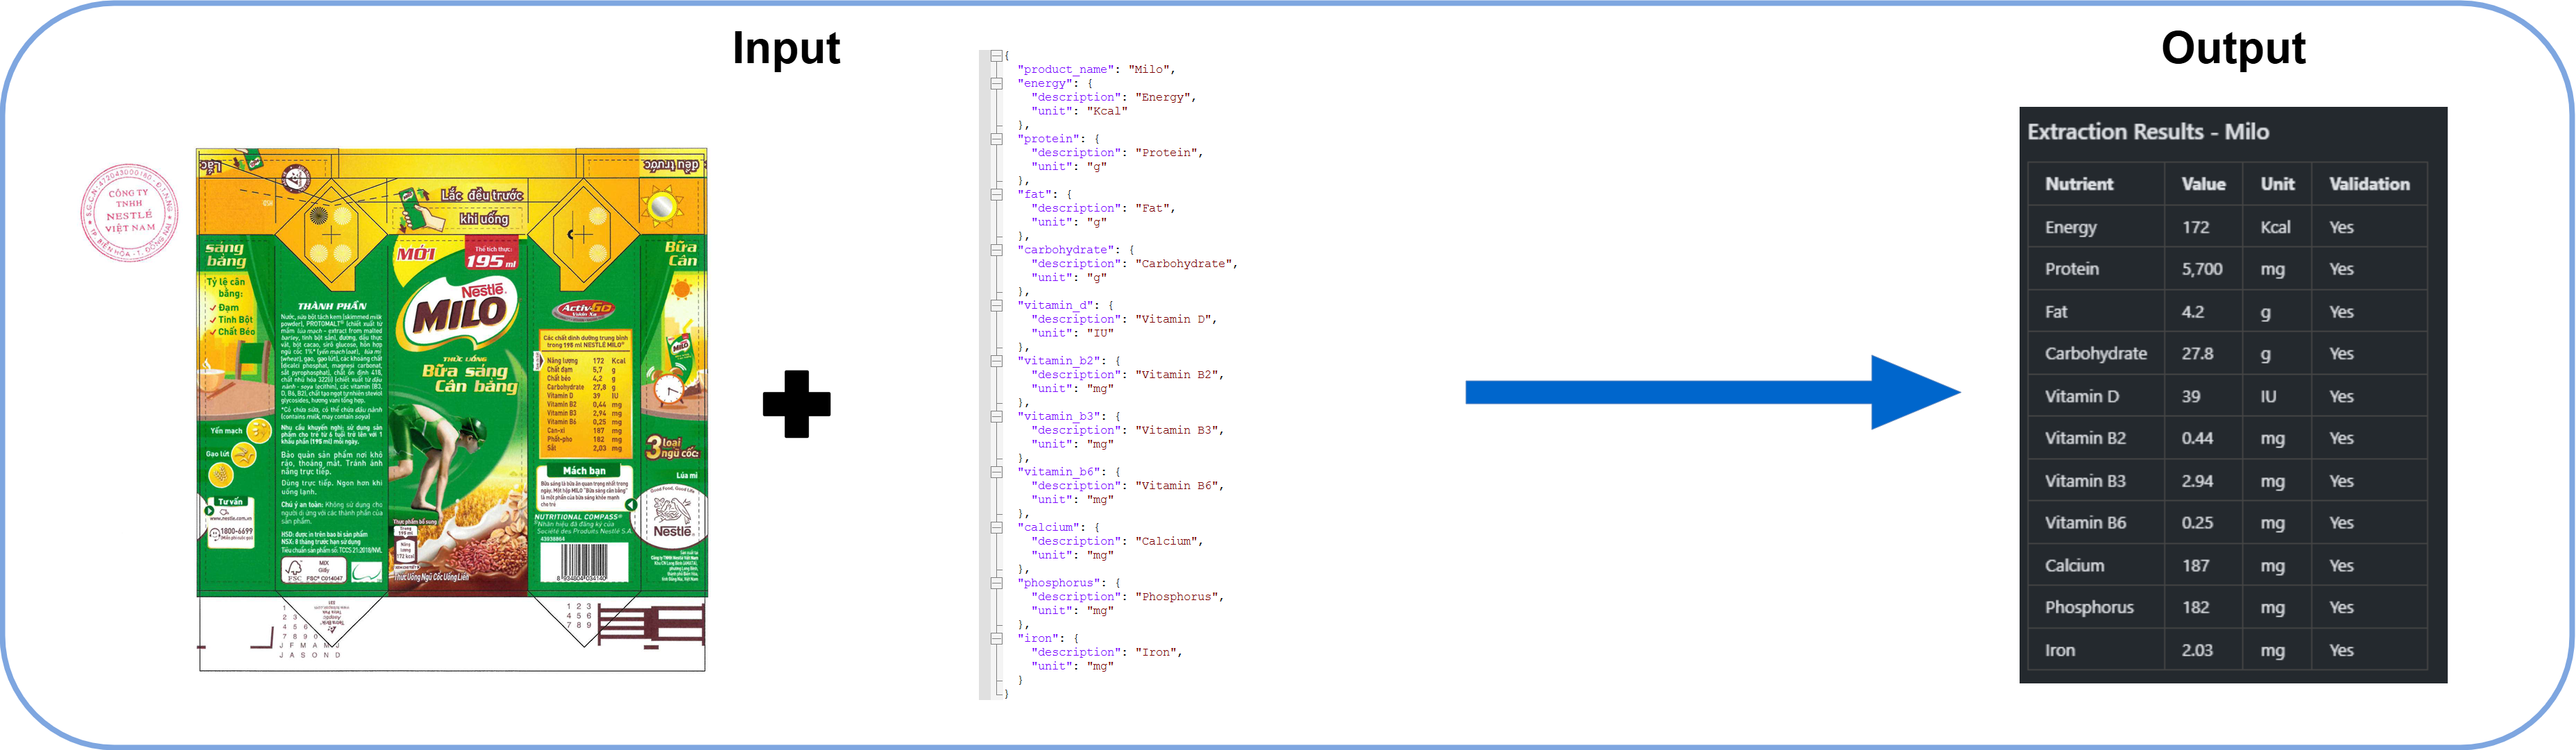
\includegraphics[width=\linewidth]{Images/Thesis_Solutions-Overall.png}
    \caption{Minh họa bài toán trích xuất dữ liệu có cấu trúc}
    \label{fig:sde_overview}
\end{figure}

Qua khảo sát tài liệu hiện có \cite{berghaus2025invoice,yashwant2025invoice,cheng2026hybrid,jin2025multistage}, tôi nhận thấy chưa có nghiên cứu nào đồng thời thỏa mãn ba điều kiện: (1) xử lý tài liệu tiếng Việt; (2) so sánh trực tiếp VLM và OCR-LLM trên cùng một framework đánh giá chuẩn hóa; và (3) phân tích riêng biệt giữa văn bản đánh máy (typed) và viết tay (handwritten). Nhận thấy khoảng trống này, tôi quyết định thực hiện đề tài nhằm lấp đầy cả ba điều kiện trên.

\section{Mục tiêu nghiên cứu}\label{sec:muctieu}

Đề tài theo đuổi hai mục tiêu song song:

\begin{enumerate}
    \item \textbf{Đánh giá và so sánh:} Xây dựng framework benchmark chuẩn hóa để đánh giá và so sánh toàn diện hai hướng tiếp cận VLM Direct Extraction và OCR-LLM Pipeline trên bốn chiều: độ chính xác (accuracy), độ bền vững (robustness), hiệu quả (efficiency) và độ tin cậy (reliability).

    \item \textbf{Xây dựng hệ thống:} Dựa trên kết quả thực nghiệm từ mục tiêu 1, thiết kế và hiện thực một hệ thống trích xuất dữ liệu có cấu trúc thực tế, có thể triển khai được trong môi trường sản xuất với các loại tài liệu invoice, CCCD và hợp đồng.
\end{enumerate}

\section{Phạm vi và giới hạn nghiên cứu}\label{sec:phamvi}

\noindent\textbf{Phạm vi nghiên cứu:}

\begin{table}[h]
\centering
\caption{Phạm vi nghiên cứu của đề tài}
\label{tab:phamvi}
\begin{tabular}{|l|p{9cm}|}
\hline
\textbf{Chiều} & \textbf{Giới hạn} \\ \hline
Loại tài liệu & Hóa đơn, Thẻ căn cước công dân (CCCD), Hợp đồng \\ \hline
Ngôn ngữ & Tiếng Anh (EN) và tiếng Việt (VI) \\ \hline
Dạng văn bản & Văn bản đánh máy và viết tay \\ \hline
Nguồn dữ liệu & Tập dữ liệu công khai; tài liệu thực tế tác giả tự thu thập \\ \hline
Output & JSON có cấu trúc theo schema định trước \\ \hline
\end{tabular}
\end{table}

\bigskip

\noindent\textbf{Giới hạn nghiên cứu:}

\begin{itemize}
    \item Không đánh giá trên tài liệu nhiều trang (multi-page) hoặc tài liệu PDF phức tạp có bảng biểu lồng nhau.
    \item Các mô hình VLM được đánh giá theo chế độ zero-shot; không thực hiện fine-tuning do giới hạn về tài nguyên tính toán.
    \item Dữ liệu tiếng Việt được thu thập từ tài liệu ngân hàng thực và nguồn thực tế; chi tiết được trình bày tại \hyperref[sec:datasets]{Mục 4.2}.
    \item Đánh giá hiệu quả chi phí dựa trên mức giá API tại thời điểm thực nghiệm; có thể thay đổi theo thời gian.
\end{itemize}

\section{Đóng góp của luận văn}\label{sec:donggop}

Luận văn có bốn đóng góp chính:

\begin{enumerate}
    \item \textbf{Framework đánh giá chuẩn hóa:} Xây dựng bộ tiêu chí và quy trình đánh giá thống nhất cho bài toán trích xuất dữ liệu có cấu trúc từ tài liệu, bao gồm bốn chiều accuracy, robustness, efficiency và reliability với các metric cụ thể.

    \item \textbf{Bộ kết quả benchmark toàn diện:} Cung cấp kết quả so sánh định lượng giữa VLM Direct Extraction và OCR-LLM Pipeline trên nhiều mô hình, nhiều loại tài liệu và hai ngôn ngữ Anh--Việt. Đây là benchmark đầu tiên có sự phân tích riêng biệt typed vs.\ handwritten cho tiếng Việt.

    \item \textbf{Phân tích khoảng trống ngôn ngữ Việt:} Đánh giá mức độ sụt giảm hiệu năng khi chuyển từ tài liệu tiếng Anh sang tiếng Việt, cung cấp bằng chứng thực nghiệm cho cộng đồng nghiên cứu NLP tiếng Việt.

    \item \textbf{Hệ thống trích xuất thực tế:} Thiết kế và hiện thực một hệ thống hoàn chỉnh có khả năng triển khai, tích hợp pipeline tốt nhất được xác định qua thực nghiệm.
\end{enumerate}

\section{Tổng quan về báo cáo}\label{sec:tongquan}

Luận văn được tổ chức thành 5 chương như sau:

\begin{itemize}
    \item \textbf{Chương 1 -- Giới thiệu:} Giới thiệu tổng quan về bối cảnh, mục tiêu, phạm vi, đóng góp của đề tài và cấu trúc của luận văn.
    \item \textbf{Chương 2 -- Công trình liên quan:} Khảo sát các nghiên cứu hiện có về hai hướng tiếp cận OCR-LLM và VLM. Từ đó xác định khoảng trống nghiên cứu mà đề tài hướng đến lấp đầy.
    \item \textbf{Chương 3 -- Cơ sở lý thuyết:} Trình bày nền tảng lý thuyết về IDP, OCR, LLM, VLM, bài toán trích xuất dữ liệu có cấu trúc và các chỉ số đánh giá được sử dụng trong thực nghiệm.
    \item \textbf{Chương 4 -- Phương pháp đề xuất:} Mô tả kiến trúc tổng thể, dữ liệu thực nghiệm, thiết kế hai pipeline, kết quả benchmark và thiết kế hệ thống cuối.
    \item \textbf{Chương 5 -- Kết luận:} Tổng kết kết quả, nhận xét hạn chế và đề xuất hướng phát triển trong tương lai.
\end{itemize}

\clearpage

% ============================================================
% CHƯƠNG 2 — CÔNG TRÌNH LIÊN QUAN
% ============================================================
\chapter{Công trình liên quan}

Trong chương này, tác giả sẽ trình bày các công trình nghiên cứu tiêu biểu liên quan đến bài toán trích xuất dữ liệu có cấu trúc từ tài liệu, tập trung vào hai hướng tiếp cận chính: VLM trực tiếp và pipeline OCR-LLM.

\section[Multi-Modal Vision vs.\ Text-Based Parsing]{Multi-Modal Vision vs.\ Text-Based Parsing: Benchmarking LLM Strategies for Invoice Processing}\label{sec:rw_berghaus}

Berghaus và cộng sự \cite{berghaus2025invoice} thực hiện nghiên cứu benchmark toàn diện so sánh hiệu năng hai chiến lược xử lý tài liệu invoice: đưa ảnh trực tiếp vào mô hình ngôn ngữ thị giác và chuyển đổi tài liệu sang văn bản có cấu trúc trước khi đưa vào LLM. Nghiên cứu đánh giá 8 mô hình đa phương thức với zero-shot prompting trên 3 tập dữ liệu invoice công khai, so sánh hai chiến lược:
\begin{itemize}
    \item \textbf{VLM Direct:} Đưa ảnh tài liệu trực tiếp vào model để sinh JSON output.
    \item \textbf{Text-Based (OCR-LLM):} Chuyển PDF sang Markdown bằng Docling, sau đó đưa text vào LLM để sinh JSON có cấu trúc.
\end{itemize}
Các model được benchmark bao gồm GPT-5, Gemini 2.5, Gemma 3 và 5 model khác, với field-level accuracy là metric đánh giá chính.

\paragraph{Nhận xét:}
Đây là công trình liên quan trực tiếp nhất với đề tài; cùng paradigm benchmark VLM vs OCR-LLM, cùng loại tài liệu invoice, cùng zero-shot setting. Đóng góp nổi bật là bộ kết quả so sánh định lượng trên nhiều model với cùng prompt template và cùng metric đánh giá, tạo tiền đề cho các nghiên cứu benchmark tiếp theo. Tuy nhiên, phạm vi thực nghiệm giới hạn ở tài liệu tiếng Anh, văn bản đánh máy, và chỉ một loại tài liệu.

\section[Invoice Information Extraction]{Invoice Information Extraction: Methods and Performance Evaluation}\label{sec:rw_yashwant}

Yashwant và cộng sự \cite{yashwant2025invoice} đề xuất một framework trích xuất thông tin từ invoice kết hợp công cụ phân tích tài liệu Docling và nền tảng LlamaCloud Services, đồng thời xây dựng bộ tiêu chí đánh giá chuẩn hóa cho bài toán này. Pipeline hoạt động theo hai bước: Docling phân tích cấu trúc tài liệu và trích xuất văn bản, sau đó LlamaCloud Services trích xuất các trường thông tin mục tiêu gồm invoice number, date, total amount và vendor details. Bộ tiêu chí đánh giá được đề xuất gồm field-level precision, consistency check failures và exact match accuracy.

\paragraph{Nhận xét:}
Đóng góp chính của nghiên cứu là bộ tiêu chí đánh giá chuẩn hóa, cho phép so sánh công bằng giữa các phương pháp trích xuất khác nhau. Cách tiếp cận kết hợp Docling và LlamaCloud cho thấy tiềm năng của pipeline OCR-LLM trên tài liệu invoice tiếng Anh; tuy nhiên phạm vi đánh giá còn giới hạn ở một ngôn ngữ và một loại tài liệu.

\section[Hybrid Architecture for Claim Document Understanding]{A Hybrid Architecture for Multi-Stage Claim Document Understanding}\label{sec:rw_cheng}

Cheng và cộng sự \cite{cheng2026hybrid} đề xuất kiến trúc hybrid ba giai đoạn cho bài toán hiểu tài liệu yêu cầu bảo hiểm, đã được triển khai thực tế tại 9 thị trường Đông Nam Á và Đông Á bao gồm Việt Nam, Singapore, Philippines, Indonesia, Malaysia, Trung Quốc, Hong Kong, Papua New Guinea và Campuchia. Pipeline ba giai đoạn cố định gồm: (1)~PaddleOCR nhận dạng văn bản đa ngôn ngữ, (2)~Logistic Regression phân loại loại tài liệu, và (3)~Qwen2.5-VL-7B trích xuất field theo schema định sẵn dựa trên loại tài liệu đã xác định.

\paragraph{Nhận xét:}
Điểm mạnh của nghiên cứu là thiết kế pipeline phù hợp với môi trường đa ngôn ngữ bao gồm tiếng Việt, đạt độ trễ dưới 2 giây phù hợp cho xử lý thời gian thực. Kiến trúc phân giai đoạn PaddleOCR $\rightarrow$ phân loại $\rightarrow$ Qwen2.5-VL-7B cho thấy compact VLM có thể đạt hiệu năng cao khi được kết hợp với bước phân loại tài liệu trước. Tuy nhiên, nghiên cứu không đánh giá đối chiếu giữa VLM Direct và OCR-LLM nên không trả lời được câu hỏi hướng tiếp cận nào tổng quát tốt hơn.

\section[Multi-Stage Field Extraction with Compact VLMs]{Multi-Stage Field Extraction of Financial Documents with OCR and Compact Vision-Language Models}\label{sec:rw_jin}

Jin và cộng sự \cite{jin2025multistage} đề xuất pipeline đa giai đoạn kết hợp OCR truyền thống với compact VLM nhằm trích xuất field từ tài liệu tài chính đa ngôn ngữ, với trọng tâm tối ưu hóa chi phí GPU và độ trễ xử lý. Pipeline gồm bốn giai đoạn: (1)~tiền xử lý ảnh (phân đoạn, phát hiện hướng, chuẩn hóa kích thước), (2)~OCR đa ngôn ngữ, (3)~page retrieval phân loại và liên kết các trang liên quan, và (4)~compact VLM trích xuất field trong phạm vi trang đã xác định thay vì toàn bộ tài liệu.

\paragraph{Nhận xét:}
Nghiên cứu đóng góp kỹ thuật page retrieval như một bước trung gian hiệu quả trước khi đưa nội dung vào VLM, từ đó cải thiện đáng kể cả độ chính xác lẫn hiệu quả tính toán. Kết quả thực nghiệm cho thấy compact VLM với pipeline tiền xử lý phù hợp có thể vượt trội large VLM khi áp dụng trực tiếp trên toàn tài liệu, gợi mở hướng thiết kế thực tế cho hệ thống sản xuất có ràng buộc về chi phí.

\section[OmniAI OCR Benchmark]{OmniAI OCR Benchmark\protect\footnote{OmniAI OCR Benchmark: \url{https://getomni.ai/ocr-benchmark}}}\label{sec:rw_omniai}

OmniAI công bố bộ benchmark liên tục cập nhật so sánh hiệu năng giữa các nhà cung cấp OCR truyền thống và các mô hình ngôn ngữ thị giác trên 1.000 tài liệu thực tế. Quy trình đánh giá: Document $\rightarrow$ OCR/VLM $\rightarrow$ GPT-4o (judge) $\rightarrow$ so sánh JSON output với ground truth theo JSON field-level differences, thay vì edit distance trên text thô. Các hệ thống được test bao gồm Traditional OCR (Azure Document Intelligence, AWS Textract, Google Document AI) và VLM (OpenAI, Gemini, Anthropic). Metrics: accuracy (tỷ lệ JSON field chính xác), cost (USD/1.000 trang), latency (giây/trang).

\paragraph{Nhận xét:}
OmniAI Benchmark đóng góp methodology đánh giá thực tế hướng đến ứng dụng sản xuất, với ba chiều accuracy--cost--latency phủ phần lớn yêu cầu của hệ thống trích xuất thực tế. Phương pháp dùng GPT-4o làm judge và so sánh JSON differences là cách tiếp cận phù hợp hơn cho bài toán structured extraction so với các metric dựa trên edit distance. Tuy nhiên, dataset chủ yếu tiếng Anh và không có phân tích riêng theo typed vs. handwritten.

\section{Tổng hợp và xác định khoảng trống nghiên cứu}\label{sec:research_gap}

Qua khảo sát các công trình tiêu biểu, có thể nhận thấy rằng mỗi nghiên cứu chỉ đáp ứng một hoặc hai trong số các điều kiện đặt ra. Bảng~\ref{tab:research_gap} tổng hợp mức độ đáp ứng của từng công trình theo các chiều so sánh chính.

\begin{table}[h]
\centering
\caption{So sánh các công trình liên quan và khoảng trống nghiên cứu}
\label{tab:research_gap}
\footnotesize
\renewcommand{\arraystretch}{1.3}
\begin{tabular}{|p{4cm}|p{1.7cm}|p{2.1cm}|p{2cm}|p{2.2cm}|p{2.4cm}|}
\hline
\textbf{Công trình} & \textbf{Tiếng Việt} & \textbf{So sánh VLM vs OCR-LLM} & \textbf{Đánh máy + Viết tay} & \textbf{Đa dạng tài liệu} & \textbf{Đánh giá 4 chiều} \\ \hline
Multi-Modal Vision vs. Text-Based Parsing: Benchmarking LLM Strategies for Invoice Processing & $\times$ & $\checkmark$ & $\times$ & $\times$ & $\times$ \\ \hline
Invoice Information Extraction: Methods and Performance Evaluation & $\times$ & Chỉ OCR-LLM, không so sánh & $\times$ & $\times$ & $\times$ \\ \hline
A Hybrid Architecture for Multi-Stage Claim Document Understanding & VN là 1 trong 9 thị trường & $\times$ & Tài liệu bảo hiểm thực tế, chưa phân tích riêng & $\times$ & $\times$ \\ \hline
Multi-Stage Field Extraction of Financial Documents with OCR and Compact Vision-Language Models & $\times$ & $\times$ & $\times$ & $\times$ & Chỉ accuracy + efficiency, thiếu robustness và reliability \\ \hline
OmniAI OCR Benchmark & $\times$ & $\checkmark$ & $\times$ & Tài liệu thực tế hỗn hợp, không phân loại rõ & Chỉ accuracy + cost + latency, thiếu reliability \\ \hline
\rowcolor{yellow!25}
\textbf{Đề tài} & \textbf{$\checkmark$} & \textbf{$\checkmark$} & \textbf{$\checkmark$} & \textbf{$\checkmark$} & \textbf{$\checkmark$} \\ \hline
\end{tabular}
\end{table}

Có thể nhận thấy rằng chưa có công trình nào đồng thời thỏa mãn: (1) xử lý tài liệu tiếng Việt; (2) so sánh trực tiếp VLM Direct và OCR-LLM Pipeline trên cùng framework đánh giá chuẩn hóa; và (3) phân tích riêng biệt hiệu năng trên văn bản đánh máy và viết tay. Nhận thấy khoảng trống này, đề tài được thiết kế nhằm lấp đầy đồng thời cả ba điều kiện trên, với phạm vi mở rộng sang ba loại tài liệu phổ biến trong nghiệp vụ doanh nghiệp: hóa đơn, thẻ căn cước công dân và hợp đồng.

\clearpage

% ============================================================
% CHƯƠNG 3 — CƠ SỞ LÝ THUYẾT
% ============================================================
\chapter{Cơ sở lý thuyết}

Trong chương này, tác giả sẽ trình bày các kiến thức nền tảng cần thiết để hướng đến việc xây dựng hệ thống trích xuất dữ liệu có cấu trúc từ đa dạng tài liệu, bao gồm tổng quan về xử lý tài liệu thông minh, các công nghệ nhận dạng ký tự quang học, mô hình ngôn ngữ lớn, mô hình ngôn ngữ thị giác, kỹ thuật trích xuất dữ liệu có cấu trúc, và các chỉ số đánh giá được sử dụng trong thực nghiệm.

\section{Tổng quan về trích xuất dữ liệu từ tài liệu thông minh (IDP)}\label{sec:idp}

\begin{quote}
\emph{``Intelligent Document Processing (IDP) is a domain that is part of the challenge of information digitalization constituting the Industrial Revolution of the twenty-first century (Industry 4.0), specifically focused on the difficult areas of classifying, extracting information from, and integrating into business processes documents such as forms and invoices.''} \cite{zhu2021idp}
\end{quote}

Có thể hiểu rằng xử lý tài liệu thông minh (Intelligent Document Processing - IDP) là lĩnh vực ứng dụng trí tuệ nhân tạo nhằm tự động hóa quá trình phân loại, trích xuất và tích hợp thông tin từ các tài liệu dưới dạng số hóa vào các quy trình nghiệp vụ. Đây được xem là một phần cốt lõi của làn sóng chuyển đổi số trong bối cảnh Cách mạng Công nghiệp 4.0, đặc biệt tập trung vào hai thách thức khó nhất là phân loại tài liệu và trích xuất thông tin từ hóa đơn, biểu mẫu và hợp đồng.

Hệ thống IDP hiện đại tích hợp nhiều công nghệ khác nhau, bao gồm OCR, xử lý ngôn ngữ tự nhiên (Natural Language Processing - NLP), học máy (Machine Learning - ML) và thị giác máy tính (Computer Vision). Sự kết hợp này cho phép hệ thống xử lý không chỉ văn bản thuần túy mà còn cả bố cục, hình ảnh, bảng biểu và các yếu tố trực quan khác trong tài liệu.

Tài liệu đầu vào trong hệ thống IDP thường thuộc một trong ba dạng chính:

\begin{itemize}
    \item \textbf{Tài liệu có cấu trúc} (structured documents): các biểu mẫu có bố cục cố định, ví dụ tờ khai thuế hay phiếu xuất kho, trong đó thông tin luôn xuất hiện ở vị trí xác định trước.
    \item \textbf{Tài liệu bán cấu trúc} (semi-structured documents): các hóa đơn thương mại hay chứng minh nhân dân, trong đó tồn tại một cấu trúc ngữ nghĩa nhất định nhưng bố cục trực quan thay đổi tùy nhà phát hành.
    \item \textbf{Tài liệu phi cấu trúc} (unstructured documents): hợp đồng, báo cáo, thư từ, trong đó thông tin được nhúng trong văn bản tự do không theo khuôn mẫu cố định.
\end{itemize}

Trong phạm vi đề tài này, tác giả tập trung vào dạng tài liệu bán cấu trúc và phi cấu trúc, cụ thể là hóa đơn, căn cước công dân và hợp đồng. Đây là ba loại tài liệu phổ biến trong các quy trình nghiệp vụ thực tế tại Việt Nam.

Quy trình xử lý tổng quát trong một hệ thống IDP bao gồm năm giai đoạn kế tiếp nhau, được minh họa tại Hình~\ref{fig:idp_pipeline}:

\begin{enumerate}
    \item \textbf{Thu nhận tài liệu} (Document Capture): tiếp nhận tài liệu đầu vào ở các định dạng khác nhau như PDF, ảnh chụp hoặc ảnh scan, và chuẩn bị cho các bước xử lý tiếp theo.
    \item \textbf{Tiền xử lý} (Pre-processing): chuẩn hóa chất lượng ảnh, xoay chỉnh, khử nhiễu nhằm cải thiện đầu vào và tăng độ chính xác cho các giai đoạn sau.
    \item \textbf{Phân loại tài liệu} (Classification): xác định loại tài liệu (hóa đơn, hợp đồng, biểu mẫu, ...) để áp dụng schema trích xuất phù hợp trong bước tiếp theo.
    \item \textbf{Trích xuất dữ liệu} (Data Extraction): nhận dạng và trích xuất các trường thông tin có giá trị nghiệp vụ từ tài liệu, tạo ra đầu ra dạng có cấu trúc.
    \item \textbf{Xác thực dữ liệu} (Data Validation): kiểm tra tính hợp lệ của dữ liệu trích xuất theo schema định sẵn, gắn cờ các trường có độ tin cậy thấp hoặc thiếu giá trị trước khi tích hợp vào hệ thống nghiệp vụ.
\end{enumerate}

\begin{figure}[H]
    \centering
    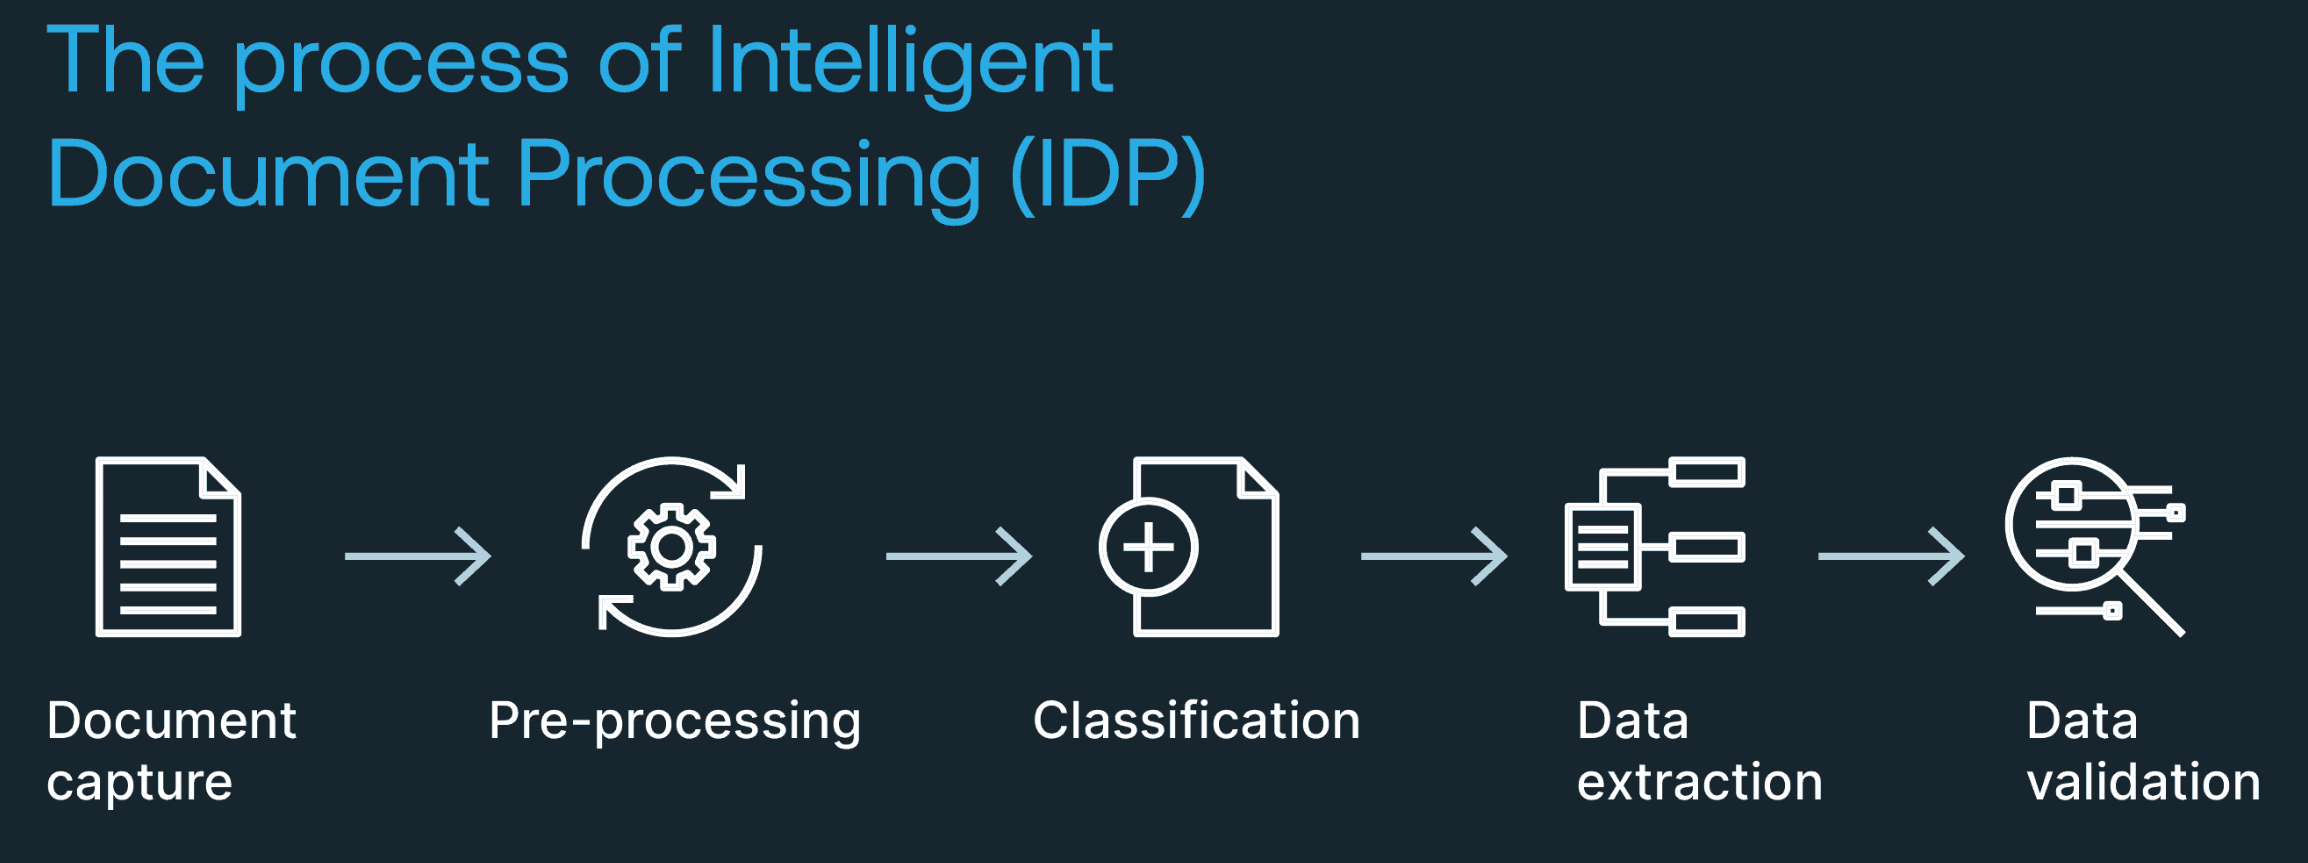
\includegraphics[width=0.85\linewidth]{Images/IDP-Workflow-Overall.png}
    \caption{Quy trình tổng quát của hệ thống Xử lý Tài liệu Thông minh (IDP)}
    \label{fig:idp_pipeline}
\end{figure}

Có thể nhận thấy rằng giai đoạn trích xuất dữ liệu là trọng tâm của toàn bộ hệ thống IDP, và cũng là điểm khác biệt chính giữa hai hướng tiếp cận mà đề tài này nghiên cứu: \hyperref[sec:vlm_pipeline]{VLM Direct Extraction} và \hyperref[sec:ocr_llm_pipeline]{OCR-LLM Pipeline}.

\section{Optical Character Recognition (OCR)}\label{sec:ocr}

\begin{quote}
\emph{``Optical Character Recognition (OCR) refers to the conversion of images of typed, handwritten, or printed text into machine-encoded text, typically structured as a two-stage pipeline of text detection followed by text recognition.''} \cite{li2021trocr}
\end{quote}

OCR là công nghệ chuyển đổi hình ảnh chứa văn bản, dù là văn bản in ấn hay viết tay, thành dạng văn bản có thể xử lý bằng máy tính. Đây là một bài toán thị giác máy tính lâu đời, song vẫn là thành phần không thể thiếu trong hầu hết các hệ thống xử lý tài liệu hiện đại.

\subsection{Kiến trúc tổng quát}\label{sec:ocr_architecture}

Một hệ thống OCR hiện đại thường được chia thành hai giai đoạn chính:

\begin{itemize}
    \item \textbf{Phát hiện văn bản} (Text Detection): xác định và khoanh vùng các đoạn văn bản trong ảnh. Các phương pháp phổ biến gồm EAST, DBNet, và các biến thể dựa trên Feature Pyramid Network (FPN). Đầu ra là các bounding box hoặc polygon bao quanh từng dòng/từ văn bản.
    \item \textbf{Nhận dạng văn bản} (Text Recognition): giải mã nội dung bên trong vùng văn bản đã phát hiện. Kiến trúc truyền thống kết hợp mạng tích chập (Convolutional Neural Network - CNN) để trích xuất đặc trưng trực quan với mạng hồi tiếp (LSTM/GRU) để mô hình hóa chuỗi ký tự, sử dụng hàm mất mát CTC (Connectionist Temporal Classification) trong quá trình huấn luyện. Tuy nhiên, các kiến trúc hiện đại đã chuyển sang dùng Transformer thuần túy cho cả hai thành phần: điển hình là SVTR (Simple Visual Text Recognition) \cite{paddleocr2022}, thay thế hoàn toàn CRNN bằng một Transformer đơn khối xử lý đặc trưng thị giác theo cơ chế self-attention, đạt độ chính xác và tốc độ suy luận vượt trội so với kiến trúc CNN-LSTM. Trong PP-OCRv3 \cite{paddleocr2022}, SVTR được tích hợp làm backbone nhận dạng chính, kết hợp với các kỹ thuật data augmentation và knowledge distillation để tối ưu cho triển khai thực tế, như minh họa ở Hình~\ref{fig:ocr_pipeline}.
\end{itemize}

\begin{figure}[H]
    \centering
    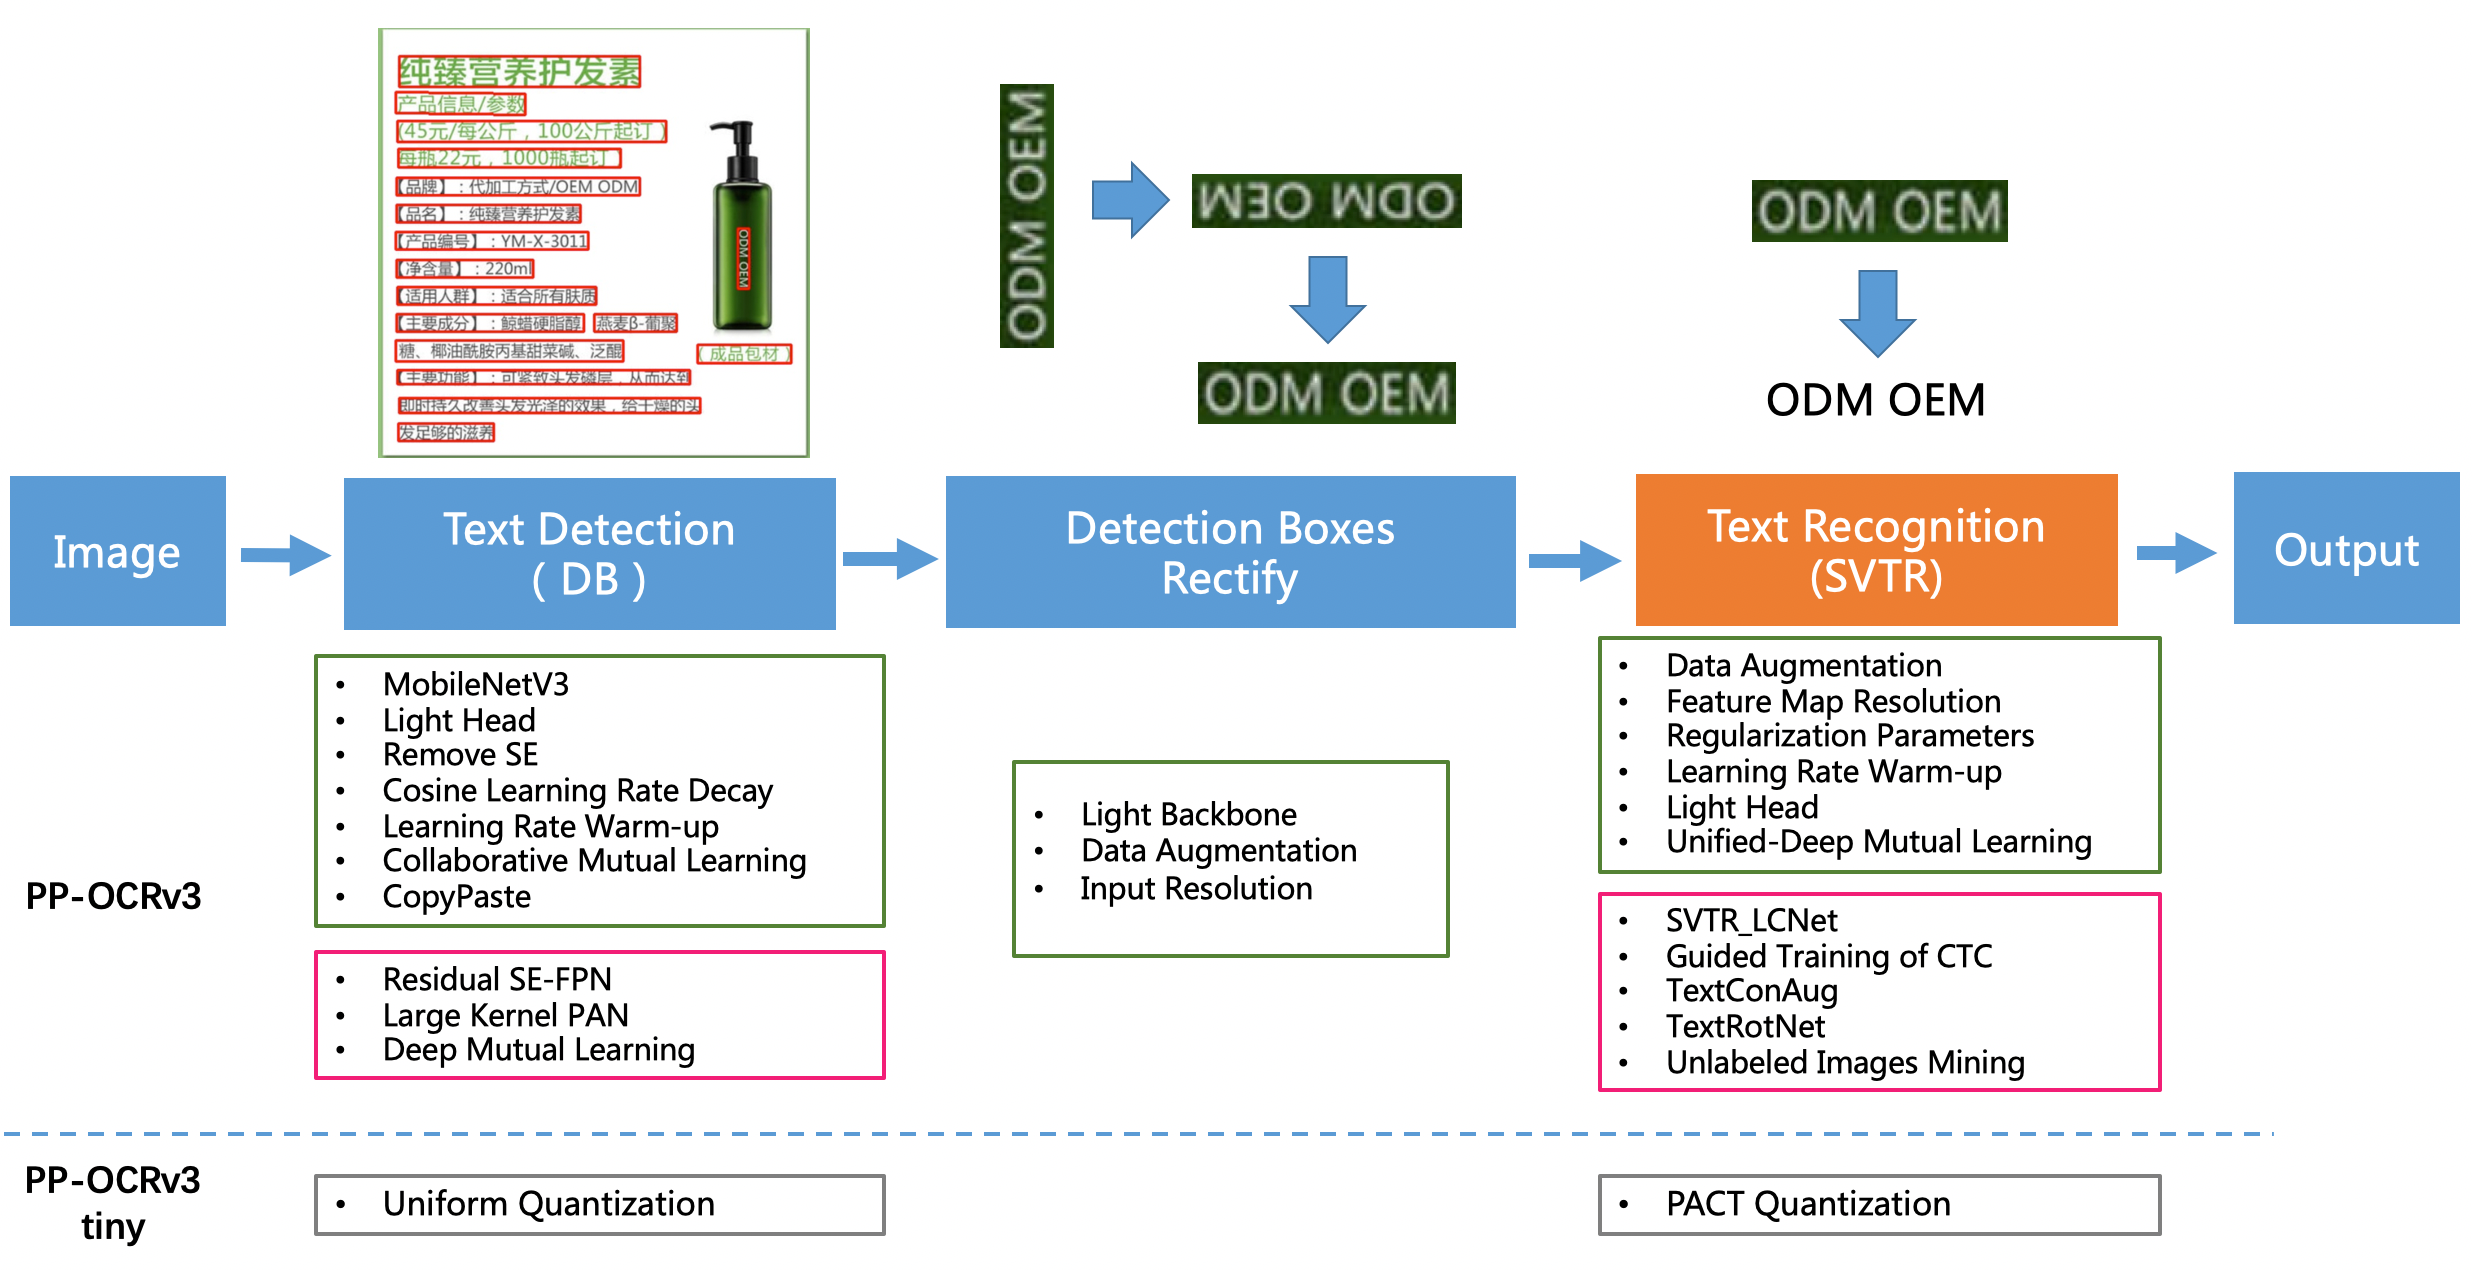
\includegraphics[width=0.9\linewidth]{Images/3_2_ocr_pipeline.png}
    \caption{Kiến trúc hệ thống nhận dạng văn bản PP-OCRv3 \cite{paddleocr2022}}
    \label{fig:ocr_pipeline}
\end{figure}

\subsection{Các công cụ OCR được sử dụng trong đề tài}\label{sec:ocr_tools}

Đề tài sử dụng hai công cụ OCR đại diện cho hai hướng tiếp cận khác nhau: một thư viện mã nguồn mở chạy cục bộ và một dịch vụ đám mây thương mại.

\textbf{EasyOCR}\footnote{EasyOCR: \url{https://github.com/JaidedAI/EasyOCR}} là thư viện OCR mã nguồn mở, hỗ trợ hơn 80 ngôn ngữ bao gồm tiếng Việt. Công cụ này theo kiến trúc hai giai đoạn với mô hình phát hiện văn bản CRAFT và mô hình nhận dạng CRNN, có thể chạy trên cả CPU lẫn GPU mà không phụ thuộc dịch vụ bên ngoài. EasyOCR được chọn làm OCR engine mặc định cho \hyperref[sec:ocr_llm_pipeline]{OCR-LLM Pipeline} nhờ chi phí bằng không, dễ triển khai và hỗ trợ tiếng Việt sẵn có.

\textbf{Azure AI Document Intelligence}\footnotemark{} là dịch vụ OCR thương mại của Microsoft, được cung cấp dưới dạng API trên nền tảng Azure. Dịch vụ này tích hợp sẵn các mô hình phân tích bố cục tài liệu phức tạp, hỗ trợ trích xuất văn bản, bảng biểu và các trường có cấu trúc từ nhiều loại tài liệu khác nhau. Trong đề tài, tác giả sử dụng pre-built model \texttt{prebuilt-read} để trích xuất văn bản theo đúng thứ tự đọc, đại diện cho hướng OCR đám mây chất lượng cao để đối chiếu với EasyOCR.
\footnotetext{Azure AI Document Intelligence: \url{https://learn.microsoft.com/azure/ai-services/document-intelligence/}}

\subsection{Thách thức của OCR trong bài toán trích xuất tài liệu}\label{sec:ocr_challenges}

Hiệu năng OCR ảnh hưởng trực tiếp đến chất lượng đầu vào của toàn bộ \hyperref[sec:ocr_llm_pipeline]{OCR-LLM Pipeline}. Các thách thức chính bao gồm:

\begin{itemize}
    \item \textbf{Chất lượng ảnh thấp}: ảnh mờ, nghiêng, ánh sáng không đều làm giảm độ chính xác nhận dạng.
    \item \textbf{Văn bản viết tay}: độ chính xác thấp hơn đáng kể so với văn bản đánh máy, đặc biệt với chữ viết tay tiếng Việt có dấu thanh.
    \item \textbf{Mất thông tin bố cục}: OCR truyền thống chỉ trả về chuỗi văn bản phẳng, làm mất thông tin về vị trí tương đối giữa các trường, vốn là thông tin quan trọng trong hóa đơn và biểu mẫu.
\end{itemize}

Chính hạn chế cuối cùng này là một trong những lý do thúc đẩy hướng tiếp cận \hyperref[sec:vlm_pipeline]{VLM Direct Extraction}, khi mô hình có thể nhìn trực tiếp vào ảnh tài liệu và tự hiểu bố cục mà không phụ thuộc vào bước OCR trung gian.

\section{Large Language Model (LLM)}\label{sec:llm}

\begin{quote}
\emph{``Large Language Models (LLMs) are deep neural networks with billions of parameters, pre-trained on massive text corpora using self-supervised objectives, capable of natural language understanding, generation, and reasoning at near-human levels on many tasks.''} \cite{openai2023gpt4}
\end{quote}

LLM là các mô hình ngôn ngữ học sâu có quy mô tham số lớn, có khả năng hiểu, tạo sinh và suy luận trên ngôn ngữ tự nhiên ở mức độ tiệm cận năng lực con người trên nhiều tác vụ thực tế. Sức mạnh của LLM bắt nguồn từ kiến trúc Transformer kết hợp với chiến lược pre-training trên dữ liệu web-scale.

\subsection{Kiến trúc Transformer}\label{sec:transformer}

Nền tảng của mọi LLM hiện đại là kiến trúc Transformer, được Vaswani và cộng sự \cite{vaswani2017attention} giới thiệu năm 2017 trong bài báo ``Attention Is All You Need''. Transformer từ bỏ hoàn toàn cấu trúc hồi tiếp (Recurrent Neural Network - RNN) và thay bằng cơ chế self-attention, cho phép mô hình học mối quan hệ giữa bất kỳ hai vị trí nào trong chuỗi đầu vào chỉ trong một bước tính toán song song.

Cơ chế \textbf{Multi-Head Attention} là thành phần cốt lõi, được tính toán như sau:

\begin{equation}
    \text{Attention}(Q, K, V) = \text{softmax}\left(\frac{QK^\top}{\sqrt{d_k}}\right)V
\end{equation}

Trong đó:
\begin{itemize}
    \item $Q$, $K$, $V$: ma trận Query, Key, Value được chiếu tuyến tính từ đầu vào,
    \item $d_k$: chiều của vector Key, dùng để chuẩn hóa tránh vanishing gradient khi $d_k$ lớn.
\end{itemize}

Với Multi-Head Attention, phép tính này được thực hiện song song trên $h$ ``đầu'' khác nhau, cho phép mô hình chú ý đến thông tin từ nhiều không gian biểu diễn khác nhau đồng thời, như minh họa ở Hình~\ref{fig:transformer}.

\begin{figure}[H]
    \centering
    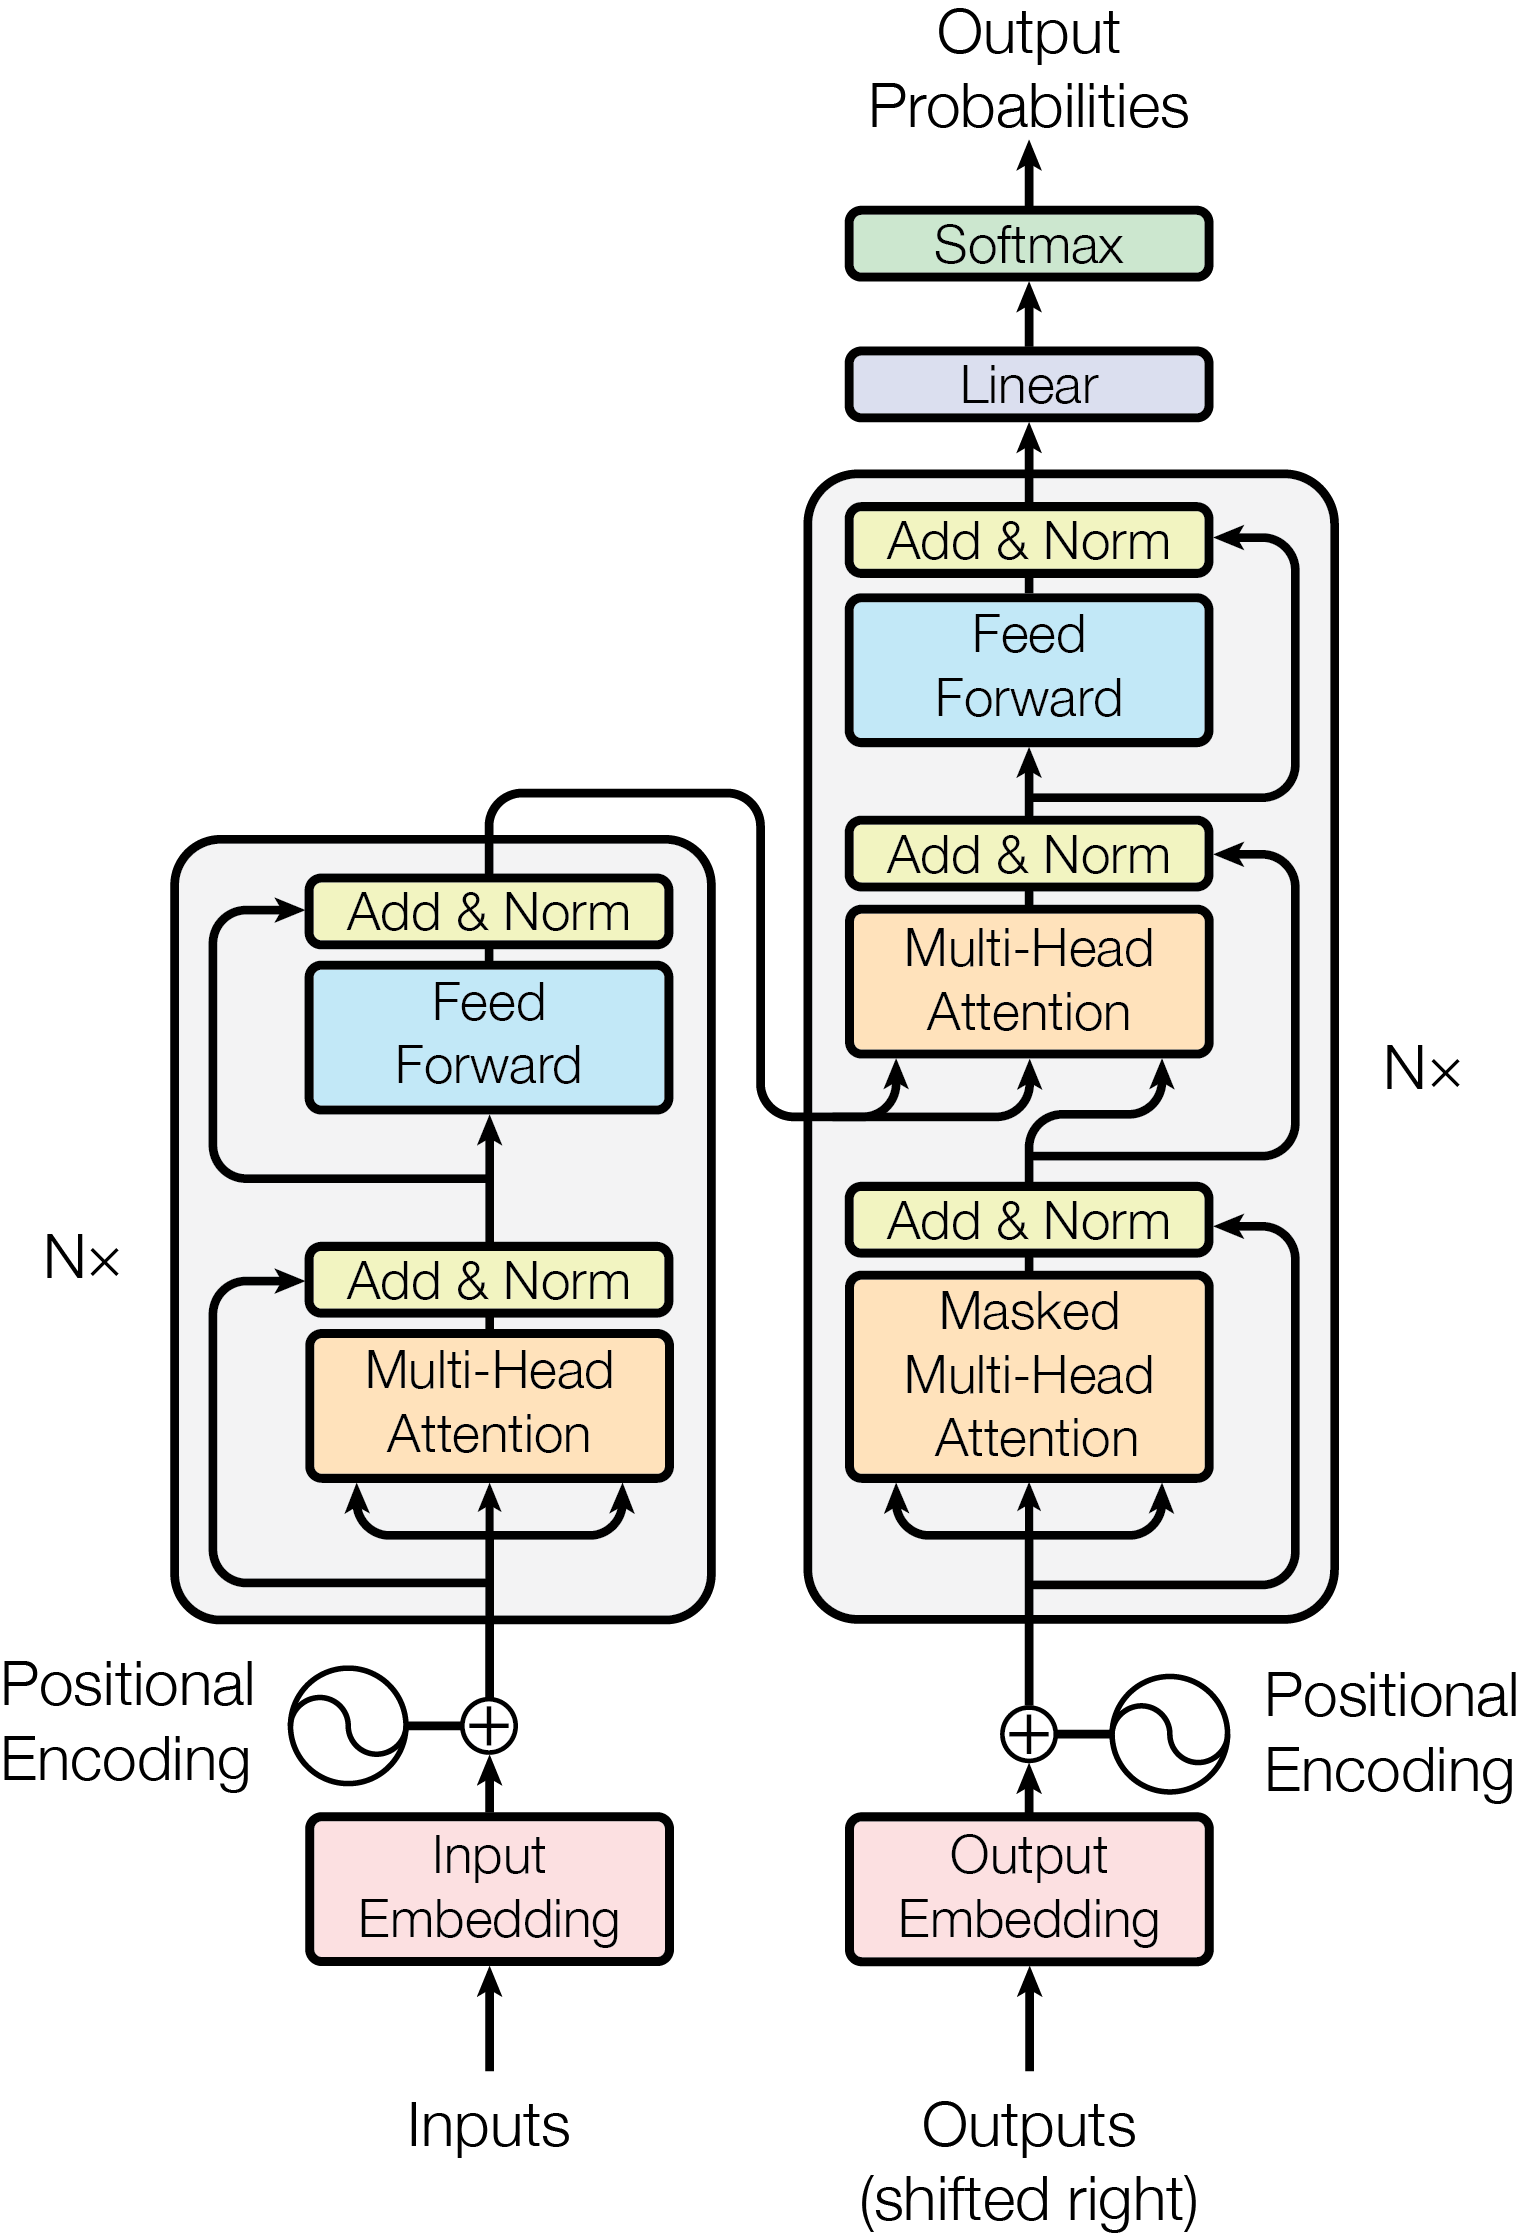
\includegraphics[width=0.55\linewidth]{Images/3_3_transformer.png}
    \caption{Kiến trúc Transformer gốc với Encoder (trái) và Decoder (phải) \cite{vaswani2017attention}}
    \label{fig:transformer}
\end{figure}

\subsection{Quá trình pre-training và fine-tuning}\label{sec:llm_training}

LLM hiện đại theo kiến trúc decoder-only (GPT-style) \cite{openai2023gpt4} được pre-train theo mục tiêu \textbf{causal language modeling}: dự đoán token tiếp theo dựa trên tất cả token trước đó. Quá trình này trên tập dữ liệu web-scale giúp mô hình học ngầm cấu trúc ngôn ngữ, tri thức thực tế và kỹ năng suy luận.

Sau giai đoạn pre-training, các kỹ thuật alignment được áp dụng để tinh chỉnh hành vi mô hình theo mục tiêu cụ thể:

\begin{itemize}
    \item \textbf{Instruction Tuning} (Supervised Fine-Tuning - SFT): fine-tune trên các cặp (instruction, response) chất lượng cao để mô hình tuân theo hướng dẫn của người dùng.
    \item \textbf{RLHF} (Reinforcement Learning from Human Feedback): tối ưu theo phản hồi người đánh giá nhằm cải thiện tính hữu ích và an toàn.
\end{itemize}

\subsection{Vai trò của LLM trong OCR-LLM Pipeline}\label{sec:llm_role}

Trong \hyperref[sec:ocr_llm_pipeline]{OCR-LLM Pipeline} của đề tài, LLM đóng vai trò là bộ phân tích ngữ nghĩa (semantic parser): nhận văn bản thô từ OCR đầu ra, hiểu ngữ nghĩa và ngữ cảnh, sau đó ánh xạ các giá trị về đúng trường trong JSON schema định sẵn. Nhiệm vụ này yêu cầu LLM có khả năng:

\begin{itemize}
    \item Xác định ranh giới giữa các trường thông tin không được phân tách rõ ràng.
    \item Chuẩn hóa định dạng (ngày tháng, tiền tệ, địa chỉ) về dạng thống nhất.
    \item Xử lý văn bản OCR có nhiễu với lỗi ký tự, thiếu dấu câu, hoặc sai chính tả.
    \item Tuân thủ nghiêm ngặt schema JSON đầu ra mà không tự thêm hoặc bỏ bất kỳ trường nào.
\end{itemize}

Năm mô hình đóng vai trò LLM trong \hyperref[sec:ocr_llm_pipeline]{OCR-LLM Pipeline}. Bốn trong số đó là các mô hình đa phương thức đồng thời được dùng làm VLM (GPT-4o, GPT-5.2-chat, Llama-4-Maverick-17B-128E-Instruct-FP8, Phi-4-multimodal-instruct), nhưng khi vận hành trong pipeline này chúng chỉ nhận đầu vào văn bản thuần từ OCR. Mô hình thứ năm là \textbf{DeepSeek-V4-Flash}\footnote{DeepSeek API: \url{https://api-docs.deepseek.com/}} của DeepSeek, một LLM thuần văn bản không hỗ trợ đầu vào hình ảnh, nên chỉ tham gia OCR-LLM Pipeline mà không xuất hiện trong VLM Direct Pipeline. Việc dùng chung bốn mô hình cho cả hai vai trò (VLM và LLM) là thiết kế thực nghiệm có chủ đích, nhằm cô lập và đo lường tác động của bước OCR tiền xử lý lên cùng một mô hình nền.

\section{Vision Language Model (VLM)}\label{sec:vlm}

\begin{quote}
\emph{``Vision Language Models (VLMs) integrate computer vision and natural language processing in a unified framework, enabling models to perform multimodal tasks that require simultaneous understanding of visual content and natural language semantics.''} \cite{vlmsurvey2025}
\end{quote}

VLM là lớp mô hình đa phương thức (multimodal) kết hợp khả năng hiểu hình ảnh của thị giác máy tính với khả năng suy luận ngôn ngữ của LLM, cho phép thực hiện các tác vụ đòi hỏi hiểu đồng thời cả nội dung trực quan và ngữ nghĩa ngôn ngữ. Đây là nền tảng kỹ thuật của hướng tiếp cận \hyperref[sec:vlm_pipeline]{VLM Direct Extraction} trong đề tài.

\subsection{Kiến trúc tổng quát}\label{sec:vlm_architecture}

Hầu hết các VLM hiện đại theo kiến trúc ba thành phần:

\begin{itemize}
    \item \textbf{Vision Encoder}: một Vision Transformer (ViT) hoặc CLIP encoder, chịu trách nhiệm mã hóa ảnh đầu vào thành chuỗi vector đặc trưng (image tokens/patch embeddings). Mỗi patch ảnh được chiếu thành một vector có chiều tương đương với embedding của LLM.
    \item \textbf{Projection Layer} (hay còn gọi là Connector/Adapter): một lớp tuyến tính hoặc Multi-Layer Perceptron (MLP) thu hẹp không gian biểu diễn từ vision encoder về không gian token của LLM, đảm bảo hai modality có thể ``nói chuyện'' với nhau trong cùng một không gian nhúng.
    \item \textbf{Language Decoder}: LLM backbone (thường là decoder-only transformer) nhận chuỗi gồm image tokens và text tokens, sau đó sinh ra phản hồi văn bản theo cơ chế autoregressive.
\end{itemize}

Luồng thông tin qua ba thành phần này có thể biểu diễn như sau: ảnh đầu vào $X_v$ được mã hóa bởi Vision Encoder thành vector đặc trưng $Z_v$; Projection Layer $W$ chiếu $Z_v$ về không gian biểu diễn của LLM để tạo ra image feature $H_v$; Language Model $f_\phi$ kết hợp $H_v$ với đặc trưng ngôn ngữ $H_q$ (trích xuất từ câu lệnh đầu vào $X_q$) rồi sinh ra phản hồi $X_a$. Kiến trúc ba thành phần này được giới thiệu trong LLaVA \cite{liu2023llava} và hiện là nền tảng của hầu hết các VLM hiện đại, như minh họa ở Hình~\ref{fig:vlm_architecture}.

\begin{figure}[H]
    \centering
    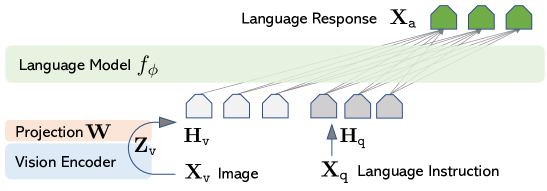
\includegraphics[width=0.88\linewidth]{Images/3_4_vlm_architecture.png}
    \caption{Kiến trúc tổng quát của Vision Language Model theo LLaVA \cite{liu2023llava}}
    \label{fig:vlm_architecture}
\end{figure}

\subsection{Các VLM được sử dụng trong đề tài}\label{sec:vlm_models_theory}

Đề tài đánh giá bốn mô hình VLM, đại diện cho cả hai luồng phát triển thương mại và mã nguồn mở, đều được truy cập qua nền tảng Azure.

\textbf{GPT-4o}\footnote{Azure OpenAI models: \url{https://learn.microsoft.com/azure/ai-services/openai/concepts/models}} của OpenAI thuộc dòng GPT-4 \cite{openai2023gpt4} là mô hình đa phương thức gốc (natively multimodal), xử lý hình ảnh và văn bản trong cùng một kiến trúc Transformer thống nhất. Trong đề tài, GPT-4o được sử dụng theo hai vai trò: vai VLM (nhận ảnh trực tiếp) trong \hyperref[sec:vlm_pipeline]{VLM Direct Extraction Pipeline}, và vai LLM thuần văn bản (nhận đầu vào từ OCR) trong \hyperref[sec:ocr_llm_pipeline]{OCR-LLM Pipeline}. Đây là thiết kế thực nghiệm có chủ đích nhằm đánh giá tác động của bước OCR tiền xử lý lên cùng một mô hình nền.

\textbf{GPT-5.2-chat} của OpenAI là mô hình đa phương thức thế hệ mới hơn trong dòng GPT, có năng lực suy luận và hiểu tài liệu được cải thiện. Cần lưu ý rằng mô hình này chỉ hỗ trợ giá trị temperature mặc định (bằng 1), khác với cấu hình temperature bằng 0 được áp dụng cho các mô hình còn lại nhằm đảm bảo tính tái lập.

\textbf{Llama-4-Maverick-17B-128E-Instruct-FP8}\footnote{Llama 4: \url{https://ai.meta.com/blog/llama-4-multimodal-intelligence/}} của Meta là VLM mã nguồn mở theo kiến trúc Mixture-of-Experts (MoE) với 17B tham số kích hoạt trên tổng 128 expert, hỗ trợ đa phương thức gốc. Phiên bản FP8 được lượng tử hóa nhằm giảm chi phí và tăng tốc độ suy luận.

\textbf{Phi-4-multimodal-instruct}\footnote{Phi-4-multimodal: \url{https://huggingface.co/microsoft/Phi-4-multimodal-instruct}} của Microsoft là VLM compact với khoảng 5.6B tham số, đại diện cho nhóm mô hình nhỏ gọn (small multimodal model). Do kích thước nhỏ, mô hình này phù hợp để khảo sát giới hạn năng lực của VLM compact trong bài toán trích xuất tài liệu.

\subsection{Nền tảng cung cấp mô hình: Azure AI Foundry}\label{sec:azure_foundry}

Toàn bộ các mô hình VLM và LLM trong đề tài được truy cập qua nền tảng đám mây của Microsoft thay vì tự host cục bộ, thông qua hai dịch vụ bổ trợ cho nhau:

\begin{itemize}
    \item \textbf{Azure OpenAI Service}: cung cấp các mô hình dòng GPT của OpenAI (GPT-4o, GPT-5.2-chat) dưới dạng deployment riêng, gọi qua REST API tương thích chuẩn OpenAI.
    \item \textbf{Azure AI Foundry} (tiền thân là Azure AI Studio): catalog mô hình hợp nhất cho phép triển khai mô hình nền từ nhiều nhà cung cấp (Meta Llama, Microsoft Phi, DeepSeek) qua một endpoint suy luận serverless chung, thanh toán theo lượng token (pay-as-you-go) mà không cần quản lý hạ tầng GPU.
\end{itemize}

Tác giả lựa chọn nền tảng này vì các đặc điểm sau:

\begin{itemize}
    \item \textbf{Truy cập thống nhất}: một khóa xác thực và một SDK duy nhất cho nhiều họ mô hình khác nhau, giúp việc benchmark nhiều mô hình trở nên nhất quán và dễ mở rộng.
    \item \textbf{Tính sẵn sàng và khả năng mở rộng}: hạ tầng suy luận do Microsoft quản lý, đảm bảo độ ổn định cao hơn so với các API miễn phí có hàng đợi vào giờ cao điểm.
    \item \textbf{Bảo mật dữ liệu}: tài liệu nhạy cảm như hóa đơn, hợp đồng và Căn cước công dân được xử lý trong môi trường doanh nghiệp với cam kết bảo mật, phù hợp với bối cảnh ứng dụng ngân hàng.
\end{itemize}

\subsection{Ưu điểm của VLM trong bài toán trích xuất tài liệu}\label{sec:vlm_advantages}

Khác với \hyperref[sec:ocr_llm_pipeline]{OCR-LLM Pipeline}, VLM tiếp cận tài liệu như một thực thể trực quan thống nhất. Điều này mang lại một số lợi thế quan trọng:

\begin{itemize}
    \item \textbf{Giữ nguyên thông tin bố cục}: VLM nhìn thấy vị trí tương đối của từng trường thông tin trong ảnh, không mất thông tin bố cục như OCR truyền thống.
    \item \textbf{Tự nhiên hơn với tài liệu phức tạp}: bảng biểu lồng nhau, văn bản đa cột, tem mộc xoay\ldots{} đều được xử lý trực tiếp qua thị giác.
    \item \textbf{Loại bỏ lỗi lan truyền}: không có lỗi OCR trung gian truyền sang giai đoạn parsing.
    \item \textbf{Kiến trúc đơn giản hơn}: chỉ cần một lần gọi API thay vì hai bước tuần tự (OCR $\rightarrow$ LLM).
\end{itemize}

Tuy nhiên, VLM cũng có những hạn chế cần lưu ý: chi phí suy luận thường cao hơn, khó kiểm soát lỗi khi mô hình ``ảo giác'' (hallucinate) thông tin không có trong tài liệu, và độ nhạy cảm với chất lượng ảnh đầu vào.

\section{Trích xuất dữ liệu có cấu trúc (Structured Data Extraction - SDE)}\label{sec:structured_extraction}

\begin{quote}
\emph{``Document parsing aims to convert unstructured or semi-structured documents into structured, machine-readable representations following a predefined schema, serving as a foundation for downstream tasks such as knowledge base construction and retrieval-augmented generation.''} \cite{docparsing2024}
\end{quote}

SDE là tác vụ ánh xạ nội dung từ tài liệu dạng tự do (văn bản, hình ảnh) sang một định dạng có cấu trúc xác định trước, thường là JSON hoặc XML, theo một schema cố định. Đây là bài toán cốt lõi của hệ thống IDP và là mục tiêu trực tiếp của cả hai pipeline trong đề tài này.

\subsection{Định nghĩa bài toán}\label{sec:sde_definition}

Cho một tài liệu đầu vào $D$ (ảnh hoặc văn bản) và một schema $S$ xác định tập các trường cần trích xuất $\{f_1, f_2, \ldots, f_n\}$, mục tiêu là tạo ra một JSON object $O$ thỏa mãn:

\begin{equation}
    O = \{f_i: v_i \mid v_i = \text{Extract}(D, f_i), \; i = 1..n\}
\end{equation}

Trong đó $\text{Extract}(D, f_i)$ trả về giá trị của trường $f_i$ từ tài liệu $D$, hoặc \texttt{null} nếu trường đó không xuất hiện trong tài liệu.

\subsection{Schema chuẩn theo từng loại tài liệu}\label{sec:schemas}

Trong đề tài này, tác giả minh họa cấu trúc schema JSON tương ứng với ba loại tài liệu:

\begin{itemize}
    \item \textbf{Invoice schema}: gồm các trường \texttt{invoice\_number}, \texttt{invoice\_date}, \texttt{vendor\_name}, \texttt{vendor\_address}, \texttt{total\_amount}, \texttt{tax\_amount}, \texttt{line\_items} (mảng), v.v.
    \item \textbf{ID card schema}: gồm các trường \texttt{full\_name}, \texttt{date\_of\_birth}, \texttt{id\_number}, \texttt{gender}, \texttt{nationality}, \texttt{permanent\_address}, \texttt{issue\_date}, \texttt{expiry\_date}, v.v.
    \item \textbf{Contract schema}: gồm các trường \texttt{contract\_title}, \texttt{parties} (mảng), \texttt{effective\_date}, \texttt{expiry\_date}, \texttt{governing\_law}, \texttt{payment\_terms}, \texttt{key\_obligations} (mảng), v.v.
\end{itemize}

Một ví dụ schema Invoice tối giản với output mong muốn được minh họa ở đoạn JSON sau:

\begin{minted}{json}
{
    "invoice_number": "INV-2026-00123",
    "invoice_date": "2026-04-15",
    "vendor_name": "Công ty TNHH ABC",
    "vendor_address": "123 Lê Lợi, Q.1, TP. HCM",
    "total_amount": 12500000,
    "tax_amount": 1136364,
    "line_items": [
        {"description": "Dịch vụ tư vấn", "quantity": 1, "unit_price": 12500000}
    ]
}
\end{minted}

Đoạn JSON trên chỉ mang tính minh họa cho cấu trúc đầu ra; schema cụ thể được sử dụng trong thực nghiệm cho từng loại tài liệu --- gồm danh sách trường và nguyên tắc giữ nguyên văn giá trị, không chuẩn hóa --- được trình bày chi tiết tại \hyperref[sec:datasets]{Mục 4.2}.

\subsection{Prompt Engineering cho trích xuất có cấu trúc}\label{sec:prompt_engineering}

Để đảm bảo tính nhất quán của đầu ra JSON qua tất cả các model, tác giả áp dụng kỹ thuật \textbf{schema-constrained prompting}: nhúng trực tiếp định nghĩa JSON schema vào prompt, yêu cầu mô hình chỉ được phép điền giá trị vào các trường đã định sẵn và không được tự ý thêm trường mới. Cách tiếp cận này kết hợp với \textbf{structured output} (JSON mode) của các API thương mại nhằm đảm bảo đầu ra luôn parse được bằng thư viện JSON tiêu chuẩn.

Phương pháp này giải quyết một vấn đề phổ biến khi dùng LLM/VLM cho trích xuất tài liệu: mô hình có xu hướng trả về markdown code block thay vì JSON thuần túy, hoặc tự ý đổi tên trường theo cách mô hình cho là ``hợp lý'' hơn, điều này phá vỡ schema và gây lỗi trong bước validation.

\subsection{Thách thức đặc thù của tài liệu tiếng Việt}\label{sec:vietnamese_challenges}

Bên cạnh các thách thức chung của bài toán trích xuất tài liệu, đề tài còn phải đối mặt với những khó khăn đặc thù của tiếng Việt:

\begin{itemize}
    \item \textbf{Hệ thống dấu thanh phức tạp}: tiếng Việt có 6 thanh điệu và sử dụng nhiều ký tự Latin mở rộng (â, ă, ê, ô, ơ, ư, đ), đòi hỏi OCR phải hỗ trợ bộ mã Unicode đầy đủ.
    \item \textbf{Chuẩn hóa encoding}: phải đảm bảo \texttt{ensure\_ascii=False} khi serialize JSON để giữ nguyên ký tự tiếng Việt thay vì chuyển về dạng escape \texttt{\textbackslash uXXXX}.
    \item \textbf{Thiếu dữ liệu huấn luyện}: hầu hết các model OCR và VLM hiện tại được pre-train chủ yếu trên tiếng Anh và tiếng Trung, dẫn đến sụt giảm hiệu năng đáng kể trên tài liệu tiếng Việt. Đây là một trong những động lực nghiên cứu chính của đề tài.
\end{itemize}

\section{Các chỉ số đánh giá}\label{sec:metrics}

Tác giả sử dụng bộ chỉ số đánh giá đa chiều nhằm phản ánh toàn diện hiệu năng của hai pipeline trên bốn khía cạnh: độ chính xác, độ bền vững, hiệu quả tính toán và độ tin cậy.

\subsection{Độ chính xác (Accuracy)}\label{sec:accuracy}

\textbf{Field-level Exact Match (EM)} là chỉ số nghiêm ngặt nhất: một trường được coi là đúng chỉ khi giá trị dự đoán khớp hoàn toàn ký tự với giá trị ground-truth (sau khi chuẩn hóa chữ hoa/thường và khoảng trắng thừa). Exact Match phù hợp cho các trường có giá trị định danh như mã số hóa đơn, số CCCD, ngày tháng.

\begin{equation}
    \text{EM} = \frac{1}{|F|} \sum_{f \in F} \mathbb{1}[\hat{v}_f = v_f^*]
\end{equation}

\textbf{Token-level F1} là chỉ số mềm hơn, đánh giá mức độ phủ token giữa dự đoán và ground-truth:

\[
\text{Precision} = \frac{|\hat{T} \cap T^*|}{|\hat{T}|}, \qquad \text{Recall} = \frac{|\hat{T} \cap T^*|}{|T^*|}
\]

\[
\text{F1} = \frac{2 \times \text{Precision} \times \text{Recall}}{\text{Precision} + \text{Recall}}
\]

Trong đó $\hat{T}$ và $T^*$ lần lượt là tập token của dự đoán và ground-truth. Token F1 phù hợp cho các trường văn bản dài như địa chỉ hay tên tổ chức, nơi một sai sót nhỏ không nên bị phạt hoàn toàn như EM.

\subsection{Độ bền vững (Robustness)}\label{sec:robustness}

Tác giả đánh giá robustness thông qua mức sụt giảm hiệu năng theo hai chiều so sánh:

\begin{itemize}
    \item \textbf{Typed vs.\ Handwritten drop}: $\Delta_{HW} = \text{EM}_{\text{typed}} - \text{EM}_{\text{handwritten}}$, đo lường mức độ nhạy cảm của mô hình với văn bản viết tay.
    \item \textbf{EN vs.\ VI drop}: $\Delta_{VI} = \text{EM}_{EN} - \text{EM}_{VI}$, đo lường hiệu năng tụt giảm khi chuyển từ tài liệu tiếng Anh sang tiếng Việt.
\end{itemize}

Hai chỉ số này phản ánh trực tiếp khoảng trống nghiên cứu mà đề tài hướng đến: phần lớn các benchmark hiện tại chỉ báo cáo trên tiếng Anh và văn bản đánh máy, trong khi triển khai thực tế trong nghiệp vụ Việt Nam đòi hỏi xử lý cả tiếng Việt lẫn văn bản viết tay. Một mô hình có EM cao trên tiếng Anh nhưng $\Delta_{VI}$ lớn sẽ không phù hợp cho hệ thống thực tế tại thị trường Việt Nam.

\subsection{Hiệu quả tính toán (Efficiency)}\label{sec:efficiency}

\begin{itemize}
    \item \textbf{Latency} (độ trễ): thời gian xử lý trung bình trên mỗi tài liệu, đo bằng mili-giây/tài liệu (ms/doc). Với \hyperref[sec:ocr_llm_pipeline]{OCR-LLM Pipeline}, latency được tách riêng cho bước OCR và bước LLM parsing để xác định nút thắt hiệu năng.
    \item \textbf{Cost} (chi phí): chi phí suy luận ước tính trên mỗi 1.000 tài liệu (USD/1000 docs), tính dựa trên số lượng token đầu vào/đầu ra và đơn giá công khai của từng API provider.
\end{itemize}

Hai chỉ số này phản ánh ràng buộc thực tế khi triển khai hệ thống ở quy mô sản xuất: latency quyết định khả năng đáp ứng các use case đòi hỏi xử lý gần thời gian thực (xác minh CCCD tại quầy giao dịch), trong khi cost quyết định tính khả thi tài chính khi mở rộng quy mô lên hàng triệu tài liệu mỗi tháng.

\subsection{Độ tin cậy (Reliability)}\label{sec:reliability}

\textbf{Hallucination Rate} \cite{hallucination2023survey} đo tỷ lệ trường trong đó mô hình trả về một giá trị không tồn tại trong tài liệu gốc, hay nói cách khác, mô hình ``bịa'' thông tin:

\begin{equation}
    \text{HR} = \frac{\text{Số trường hallucinated}}{\text{Tổng số trường được dự đoán có giá trị}}
\end{equation}

\textbf{Schema Compliance Rate} đo tỷ lệ phản hồi của mô hình là JSON hợp lệ, parse được và đầy đủ các trường bắt buộc theo schema:

\begin{equation}
    \text{SCR} = \frac{\text{Số phản hồi parse thành công và hợp lệ schema}}{\text{Tổng số phản hồi}}
\end{equation}

Hai chỉ số này phản ánh tính ổn định và khả năng triển khai thực tế của từng mô hình trong môi trường production, nơi một phản hồi không parse được sẽ làm hỏng toàn bộ luồng xử lý nghiệp vụ phía sau.

\clearpage

% ============================================================
% CHƯƠNG 4 — PHƯƠNG PHÁP ĐỀ XUẤT
% ============================================================
\chapter{Phương pháp đề xuất}

Trong chương này, tác giả sẽ trình bày tổng quan kiến trúc hệ thống, dữ liệu thực nghiệm, hai hướng tiếp cận được đề xuất, kết quả thực nghiệm và thiết kế hệ thống trích xuất dữ liệu hoàn chỉnh.

\section{Tổng quan kiến trúc hệ thống}\label{sec:architecture}

Hình~\ref{fig:overall_workflow} mô tả luồng tổng thể của hệ thống, từ dữ liệu đầu vào đến kết quả phân tích cuối cùng. Hệ thống được thiết kế theo quy trình gồm chín bước chính:

\begin{figure}[H]
    \centering
    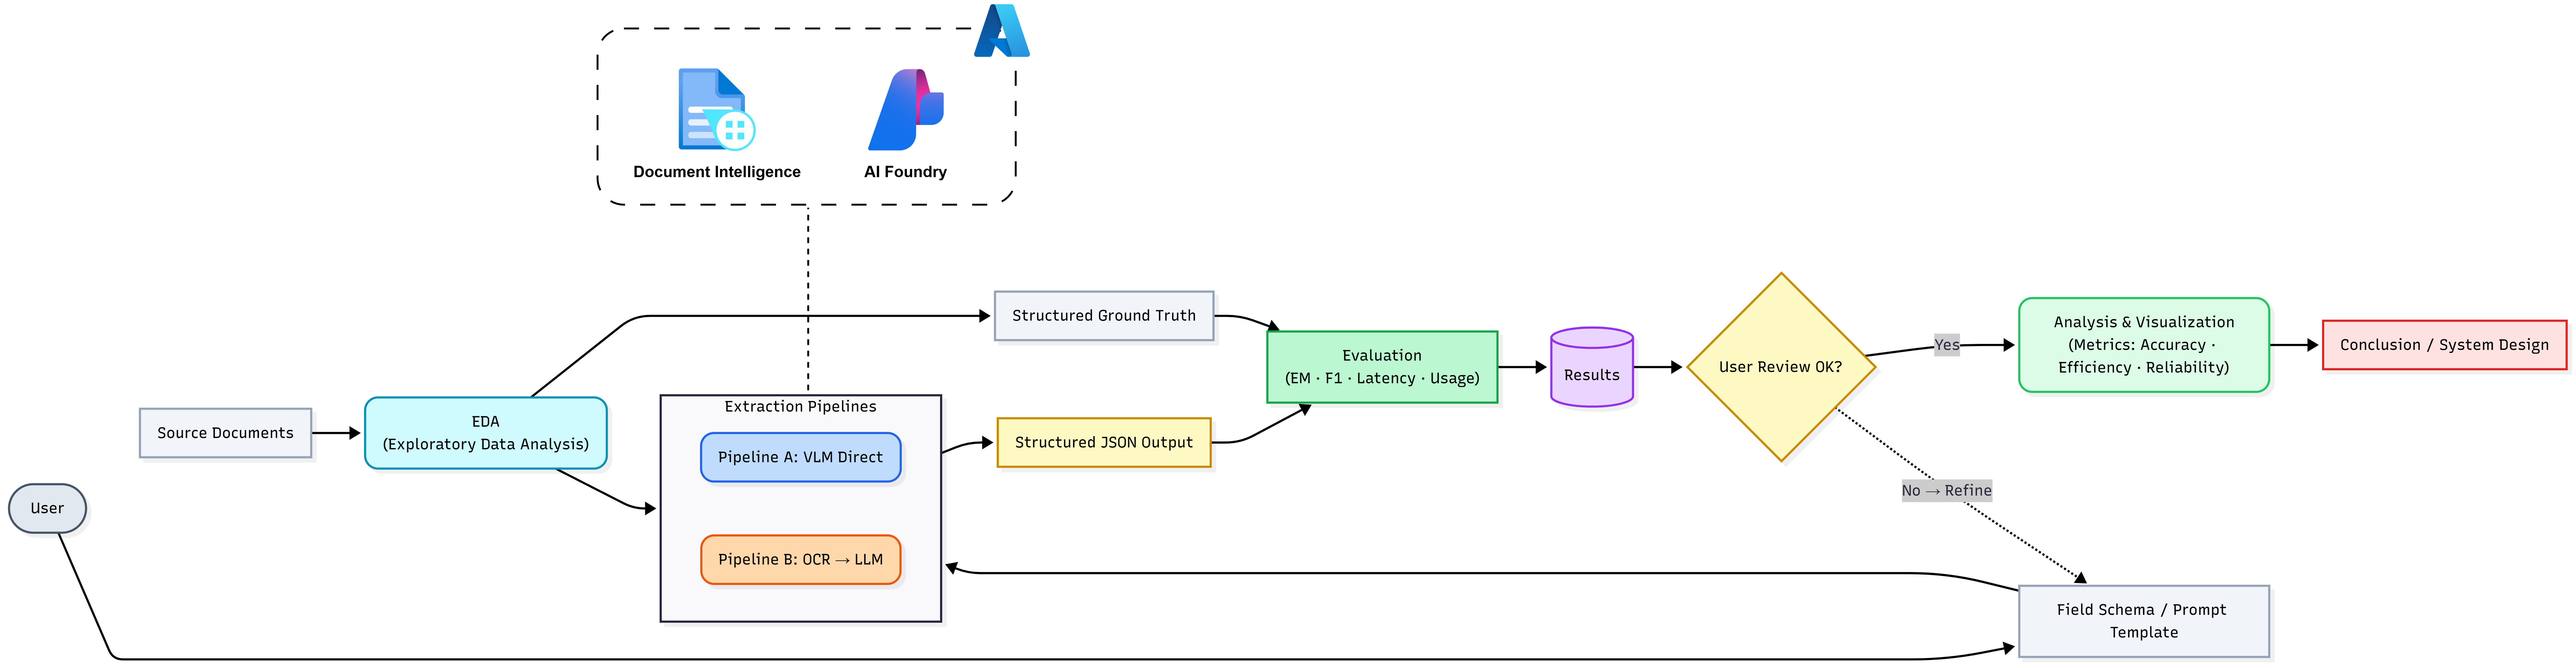
\includegraphics[width=0.9\linewidth]{Images/Overall-Workflow.png}
    \caption{Tổng quan kiến trúc hệ thống trích xuất dữ liệu có cấu trúc}
    \label{fig:overall_workflow}
\end{figure}

\begin{enumerate}
    \item \textbf{Chuẩn bị tài liệu nguồn (Source Documents):} Tập hợp tài liệu đầu vào gồm hóa đơn, căn cước công dân và hợp đồng, bao gồm cả tài liệu tiếng Anh lẫn tiếng Việt, dạng đánh máy và viết tay.

    \item \textbf{Phân tích khám phá dữ liệu (Exploratory Data Analysis - EDA):} Tác giả tiến hành khám phá dữ liệu để nắm đặc điểm phân bố, chất lượng ảnh, ngôn ngữ và cấu trúc của từng tập tài liệu. Từ bước này, quy trình tách thành hai nhánh song song: cấu hình pipeline và xây dựng ground truth từ tập dữ liệu.

    \item \textbf{Cấu hình Field Schema và Prompt Template:} Người dùng định nghĩa schema các trường cần trích xuất và prompt template cho từng loại tài liệu. Hai pipeline đọc cấu hình này để render prompt và lọc kết quả đầu ra.

    \item \textbf{Xây dựng ground truth có cấu trúc (Structured Ground Truth):} Từ kết quả EDA, tác giả xây dựng tập ground truth có cấu trúc, mỗi tài liệu được gắn nhãn thủ công theo đúng schema đã định nghĩa, phục vụ đánh giá.

    \item \textbf{Chạy hai pipeline song song:}
    \begin{itemize}
        \item \textbf{Pipeline A (VLM Direct):} Đưa ảnh tài liệu trực tiếp vào VLM cùng với prompt; mô hình trả về JSON mà không qua bước OCR. Các mô hình VLM được triển khai qua Azure AI Foundry.
        \item \textbf{Pipeline B (OCR-LLM):} Trích xuất văn bản từ ảnh qua OCR engine (EasyOCR hoặc Azure Document Intelligence), sau đó đưa văn bản vào LLM để parse JSON. LLM không nhận ảnh, chỉ nhận văn bản thuần.
    \end{itemize}

    \item \textbf{Kết quả JSON có cấu trúc (Structured JSON Output):} Cả hai pipeline đều tạo ra kết quả thống nhất dạng JSON có cấu trúc, theo đúng schema đã định nghĩa.

    \item \textbf{Đánh giá (Evaluation):} Mỗi tài liệu được đánh giá theo các chỉ số: EM, Token-F1, latency và lượng token tiêu thụ, được so sánh với ground truth.

    \item \textbf{Lưu kết quả (Results):} Kết quả đánh giá được lưu lại để người dùng kiểm tra.

    \item \textbf{Người dùng kiểm tra kết quả và phân nhánh:}
    \begin{itemize}
        \item Nếu kết quả đạt yêu cầu: chuyển sang bước Phân tích và Trực quan hóa, sau đó đưa ra Kết luận và Thiết kế hệ thống.
        \item Nếu chưa đạt: quay lại bước 3 để điều chỉnh Field Schema và Prompt Template, rồi chạy lại pipeline.
    \end{itemize}
\end{enumerate}

Hệ thống được thiết kế theo ba nguyên tắc chính:

\begin{itemize}
    \item \textbf{Tách biệt cấu hình và xử lý:} Field Schema và Prompt Template được định nghĩa độc lập với pipeline. Hai pipeline chỉ đọc và render cấu hình, không tự xây dựng prompt, cho phép thay đổi schema hoặc prompt mà không sửa code pipeline.

    \item \textbf{Chuẩn hóa đầu ra:} Cả hai pipeline đều tạo ra Structured JSON Output theo cùng schema, đảm bảo bộ đánh giá có thể áp dụng thống nhất trên toàn bộ kết quả.

    \item \textbf{Vòng lặp tinh chỉnh có kiểm soát:} Sau mỗi lần chạy, người dùng xem xét kết quả và quyết định tinh chỉnh cấu hình hay tiến hành phân tích, tránh chạy lại toàn bộ pipeline không cần thiết.
\end{itemize}

Ba nguyên tắc này đảm bảo hệ thống có thể mở rộng linh hoạt theo từng loại tài liệu, đồng thời tạo điều kiện so sánh công bằng giữa hai pipeline trong suốt quá trình thực nghiệm.

\section{Dữ liệu thực nghiệm}\label{sec:datasets}

Tập benchmark được tác giả xây dựng gồm \textbf{60 mẫu}, trải rộng hai ngôn ngữ (EN, VN),
ba loại tài liệu (invoice, contract, id\_card) và hai dạng văn bản (typed, handwritten).
Mỗi mẫu bao gồm một ảnh trang đầu của tài liệu gốc (PNG hoặc JPEG tùy nguồn) và một file JSON ground truth.
Giá trị các trường được giữ nguyên văn như trên tài liệu, không chuẩn hóa. Toàn bộ bộ dữ liệu
benchmark, kết quả thực nghiệm và hình ảnh minh họa được công bố công khai tại kho lưu trữ của
đề tài \cite{pham2026repo}.

Xét theo nguồn gốc, dữ liệu được tổng hợp từ hai nhóm chính: nhóm \textbf{dữ liệu công khai}
gồm ba bộ dữ liệu (SROIE, Kaggle, Roboflow) đóng góp 45 mẫu, và nhóm \textbf{dữ liệu tự thu thập}
từ tài liệu thực tế đóng góp 15 mẫu. Bảng~\ref{tab:datasets} tổng hợp số lượng mẫu theo từng nguồn.

\begin{table}[h]
\centering
\caption{Tổng hợp dữ liệu thực nghiệm theo nguồn}
\label{tab:datasets}
\begin{tabular}{|l|l|c|c|c|}
\hline
\textbf{Nhóm} & \textbf{Nguồn} & \textbf{Loại tài liệu (dạng)} & \textbf{Lang} & \textbf{Mẫu} \\ \hline
\multirow{3}{*}{Công khai}   & SROIE           & invoice (typed)             & EN & 7 \\ \cline{2-5}
                             & Kaggle rubabq66 & invoice + contract (typed)  & EN & 33 \\ \cline{2-5}
                             & Roboflow CCCD   & id\_card (typed)            & VN & 5 \\ \hline
\multirow{3}{*}{Tự thu thập} & CCCD thực tế    & id\_card (typed)            & VN & 5 \\ \cline{2-5}
                             & HĐ cho vay      & contract (typed)            & VN & 5 \\ \cline{2-5}
                             & HĐ mở tài khoản & contract (handwritten)      & VN & 5 \\ \hline
\multicolumn{4}{|r|}{\textbf{Tổng}} & \textbf{60} \\ \hline
\end{tabular}
\end{table}

Có thể nhận thấy rằng hợp đồng là loại tài liệu có độ phủ rộng nhất, xuất hiện ở cả hai ngôn ngữ
và cả hai dạng văn bản. Tập tự thu thập tập trung hoàn toàn vào tiếng Việt, bù đắp cho sự thiếu
hụt dữ liệu tiếng Việt trong các bộ dữ liệu công khai.

\subsection{Nguồn dữ liệu}\label{sec:data_sources}

\textbf{SROIE} (Scanned Receipts OCR and Information Extraction)\cite{huang2019sroie} là bộ
dữ liệu biên lai siêu thị quét, công bố tại ICDAR 2019. Tác giả lấy 7 mẫu từ tập test, ánh
xạ ground truth có sẵn sang schema bốn trường của loại tài liệu invoice:
\texttt{company}, \texttt{date}, \texttt{address}, \texttt{total}. Toàn bộ là văn bản đánh
máy tiếng Anh, được gộp vào tập con \texttt{EN/Typed-Invoice}.

Bộ dữ liệu \textbf{Kaggle invoice-receipt-contract-ocr}\footnote{Kaggle: \url{https://kaggle.com/datasets/rubabq66/invoice-receipt-contract-ocr}}
cung cấp ảnh kèm annotation OCR cho ba loại tài liệu tiếng Anh; tác giả sử dụng hai phần:
\begin{itemize}
    \item \textbf{Invoice + receipt (13 mẫu):} 7 invoice và 6 receipt, ánh xạ về cùng
    schema bốn trường (\texttt{company}, \texttt{date}, \texttt{address}, \texttt{total})
    với SROIE và gộp vào \texttt{EN/Typed-Invoice} (tổng 20 mẫu invoice).
    \item \textbf{Contract (20 mẫu):} hợp đồng tổng hợp (synthetic contracts), ánh xạ sang
    schema bảy trường contract: \texttt{party\_a}, \texttt{party\_b}, \texttt{effective\_date},
    \texttt{term}, \texttt{governing\_law}, \texttt{contract\_number}, \texttt{contract\_value}.
\end{itemize}
Tác giả chọn bộ dữ liệu này thay cho CUAD\cite{hendrycks2021cuad} vì CUAD chỉ cung cấp văn
bản thuần túy mà không kèm ảnh tài liệu, không phù hợp với Pipeline A (VLM trích xuất trực
tiếp từ ảnh).

Bộ dữ liệu \textbf{Roboflow CCCD}\footnote{Roboflow CCCD dataset: \url{https://universe.roboflow.com/diop/clone-dataset-type-od}}
chứa ảnh thẻ Căn cước công dân Việt Nam kèm annotation dạng object detection (bounding box
cho từng trường). Tác giả chọn 5 mẫu và ánh xạ sang schema văn bản gồm sáu trường:
\texttt{dob}, \texttt{expire\_date}, \texttt{name}, \texttt{nationality},
\texttt{origin\_place}, \texttt{id\_num}; thuộc tập con \texttt{VN/Typed-IdCard}.

\textbf{Dữ liệu tự thu thập:} Do hạn chế về dữ liệu tiếng Việt công khai cho loại hợp đồng và CCCD, tác giả tự thu thập
15 mẫu từ tài liệu thực tế. Tập này gồm ba nhóm:
\begin{itemize}
    \item \textbf{CCCD thực tế (5 mẫu, typed):} ảnh quét thẻ Căn cước công dân thực, dùng
    chung schema sáu trường với phần Roboflow; gộp vào tập con \texttt{VN/Typed-IdCard}
    (tổng 10 mẫu id\_card).
    \item \textbf{Hợp đồng cho vay (5 mẫu, typed):} hợp đồng cho vay ngân hàng đánh máy,
    thuộc tập con \texttt{VN/Typed-Contract}.
    \item \textbf{Hợp đồng mở tài khoản (5 mẫu, handwritten):} giấy đăng ký mở tài khoản có
    phần thông tin khách hàng điền tay, thuộc tập con \texttt{VN/Handwritten-Contract}.
    Đây là trường hợp tài liệu hỗn hợp typed-handwritten thường gặp trong nghiệp vụ ngân hàng.
\end{itemize}
Ba nhóm tự thu thập dùng chung schema tương ứng (id\_card hoặc contract) với các mẫu công khai.

\subsection{Tiền xử lý dữ liệu}\label{sec:preprocessing}

Các tài liệu từ nguồn tự thu thập có định dạng gốc là TIFF nhiều trang; tác giả chỉ lấy trang
đầu và chuyển sang PNG để đồng nhất với toàn bộ tập benchmark. Quy trình tiền xử lý được thực
hiện bằng hai thư viện:

\begin{itemize}
    \item \textbf{TIFF sang PNG (Pillow\footnote{Pillow: \url{https://pillow.readthedocs.io}}):} Chuyển ảnh TIFF nhiều trang sang PNG, chỉ lấy trang đầu. Áp dụng cho toàn bộ ảnh quét CCCD và hợp đồng ngân hàng.
    \item \textbf{PDF sang PNG (PyMuPDF\footnote{PyMuPDF: \url{https://pymupdf.readthedocs.io}}):} Render trang đầu của tài liệu PDF sang ảnh PNG. Áp dụng khi tài liệu nguồn ở định dạng PDF.
\end{itemize}

Ground truth được xây dựng thủ công theo schema định nghĩa cho từng loại tài liệu, với nguyên tắc: giá trị các trường được giữ nguyên văn như trên tài liệu (không chuẩn hóa định dạng ngày tháng hay đơn vị tiền tệ); trường không xuất hiện hoặc không áp dụng trong tài liệu cụ thể được đặt là \texttt{null}.

\subsection{Phân tích khám phá dữ liệu (EDA)}\label{sec:eda}

Tác giả thực hiện phân tích khám phá dữ liệu (Exploratory Data Analysis -- EDA) nhằm nắm rõ
đặc điểm phân bố của tập benchmark theo các chiều ngôn ngữ, loại tài liệu, dạng văn bản và
nguồn gốc dữ liệu. Hình~\ref{fig:eda_overview} tổng hợp phân bố của toàn bộ 60 mẫu theo năm
tập con. Về ngôn ngữ, tiếng Anh chiếm khoảng hai phần ba với 40 mẫu (66,7\%), tiếng Việt chiếm
một phần ba với 20 mẫu (33,3\%); sự chênh lệch này phản ánh thực tế nguồn dữ liệu công khai cho
tiếng Anh phong phú hơn, trong khi dữ liệu tiếng Việt phần lớn phải tự thu thập. Về dạng văn
bản, văn bản đánh máy chiếm tỉ lệ áp đảo với 55 mẫu (91,7\%); viết tay
chỉ có 5 mẫu (8,3\%), toàn bộ đến từ hợp đồng mở tài khoản tiếng Việt. Đây là hạn chế cần lưu
ý: số mẫu handwritten nhỏ nên kết quả đánh giá robustness trên dạng viết tay chỉ mang tính
tham khảo.

\begin{figure}[H]
    \centering
    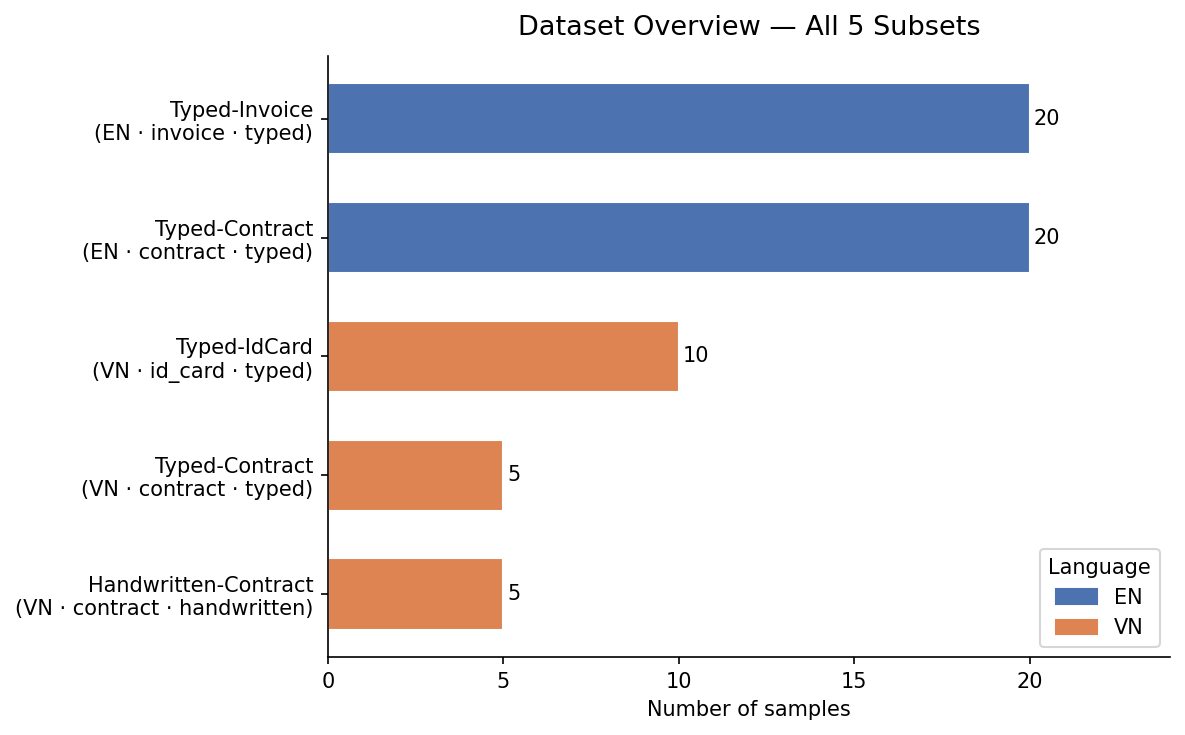
\includegraphics[width=\linewidth]{Images/fig7_dataset_overview.png}
    \caption{Tổng quan tập benchmark}
    \label{fig:eda_overview}
\end{figure}

Hình~\ref{fig:eda_lang_doctype} làm rõ sự giao thoa giữa ngôn ngữ và loại tài liệu: dữ liệu
tiếng Anh tập trung vào hóa đơn (20 mẫu) và hợp đồng (20 mẫu), trong khi tiếng Việt trải đều
giữa hợp đồng (10 mẫu) và CCCD (10 mẫu). Đáng chú ý, tiếng Việt không có mẫu hóa đơn và tiếng
Anh không có mẫu CCCD; sự lệch pha này là hệ quả trực tiếp của đặc thù nguồn dữ liệu và cần
được tính đến khi so sánh hiệu năng theo ngôn ngữ.

\begin{figure}[H]
    \centering
    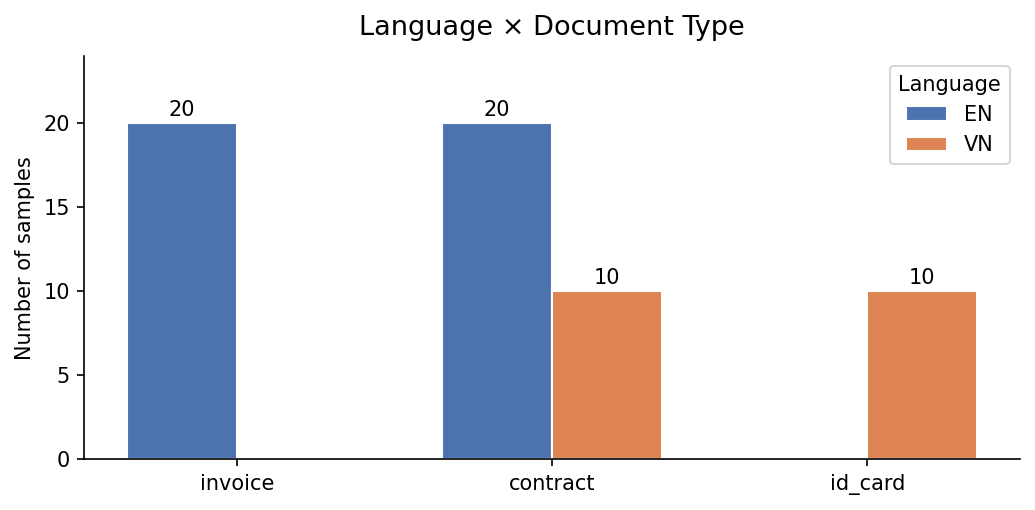
\includegraphics[width=0.85\linewidth]{Images/fig6_lang_x_doctype.png}
    \caption{Phân bố số mẫu theo ngôn ngữ và loại tài liệu}
    \label{fig:eda_lang_doctype}
\end{figure}

\section[Phương pháp và Pipeline trích xuất VLM Direct]{Phương pháp và Pipeline trích xuất VLM Direct (Pipeline A)}\label{sec:vlm_pipeline}

Pipeline A triển khai phương pháp VLM Direct Extraction, tức là không qua bước nhận dạng văn bản trung gian. Ảnh tài liệu được mã hóa thành biểu diễn số và truyền trực tiếp vào mô hình cùng với prompt, sau đó mô hình sinh ra đầu ra JSON có cấu trúc trong một lần gọi API duy nhất. Cách tiếp cận này loại bỏ sai số tích lũy từ khâu OCR và cho phép mô hình tận dụng cả thông tin thị giác lẫn ngữ nghĩa văn bản để suy luận về nội dung tài liệu. Hình~\ref{fig:pipeline_a} minh họa luồng xử lý tổng quát của Pipeline A.

\begin{figure}[H]
    \centering
    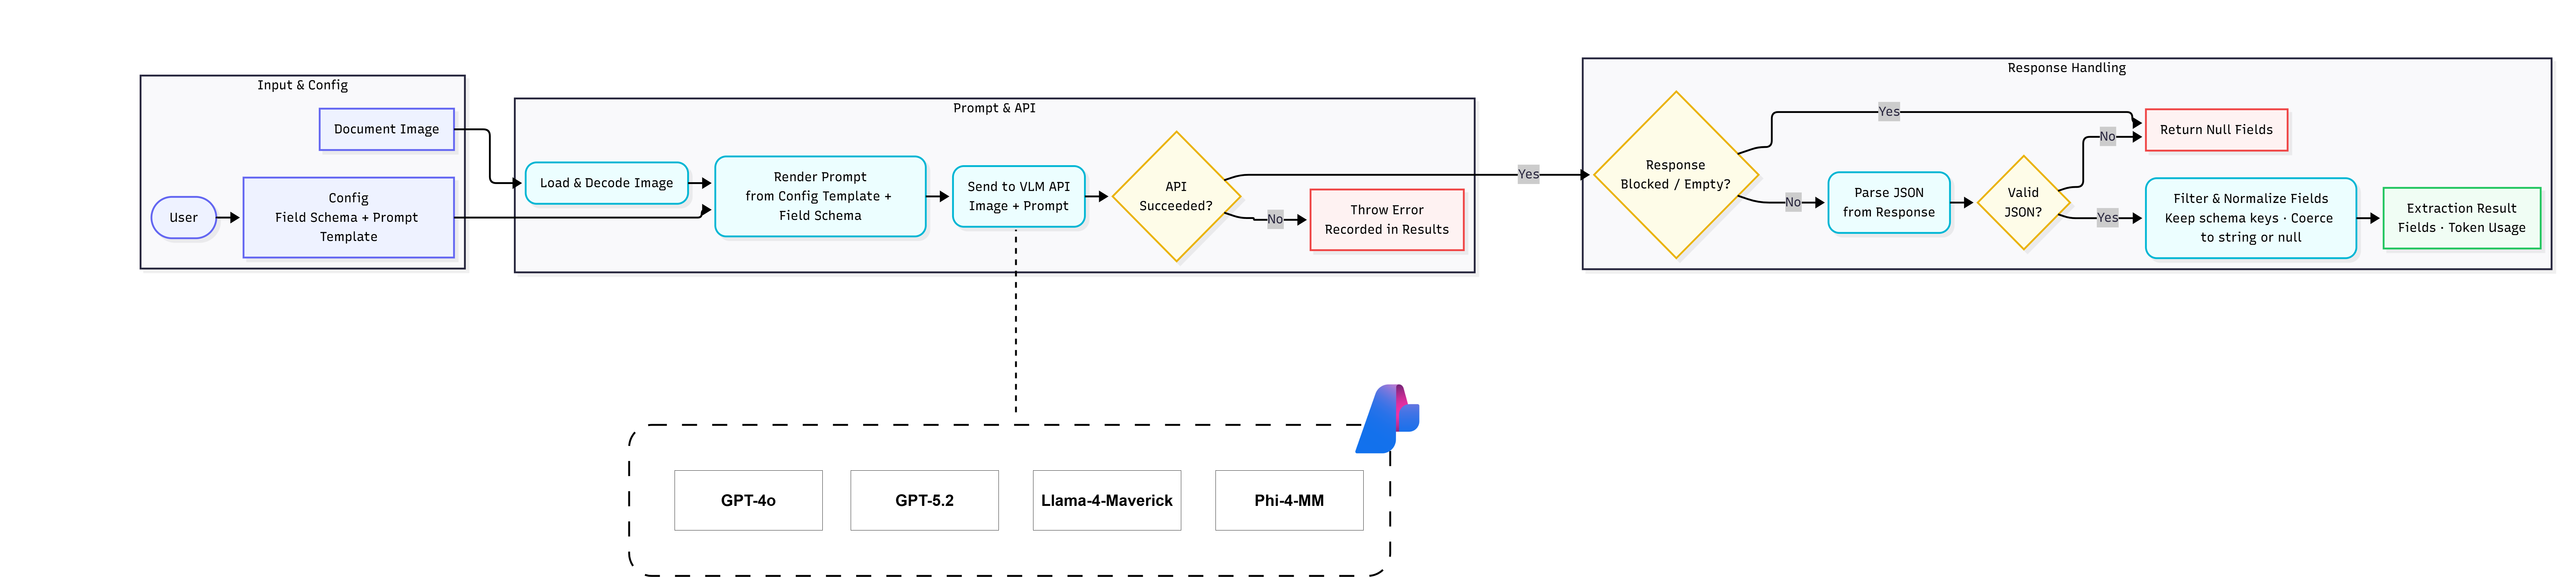
\includegraphics[width=\linewidth]{Images/Pipeline-VLM_Direct.png}
    \caption{Luồng xử lý của Pipeline A (VLM Direct Extraction)}
    \label{fig:pipeline_a}
\end{figure}

\subsection{Cấu hình Field Schema và Prompt Template}\label{sec:vlm_config}

Toàn bộ thông tin về trường cần trích xuất và hướng dẫn cho mô hình được tách biệt khỏi pipeline, lưu trong hai loại file cấu hình.

\textbf{Field Schema} (file cấu hình theo từng loại tài liệu) định nghĩa danh sách trường cần trích xuất cùng mô tả và định dạng kỳ vọng. Ví dụ, field schema cho loại tài liệu hóa đơn gồm bốn trường:

\begin{minted}{json}
{
  "company": { "description": "Tên công ty hoặc cửa hàng phát hành",
               "format": "giữ nguyên tên đầy đủ như in trên tài liệu" },
  "date":    { "description": "Ngày phát hành hóa đơn",
               "format": "giữ nguyên định dạng như in trên tài liệu" },
  "address": { "description": "Địa chỉ công ty",
               "format": "giữ nguyên như in; null nếu không có" },
  "total":   { "description": "Tổng số tiền phải thanh toán",
               "format": "giữ nguyên ký hiệu tiền tệ và định dạng số" }
}
\end{minted}

\textbf{Prompt Template} (file template prompt) chứa chỉ dẫn cho mô hình với các vị trí giữ chỗ dành cho field schema và danh sách tên trường. Tại thời điểm chạy, hệ thống điền các vị trí này từ field schema tương ứng, tạo ra prompt hoàn chỉnh. Nguyên tắc thiết kế prompt: yêu cầu mô hình trả về duy nhất JSON object, giữ nguyên giá trị như trên tài liệu (không chuẩn hóa ngày tháng, tiền tệ, chữ hoa/thường), và đặt \texttt{null} cho trường không tìm thấy.

Thiết kế tách biệt cấu hình khỏi pipeline cho phép thay đổi schema hoặc prompt cho từng loại tài liệu mà không cần sửa pipeline, đồng thời đảm bảo cả hai pipeline (A và B) dùng cùng một field config, tạo điều kiện so sánh công bằng.

\subsection{Thiết kế Pipeline A}\label{sec:vlm_design}

Pipeline A kế thừa từ lớp cơ sở chung và thực hiện quy trình trích xuất qua bốn bước chính:

\begin{enumerate}
    \item \textbf{Kiểm tra năng lực thị giác của mô hình}: Khi khởi tạo, pipeline kiểm tra xem mô hình được cấu hình có khả năng xử lý ảnh hay không. Nếu là mô hình ngôn ngữ thuần văn bản (như DeepSeek-V4), pipeline báo lỗi ngay khi khởi tạo để tránh gọi API với đầu vào không hợp lệ.

    \item \textbf{Tải ảnh và tạo prompt}: Ảnh tài liệu được tải vào bộ nhớ bằng Pillow\footnote{Pillow: \url{https://pillow.readthedocs.io}}, sau đó prompt hoàn chỉnh được tạo bằng cách điền field schema và danh sách tên trường vào template. Ảnh được giữ nguyên để lớp client chuyển đổi sang định dạng phù hợp với từng nhà cung cấp API ở bước tiếp theo.

    \item \textbf{Gọi VLM với cơ chế thử lại theo hàm mũ (exponential backoff)}: Mỗi lần gọi API đều có cơ chế thử lại tự động, tối đa 5 lần. Giữa các lần gọi, pipeline chủ động đợi một khoảng thời gian tối thiểu để tránh vượt giới hạn tốc độ của nhà cung cấp. Khi nhận phản hồi lỗi vượt giới hạn (HTTP 429), hệ thống ưu tiên đọc thời gian chờ đề xuất từ phía server thay vì tự tính toán.

    \item \textbf{Trích xuất JSON từ phản hồi}: Phản hồi thô từ mô hình được xử lý để loại bỏ các phần định dạng bao bọc (markdown fence nếu có), sau đó JSON object được trích xuất và parse. Kết quả được lọc để chỉ giữ các trường trong schema đã định nghĩa; giá trị được chuyển về kiểu chuỗi hoặc \texttt{null}. Nếu mô hình không trả về JSON hợp lệ (bị chặn bởi bộ lọc nội dung hoặc lỗi phân tích), pipeline ghi log cảnh báo và trả về tất cả trường là \texttt{null}.
\end{enumerate}

Mỗi lần trích xuất trả về một bộ kết quả thống nhất gồm: giá trị các trường đã trích xuất, thống kê số token tiêu thụ từ API, và metadata bổ sung. Định dạng đầu ra nhất quán giữa hai pipeline giúp module đánh giá áp dụng cùng một bộ chỉ số mà không cần xử lý riêng cho từng pipeline.

\subsection{Các mô hình thực nghiệm và nhà cung cấp}\label{sec:vlm_models}

Để phục vụ nhiều nhà cung cấp API khác nhau, tác giả thiết kế một giao diện thống nhất nhận vào prompt và ảnh (tùy chọn), trả về phản hồi và thống kê token. Mỗi nhà cung cấp được triển khai thành một lớp riêng:

\begin{itemize}
    \item \textbf{Azure OpenAI}\footnotemark: Gọi dịch vụ Azure OpenAI dành cho các mô hình GPT-4o và GPT-5. Ảnh được mã hóa thành chuỗi base64 trước khi gửi theo định dạng API yêu cầu. Lưu ý kỹ thuật: một số mô hình GPT-5 không chấp nhận tham số nhiệt độ trong yêu cầu, nên pipeline tự động bỏ qua tham số này khi cần thiết.
    \footnotetext{OpenAI Python SDK: \url{https://github.com/openai/openai-python}}

    \item \textbf{Azure AI Foundry}\footnotemark: Gọi nền tảng Azure AI Foundry cho các mô hình Phi-4-multimodal-instruct, Llama-4-Maverick và DeepSeek-V4-Flash. Ảnh được mã hóa theo cùng định dạng base64. Với DeepSeek-V4-Flash là mô hình thuần văn bản, Pipeline A tự động từ chối sử dụng nó và chỉ được phép dùng trong Pipeline B.
    \footnotetext{Azure AI Inference SDK: \url{https://pypi.org/project/azure-ai-inference/}}
\end{itemize}

Thiết kế này đảm bảo pipeline không phụ thuộc vào bất kỳ SDK cụ thể nào; thay đổi nhà cung cấp chỉ cần cập nhật cấu hình môi trường mà không ảnh hưởng đến logic xử lý của cả hai pipeline.

\begin{table}[h]
\centering
\caption{Danh sách mô hình VLM sử dụng trong Pipeline A}
\label{tab:models_pipeline_a}
\begin{tabular}{|l|l|l|}
\hline
\textbf{Mô hình} & \textbf{Model ID} & \textbf{Nhà cung cấp} \\ \hline
GPT-5.2          & \texttt{gpt-5.2-chat}                             & Azure OpenAI  \\ \hline
GPT-4o           & \texttt{gpt-4o}                                   & Azure OpenAI  \\ \hline
Llama-4-Maverick & \texttt{Llama-4-Maverick-17B-128E-Instruct-FP8}   & Azure Foundry \\ \hline
Phi-4-MM         & \texttt{Phi-4-multimodal-instruct}                & Azure Foundry \\ \hline
\end{tabular}
\end{table}

\paragraph{Nhận xét:}
Pipeline A có ưu điểm về độ trễ thấp nhờ loại bỏ bước OCR trung gian và giảm số lần gọi API xuống còn một. Tuy nhiên, yêu cầu bắt buộc mô hình phải có khả năng thị giác hạn chế số lựa chọn mô hình, và chất lượng trích xuất phụ thuộc trực tiếp vào năng lực nhận dạng chữ viết của VLM, đặc biệt với văn bản tiếng Việt và chữ viết tay.

% -----------------------------------------------------------------------

\section[Phương pháp và Pipeline trích xuất OCR-LLM]{Phương pháp và Pipeline trích xuất OCR-LLM (Pipeline B)}\label{sec:ocr_llm_pipeline}

Pipeline B chia bài toán trích xuất thành hai giai đoạn tách biệt: giai đoạn OCR và giai đoạn phân tích cú pháp ngữ nghĩa bằng LLM. Ảnh tài liệu trước tiên được đưa qua engine OCR để trích xuất văn bản thuần dạng chuỗi, sau đó chuỗi văn bản đó được đưa vào LLM cùng prompt để sinh ra JSON có cấu trúc. LLM ở bước hai không nhận ảnh, chỉ xử lý văn bản. Phương pháp này cho phép sử dụng các OCR engine chuyên biệt được tối ưu cho từng ngôn ngữ, cũng như mô hình ngôn ngữ thuần văn bản không có khả năng thị giác. Hình~\ref{fig:pipeline_b} minh họa luồng xử lý tổng quát của Pipeline B.

\begin{figure}[H]
    \centering
    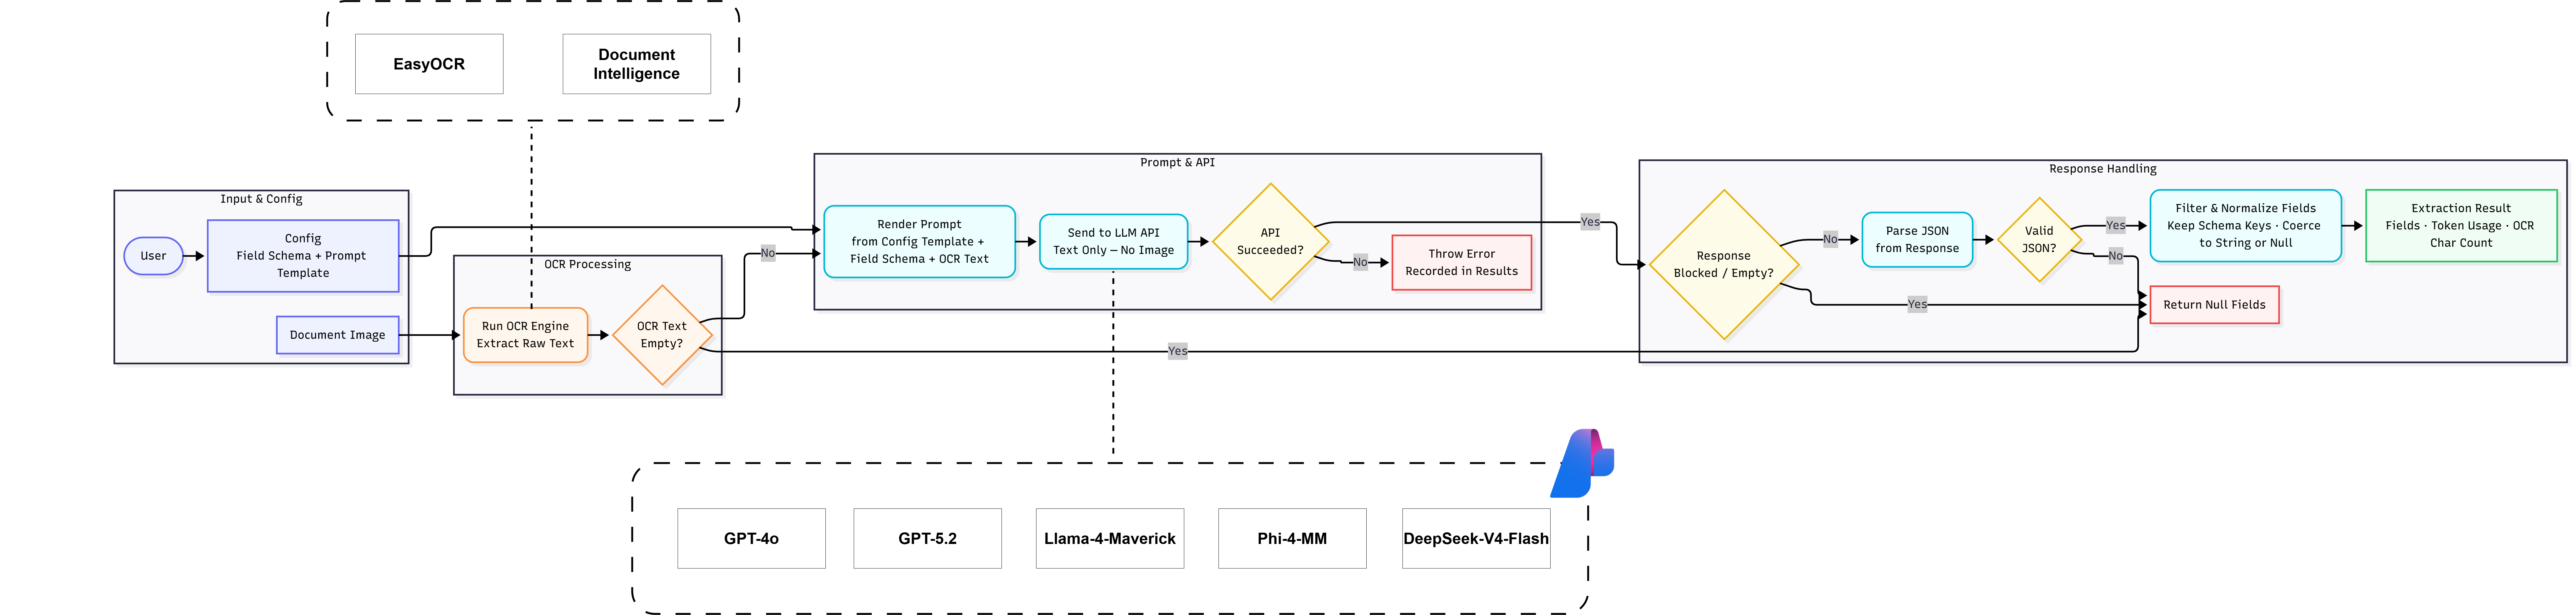
\includegraphics[width=\linewidth]{Images/Pipeline-OCR-LLM.png}
    \caption{Luồng xử lý của Pipeline B (OCR-LLM)}
    \label{fig:pipeline_b}
\end{figure}

\subsection{Giai đoạn OCR: các engine nhận dạng văn bản}\label{sec:ocr_engines}

Tác giả thiết kế cơ chế cho phép thay thế engine OCR mà không ảnh hưởng đến phần còn lại của pipeline. Hai engine được sử dụng trong thực nghiệm:

\begin{itemize}
    \item \textbf{EasyOCR}\footnotemark: thư viện OCR mã nguồn mở chạy cục bộ, hỗ trợ hơn 80 ngôn ngữ bao gồm tiếng Anh và tiếng Việt. Mô hình được tải về lần đầu và lưu vào bộ nhớ đệm cục bộ theo cơ chế khởi tạo trễ (lazy initialization), tránh chi phí khởi động không cần thiết khi engine chưa được gọi. EasyOCR nhận danh sách ngôn ngữ cần nhận dạng và trả về các đoạn văn bản theo từng vùng phát hiện được, sau đó được nối thành một chuỗi liên tục. Engine này phù hợp với môi trường không có kết nối cloud và không phát sinh chi phí API.
    \footnotetext{EasyOCR: \url{https://github.com/JaidedAI/EasyOCR}}

    \item \textbf{Azure Document Intelligence}\footnotemark: dịch vụ OCR đám mây của Microsoft Azure sử dụng model phân tích tài liệu đa ngôn ngữ có sẵn, trả về nội dung tài liệu theo thứ tự đọc tự nhiên. Engine cũng áp dụng khởi tạo trễ; thông tin xác thực (endpoint và API key) được đọc từ biến môi trường. Azure Document Intelligence có chất lượng OCR cao hơn cho tài liệu phức tạp, nhưng phát sinh chi phí theo số trang xử lý.
    \footnotetext{Azure AI Document Intelligence SDK: \url{https://pypi.org/project/azure-ai-documentintelligence/}}
\end{itemize}

Trong thực nghiệm chính, tác giả sử dụng EasyOCR cho các tập con tiếng Anh và Azure Document Intelligence cho các tập con tiếng Việt, phù hợp với yêu cầu nhận dạng chữ Việt có dấu thanh điệu.

\subsection{Giai đoạn LLM: phân tích cú pháp từ văn bản OCR}\label{sec:llm_parsing}

Prompt template cho Pipeline B khác với Pipeline A ở chỗ có thêm vị trí giữ chỗ dành cho văn bản OCR. Prompt cũng lưu ý rằng văn bản có thể chứa lỗi OCR hoặc các dòng không theo thứ tự, yêu cầu mô hình suy luận dựa trên ngữ cảnh để trích xuất giá trị chính xác nhất. Các yêu cầu còn lại giống Pipeline A: chỉ trả về JSON object, giữ nguyên giá trị như trên tài liệu, \texttt{null} cho trường không xác định được.

Pipeline B sử dụng cùng cơ chế gọi API như Pipeline A, nhưng không yêu cầu mô hình phải hỗ trợ thị giác. Do đó, ngoài bốn mô hình VLM đã liệt kê ở \hyperref[sec:vlm_models]{Mục 4.3.3}, Pipeline B còn chạy thêm DeepSeek-V4-Flash, mô hình ngôn ngữ thuần văn bản triển khai qua Azure AI Foundry.

\begin{table}[h]
\centering
\caption{Danh sách mô hình sử dụng trong Pipeline B (bao gồm cả mô hình thuần văn bản)}
\label{tab:models_pipeline_b}
\begin{tabular}{|l|l|l|}
\hline
\textbf{Mô hình} & \textbf{Model ID} & \textbf{Nhà cung cấp} \\ \hline
GPT-5.2          & \texttt{gpt-5.2-chat}                             & Azure OpenAI  \\ \hline
GPT-4o           & \texttt{gpt-4o}                                   & Azure OpenAI  \\ \hline
Llama-4-Maverick & \texttt{Llama-4-Maverick-17B-128E-Instruct-FP8}   & Azure Foundry \\ \hline
Phi-4-MM         & \texttt{Phi-4-multimodal-instruct}                & Azure Foundry \\ \hline
DeepSeek-V4      & \texttt{DeepSeek-V4-Flash}                        & Azure Foundry \\ \hline
\end{tabular}
\end{table}

\subsection{Thiết kế Pipeline B}\label{sec:ocr_llm_design}

Pipeline B kế thừa từ lớp cơ sở chung và thực hiện quy trình năm bước:

\begin{enumerate}
    \item \textbf{Chạy OCR}: Ảnh được đưa qua engine OCR đã cấu hình (mặc định là EasyOCR). Nếu engine không trả về văn bản nào (ảnh quá nhiễu hoặc không có chữ viết), pipeline dừng sớm và ghi log cảnh báo mà không tiêu tốn token LLM.

    \item \textbf{Ghi nhận thông tin chất lượng OCR}: Số ký tự trong chuỗi văn bản trích xuất được lưu vào metadata của kết quả, phục vụ phân tích lỗi sau thực nghiệm. Thông tin này giúp phân biệt trường hợp mô hình thất bại do chất lượng OCR thấp với trường hợp thất bại do mô hình suy luận sai.

    \item \textbf{Tạo prompt với văn bản OCR}: Văn bản OCR được chèn vào template prompt cùng với field schema và danh sách tên trường, tạo thành prompt hoàn chỉnh dạng văn bản thuần cho LLM.

    \item \textbf{Gọi LLM với cơ chế thử lại}: Lần gọi này mô hình chỉ nhận văn bản, không có ảnh. Cơ chế thử lại và điều tiết tốc độ giống Pipeline A, được kế thừa từ lớp cơ sở chung.

    \item \textbf{Trích xuất JSON từ phản hồi}: Phản hồi được xử lý theo cách tương tự Pipeline A: loại bỏ phần định dạng bao bọc, trích xuất JSON, lọc trường và chuẩn hóa kiểu dữ liệu.
\end{enumerate}

Việc tách OCR và LLM thành hai giai đoạn độc lập mang lại khả năng kiểm tra từng thành phần riêng biệt: khi kết quả không chính xác, thông tin số ký tự OCR trong metadata giúp xác định liệu lỗi xuất phát từ khâu nhận dạng văn bản hay từ khâu suy luận của mô hình.

\paragraph{Nhận xét:}
Phương pháp OCR-LLM có ưu điểm về tính linh hoạt: engine OCR có thể thay thế cho phép chọn công cụ chuyên biệt phù hợp với từng ngôn ngữ hoặc loại tài liệu, và pipeline hoạt động được với cả mô hình ngôn ngữ thuần văn bản. Tuy nhiên, việc chia thành hai bước làm tăng độ trễ tổng thể và đưa vào một nguồn lỗi bổ sung từ khâu OCR, đặc biệt rõ rệt trên tài liệu chữ viết tay hoặc ảnh chất lượng thấp.

\section{Kết quả thực nghiệm}\label{sec:results}

Trong mục này, tác giả trình bày kết quả đánh giá định lượng của hai chiến lược trích xuất trên bộ dữ liệu thực nghiệm, lần lượt theo bốn chiều: độ chính xác, độ bền vững, hiệu quả và độ tin cậy.

\subsection{Điều kiện thực nghiệm}\label{sec:experiment_setup}

Tác giả đánh giá năm mô hình trên hai chiến lược trích xuất là VLM Direct và OCR-LLM, với tổng cộng 540 lượt trích xuất tài liệu. Mô hình DeepSeek-V4 là mô hình ngôn ngữ thuần văn bản nên chỉ chạy ở pipeline OCR-LLM, trong khi bốn mô hình còn lại được chạy ở cả hai pipeline. Nhằm bảo đảm tính tái lập và so sánh công bằng, toàn bộ thực nghiệm được chuẩn hóa theo các điều kiện sau:

\begin{itemize}
    \item \textbf{Prompt}: Dùng cùng một prompt cho mọi mô hình trong cùng pipeline.
    \item \textbf{Schema}: Yêu cầu cùng một schema JSON phẳng cho từng loại tài liệu.
    \item \textbf{Độ phân giải}: Đưa ảnh đầu vào ở cùng độ phân giải.
    \item \textbf{Tham số sinh}: Đặt \texttt{temperature=0} để loại bỏ tính ngẫu nhiên.
\end{itemize}

Việc đánh giá được tiến hành theo bốn chiều, mỗi chiều phản ánh một khía cạnh khác nhau của chất lượng trích xuất:

\begin{itemize}
    \item \textbf{Độ chính xác (Accuracy)}: Đo bằng EM và Token-F1.
    \item \textbf{Độ bền vững (Robustness)}: Mức sụt giảm độ chính xác khi chuyển từ văn bản đánh máy sang viết tay và từ tiếng Anh sang tiếng Việt.
    \item \textbf{Hiệu quả (Efficiency)}: Độ trễ tính bằng giây trên mỗi tài liệu và chi phí tính bằng USD trên 1000 tài liệu.
    \item \textbf{Độ tin cậy (Reliability)}: Tỉ lệ hallucination và tỉ lệ tuân thủ schema.
\end{itemize}

Chi phí trong các phân tích dưới đây được ước tính theo đơn giá token niêm yết công khai của từng nhà cung cấp tại thời điểm tháng 5/2026 (Bảng~\ref{tab:pricing}). Với mỗi tài liệu, chi phí được tính bằng công thức $(t_{in}\,p_{in} + t_{out}\,p_{out})/10^{6}$, trong đó $t_{in}$ và $t_{out}$ lần lượt là số token đầu vào và đầu ra, $p_{in}$ và $p_{out}$ là đơn giá tương ứng trên một triệu token; kết quả được quy đổi sang USD trên 1000 tài liệu để tiện so sánh. Đơn giá được tổng hợp từ trang giá chính thức của Azure OpenAI và Azure AI Foundry\footnote{Azure OpenAI pricing: \url{https://azure.microsoft.com/pricing/details/azure-openai/}; Azure AI Foundry models pricing: \url{https://azure.microsoft.com/pricing/details/ai-foundry-models/}} cho các mô hình GPT, Llama và Phi, cùng trang giá API của DeepSeek\footnote{DeepSeek API pricing: \url{https://api-docs.deepseek.com/quick_start/pricing}} cho DeepSeek-V4-Flash (truy cập tháng 5/2026).

\begin{table}[h]
\centering
\caption{Đơn giá token của các mô hình thực nghiệm (USD trên một triệu token, tổng hợp tháng 5/2026)}
\label{tab:pricing}
\begin{tabular}{|l|c|c|c|}
\hline
\textbf{Mô hình} & \textbf{Đầu vào (\$/1M)} & \textbf{Đầu ra (\$/1M)} & \textbf{Thị giác} \\ \hline
GPT-5.2           & 1,75       & 14,00 & $\checkmark$ \\ \hline
GPT-4o            & 2,50       & 10,00 & $\checkmark$ \\ \hline
Llama-4-Maverick  & 0,35$^{*}$ & 0,60  & $\checkmark$ \\ \hline
Phi-4-MM          & 0,08       & 0,32  & $\checkmark$ \\ \hline
DeepSeek-V4-Flash & 0,14       & 0,28  & $\times$ \\ \hline
\end{tabular}

\vspace{2pt}
{\footnotesize $^{*}$Azure niêm yết Llama-4-Maverick theo khoảng 0,15--0,50 \$/1M token đầu vào; tác giả lấy giá trị đại diện 0,35 để ước tính. Cột Thị giác cho biết mô hình có khả năng xử lý ảnh hay không: DeepSeek-V4-Flash là mô hình thuần văn bản nên chỉ chạy ở Pipeline B.}
\end{table}

Bảng~\ref{tab:leaderboard} tổng hợp kết quả của từng cặp mô hình và pipeline, sắp xếp theo EM giảm dần.

\begin{table}[h]
\centering
\caption{Bảng tổng hợp kết quả thực nghiệm theo bốn chiều đánh giá}
\label{tab:leaderboard}
\footnotesize
\renewcommand{\arraystretch}{1.3}
\begin{tabular}{|p{3cm}|p{1.7cm}|c|c|c|c|c|c|}
\hline
\textbf{Mô hình} & \textbf{Pipeline} & \textbf{EM} & \textbf{F1} & \textbf{Độ trễ (s)} & \textbf{Chi phí (USD/1k)} & \textbf{Hallu.} & \textbf{Schema} \\ \hline
Llama-4-Maverick & VLM Direct & \cellcolor{yellow!25}\textbf{83,6\%} & \cellcolor{yellow!25}\textbf{92,3\%} & \cellcolor{yellow!25}\textbf{1,76} & 0,91 & 2,6\% & 100\% \\ \hline
GPT-4o & VLM Direct & 82,4\% & 89,9\% & 3,95 & 3,63 & 6,3\% & 100\% \\ \hline
GPT-5.2 & VLM Direct & 80,8\% & 92,1\% & 8,41 & 6,66 & \cellcolor{yellow!25}\textbf{0,0\%} & 100\% \\ \hline
DeepSeek-V4 & OCR-LLM & 78,6\% & 89,6\% & 10,70 & 0,13 & 0,5\% & 100\% \\ \hline
GPT-4o & OCR-LLM & 77,0\% & 86,6\% & 7,93 & 2,45 & 2,6\% & 100\% \\ \hline
Llama-4-Maverick & OCR-LLM & 76,9\% & 88,1\% & 9,86 & 0,28 & 3,0\% & 100\% \\ \hline
Phi-4-MM & VLM Direct & 72,3\% & 78,1\% & 12,55 & 0,30 & 26,8\% & 100\% \\ \hline
GPT-5.2 & OCR-LLM & 72,1\% & 88,2\% & 11,09 & 5,24 & \cellcolor{yellow!25}\textbf{0,0\%} & 100\% \\ \hline
Phi-4-MM & OCR-LLM & 70,2\% & 82,9\% & 11,80 & \cellcolor{yellow!25}\textbf{0,08} & 3,9\% & 98,3\% \\ \hline
\end{tabular}
\end{table}

\subsection{Kết quả độ chính xác tổng thể}\label{sec:results_doctype}

Kết quả thực nghiệm cho thấy ở phần lớn các mô hình, chiến lược VLM Direct đạt độ chính xác cao hơn OCR-LLM trên cả hai thước đo EM và Token-F1, như minh họa ở Hình~\ref{fig:accuracy_em} và Hình~\ref{fig:accuracy_f1}. Mô hình Llama-4-Maverick (VLM Direct) đạt kết quả cao nhất với EM bằng 83,6\% và Token-F1 bằng 92,3\%, trong khi DeepSeek-V4 dẫn đầu nhóm OCR-LLM với EM bằng 78,6\%, cho thấy một mô hình ngôn ngữ thuần văn bản vẫn có thể cạnh tranh khi được cung cấp văn bản OCR chất lượng tốt. Có thể nhận thấy rằng độ chênh lệch giữa EM và Token-F1 ở mọi mô hình là đáng kể, phản ánh hiện tượng kết quả trích xuất đúng về mặt ngữ nghĩa nhưng khác biệt ở mức ký tự.

\begin{figure}[H]
    \centering
    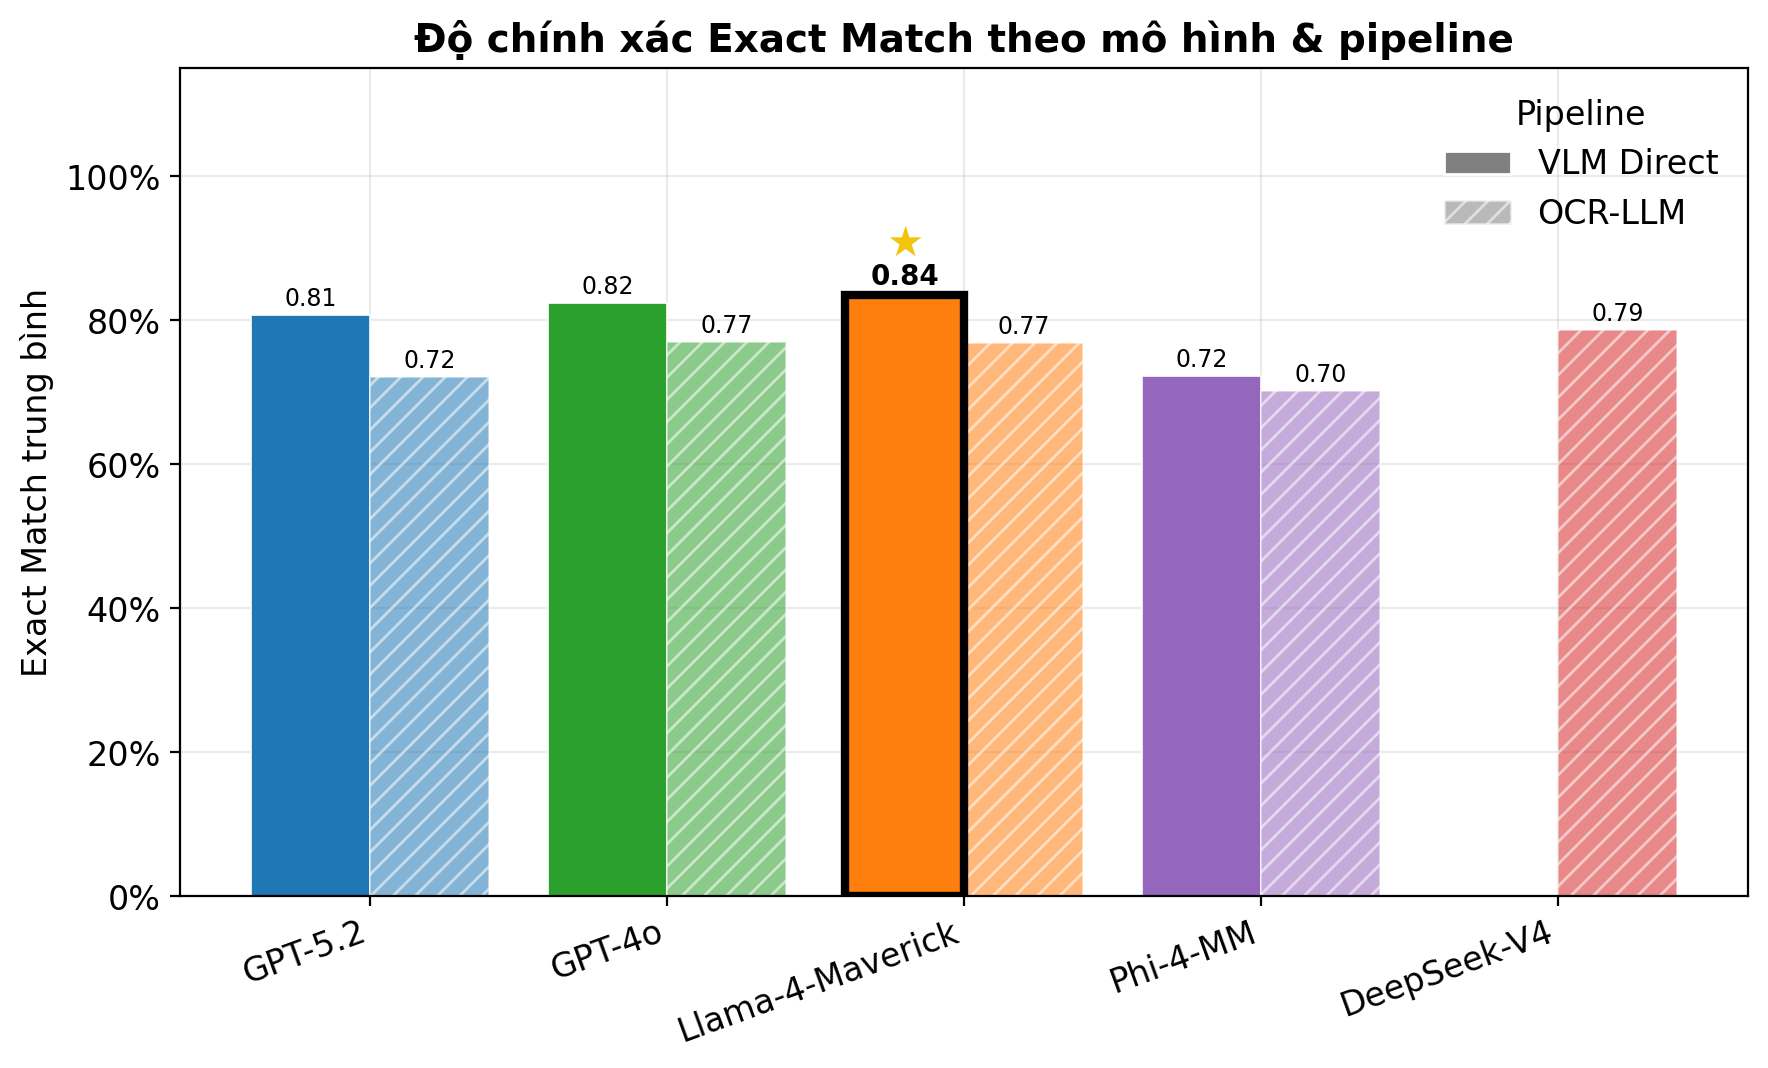
\includegraphics[width=0.8\linewidth]{Images/fig_accuracy_em.png}
    \caption{Độ chính xác Exact Match theo mô hình và pipeline}
    \label{fig:accuracy_em}
\end{figure}

\begin{figure}[H]
    \centering
    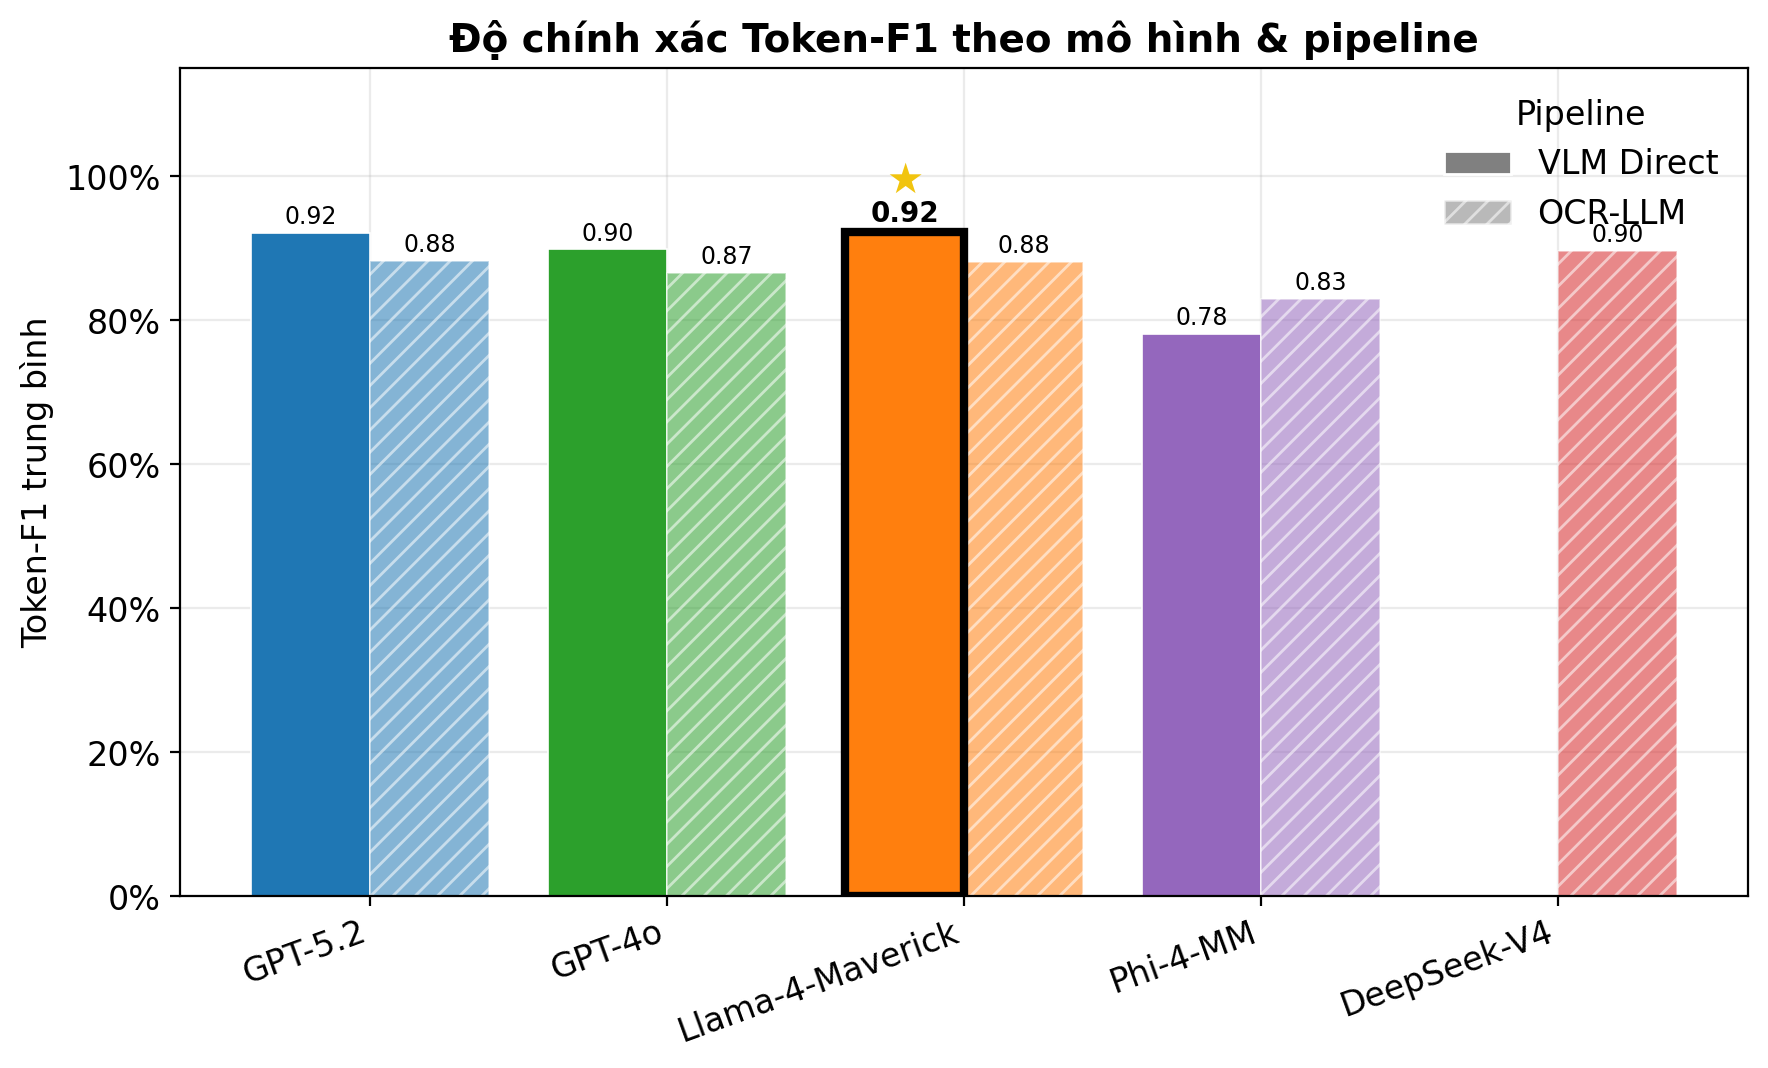
\includegraphics[width=0.8\linewidth]{Images/fig_accuracy_f1.png}
    \caption{Độ chính xác Token-F1 theo mô hình và pipeline}
    \label{fig:accuracy_f1}
\end{figure}

\subsection{Kết quả theo ngôn ngữ}\label{sec:results_lang}

Do đặc thù nguồn dữ liệu, tài liệu tiếng Anh và tiếng Việt khác nhau cả về loại văn bản lẫn độ khó, nên việc tách kết quả theo ngôn ngữ giúp đánh giá khả năng đa ngôn ngữ của từng mô hình. Bảng~\ref{tab:accuracy_lang} trình bày độ chính xác EM và Token-F1 tách riêng theo tiếng Anh và tiếng Việt cho từng cặp mô hình và pipeline. Các giá trị này là cơ sở để phân tích mức sụt giảm độ chính xác giữa hai ngôn ngữ ở phần thảo luận tiếp theo.

\begin{table}[h]
\centering
\caption{Độ chính xác EM / Token-F1 theo ngôn ngữ}
\label{tab:accuracy_lang}
\footnotesize
\renewcommand{\arraystretch}{1.3}
\begin{tabular}{|l|l|cc|cc|cc|}
\hline
\multirow{2}{*}{\textbf{Pipeline}} & \multirow{2}{*}{\textbf{Mô hình}} & \multicolumn{2}{c|}{\textbf{Tiếng Anh}} & \multicolumn{2}{c|}{\textbf{Tiếng Việt}} & \multicolumn{2}{c|}{\textbf{Tổng hợp}} \\ \cline{3-8}
 &  & \textbf{EM} & \textbf{F1} & \textbf{EM} & \textbf{F1} & \textbf{EM} & \textbf{F1} \\ \hline
\multirow{4}{*}{VLM Direct} & GPT-5.2          & 80,1\% & 92,5\% & 82,1\% & 91,5\% & 80,8\% & 92,1\% \\ \cline{2-8}
 & GPT-4o                                       & 86,0\% & 92,5\% & 75,4\% & 84,5\% & 82,4\% & 89,9\% \\ \cline{2-8}
 & Llama-4-Maverick                             & 82,5\% & 91,6\% & \cellcolor{yellow!25}\textbf{85,7\%} & \cellcolor{yellow!25}\textbf{93,7\%} & \cellcolor{yellow!25}\textbf{83,6\%} & \cellcolor{yellow!25}\textbf{92,3\%} \\ \cline{2-8}
 & Phi-4-MM                                     & \cellcolor{yellow!25}\textbf{88,8\%} & \cellcolor{yellow!25}\textbf{93,9\%} & 39,4\% & 46,4\% & 72,3\% & 78,1\% \\ \hline
\multirow{5}{*}{OCR-LLM}    & GPT-5.2          & 70,8\% & 86,5\% & 74,8\% & 91,6\% & 72,1\% & 88,2\% \\ \cline{2-8}
 & GPT-4o                                       & 78,8\% & 86,3\% & 73,5\% & 87,0\% & 77,0\% & 86,6\% \\ \cline{2-8}
 & Llama-4-Maverick                             & 77,6\% & 89,1\% & 75,5\% & 86,0\% & 76,9\% & 88,1\% \\ \cline{2-8}
 & Phi-4-MM                                     & 70,9\% & 82,8\% & 68,9\% & 83,1\% & 70,2\% & 82,9\% \\ \cline{2-8}
 & DeepSeek-V4                                  & 77,0\% & 87,5\% & 82,0\% & \cellcolor{yellow!25}\textbf{93,7\%} & 78,6\% & 89,6\% \\ \hline
\end{tabular}
\end{table}

Bản đồ nhiệt ở Hình~\ref{fig:robustness_heatmap} cho thấy sự phân hóa rõ rệt giữa các mô hình khi chuyển ngôn ngữ. Mô hình Phi-4-MM (VLM Direct) đạt EM tuyệt đối trên hợp đồng tiếng Anh đánh máy nhưng sụt giảm xuống còn 0,39--0,42 trên các tài liệu tiếng Việt, tương ứng mức giảm khoảng 0,49 điểm EM giữa hai ngôn ngữ. Ngược lại, DeepSeek-V4 (OCR-LLM) thể hiện độ bền vững tốt nhất khi điểm EM trên tiếng Việt (82,0\%) thậm chí cao hơn tiếng Anh (77,0\%), cho thấy ưu thế của khâu OCR chuyên biệt đối với tài liệu tiếng Việt.

\begin{figure}[H]
    \centering
    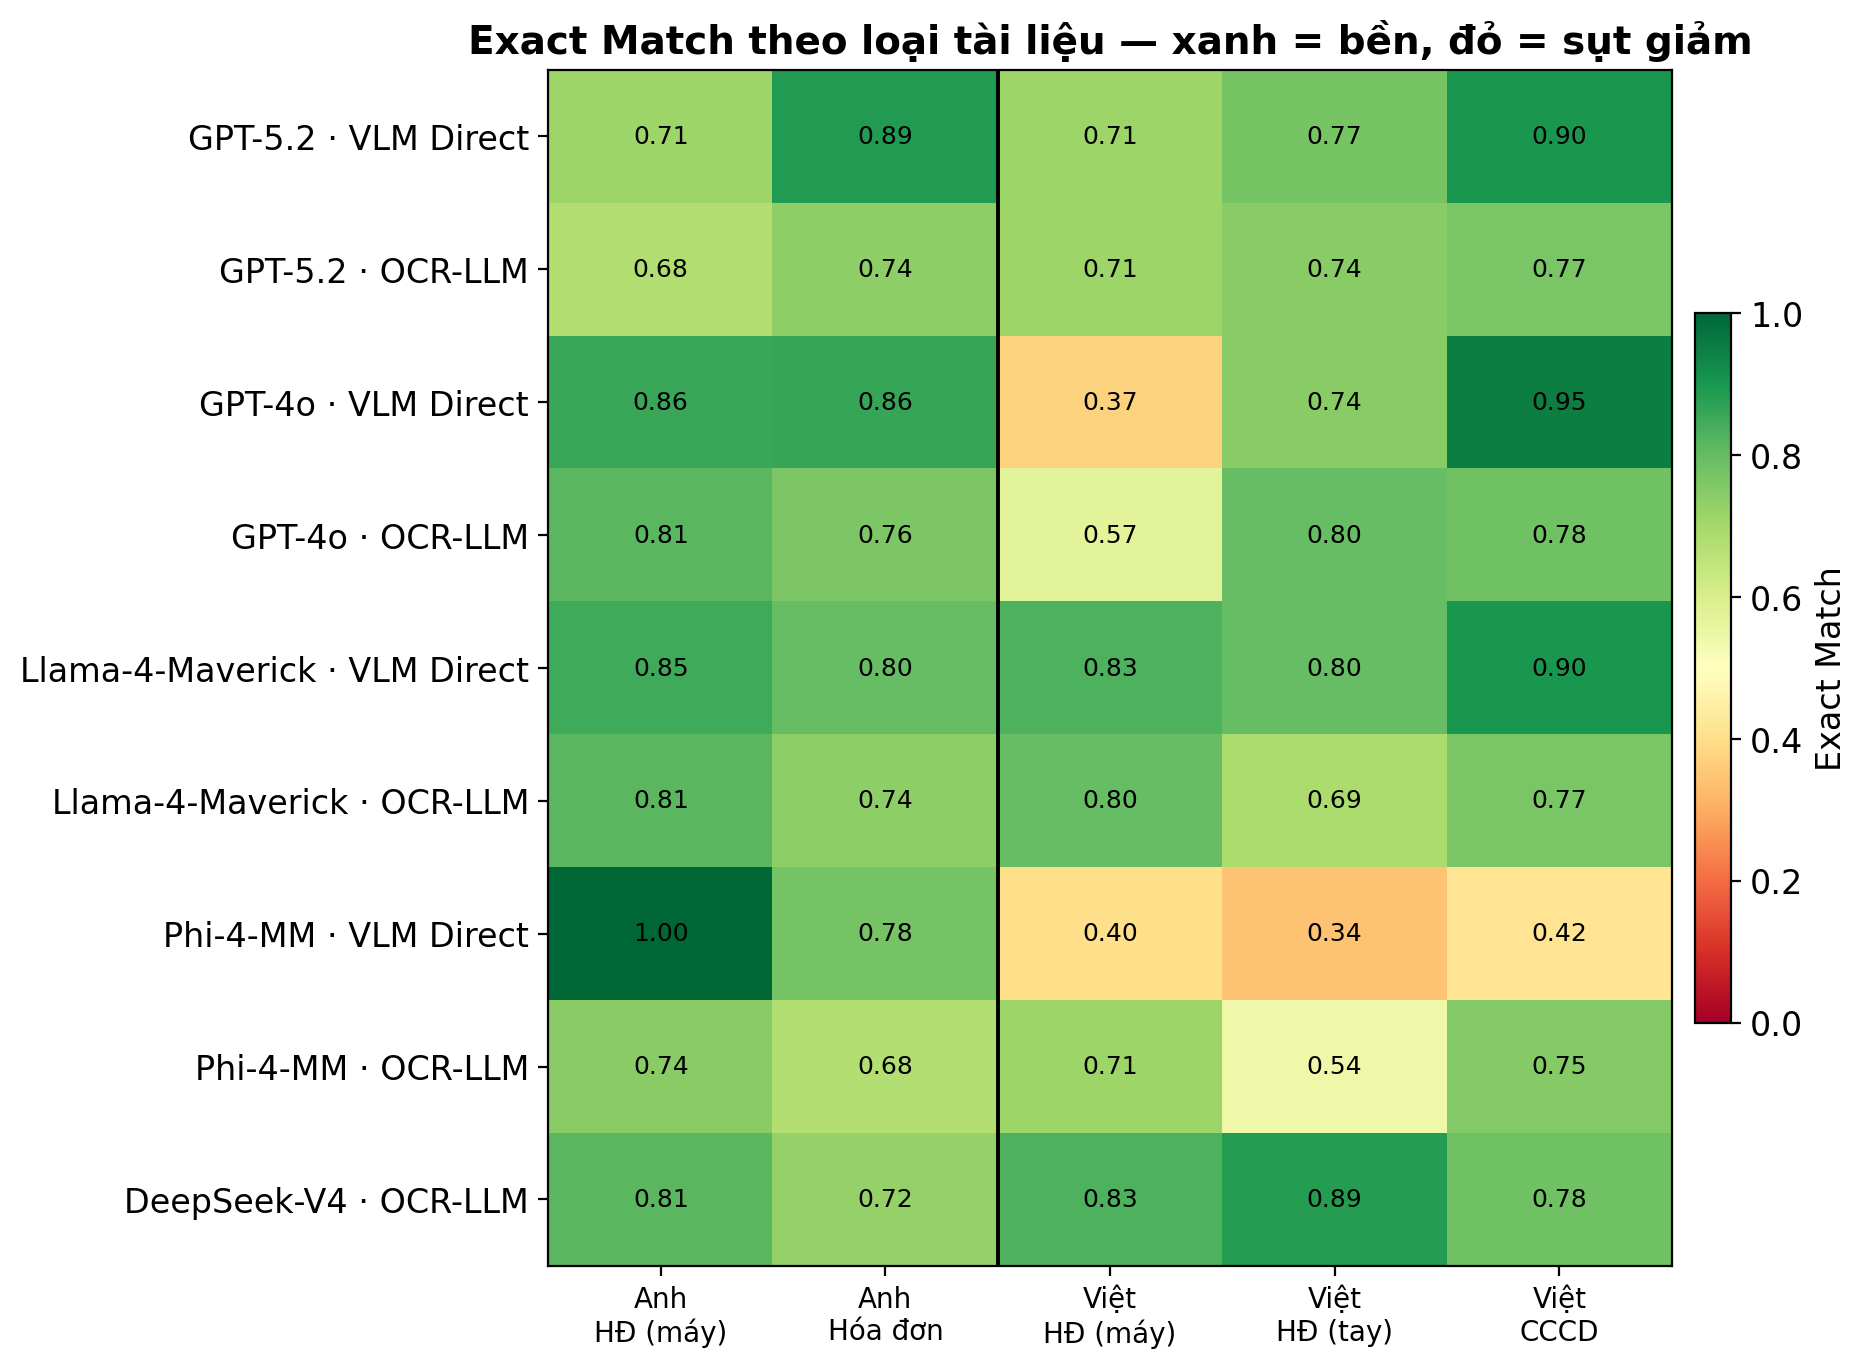
\includegraphics[width=0.85\linewidth]{Images/fig_robustness_distribution.png}
    \caption{Bản đồ nhiệt Exact Match theo từng tập con dữ liệu (ngôn ngữ $\times$ loại tài liệu)}
    \label{fig:robustness_heatmap}
\end{figure}

\subsection{Kết quả theo dạng văn bản}\label{sec:results_typed_handwritten}

Hình~\ref{fig:robustness_drop} biểu diễn mức sụt giảm EM khi chuyển từ văn bản đánh máy sang viết tay và từ tiếng Anh sang tiếng Việt trên loại tài liệu hợp đồng. Đa số mô hình đều giảm độ chính xác trên văn bản viết tay so với đánh máy, song quy trình OCR-LLM nhìn chung ổn định hơn VLM Direct trên hợp đồng viết tay tiếng Việt. Điều này cho phép kết luận rằng tính bền vững không tỉ lệ thuận với độ chính xác trung bình: một mô hình có điểm tiếng Anh rất cao vẫn có thể kém tin cậy khi áp dụng cho dữ liệu thực tế đa ngôn ngữ và viết tay.

\begin{figure}[H]
    \centering
    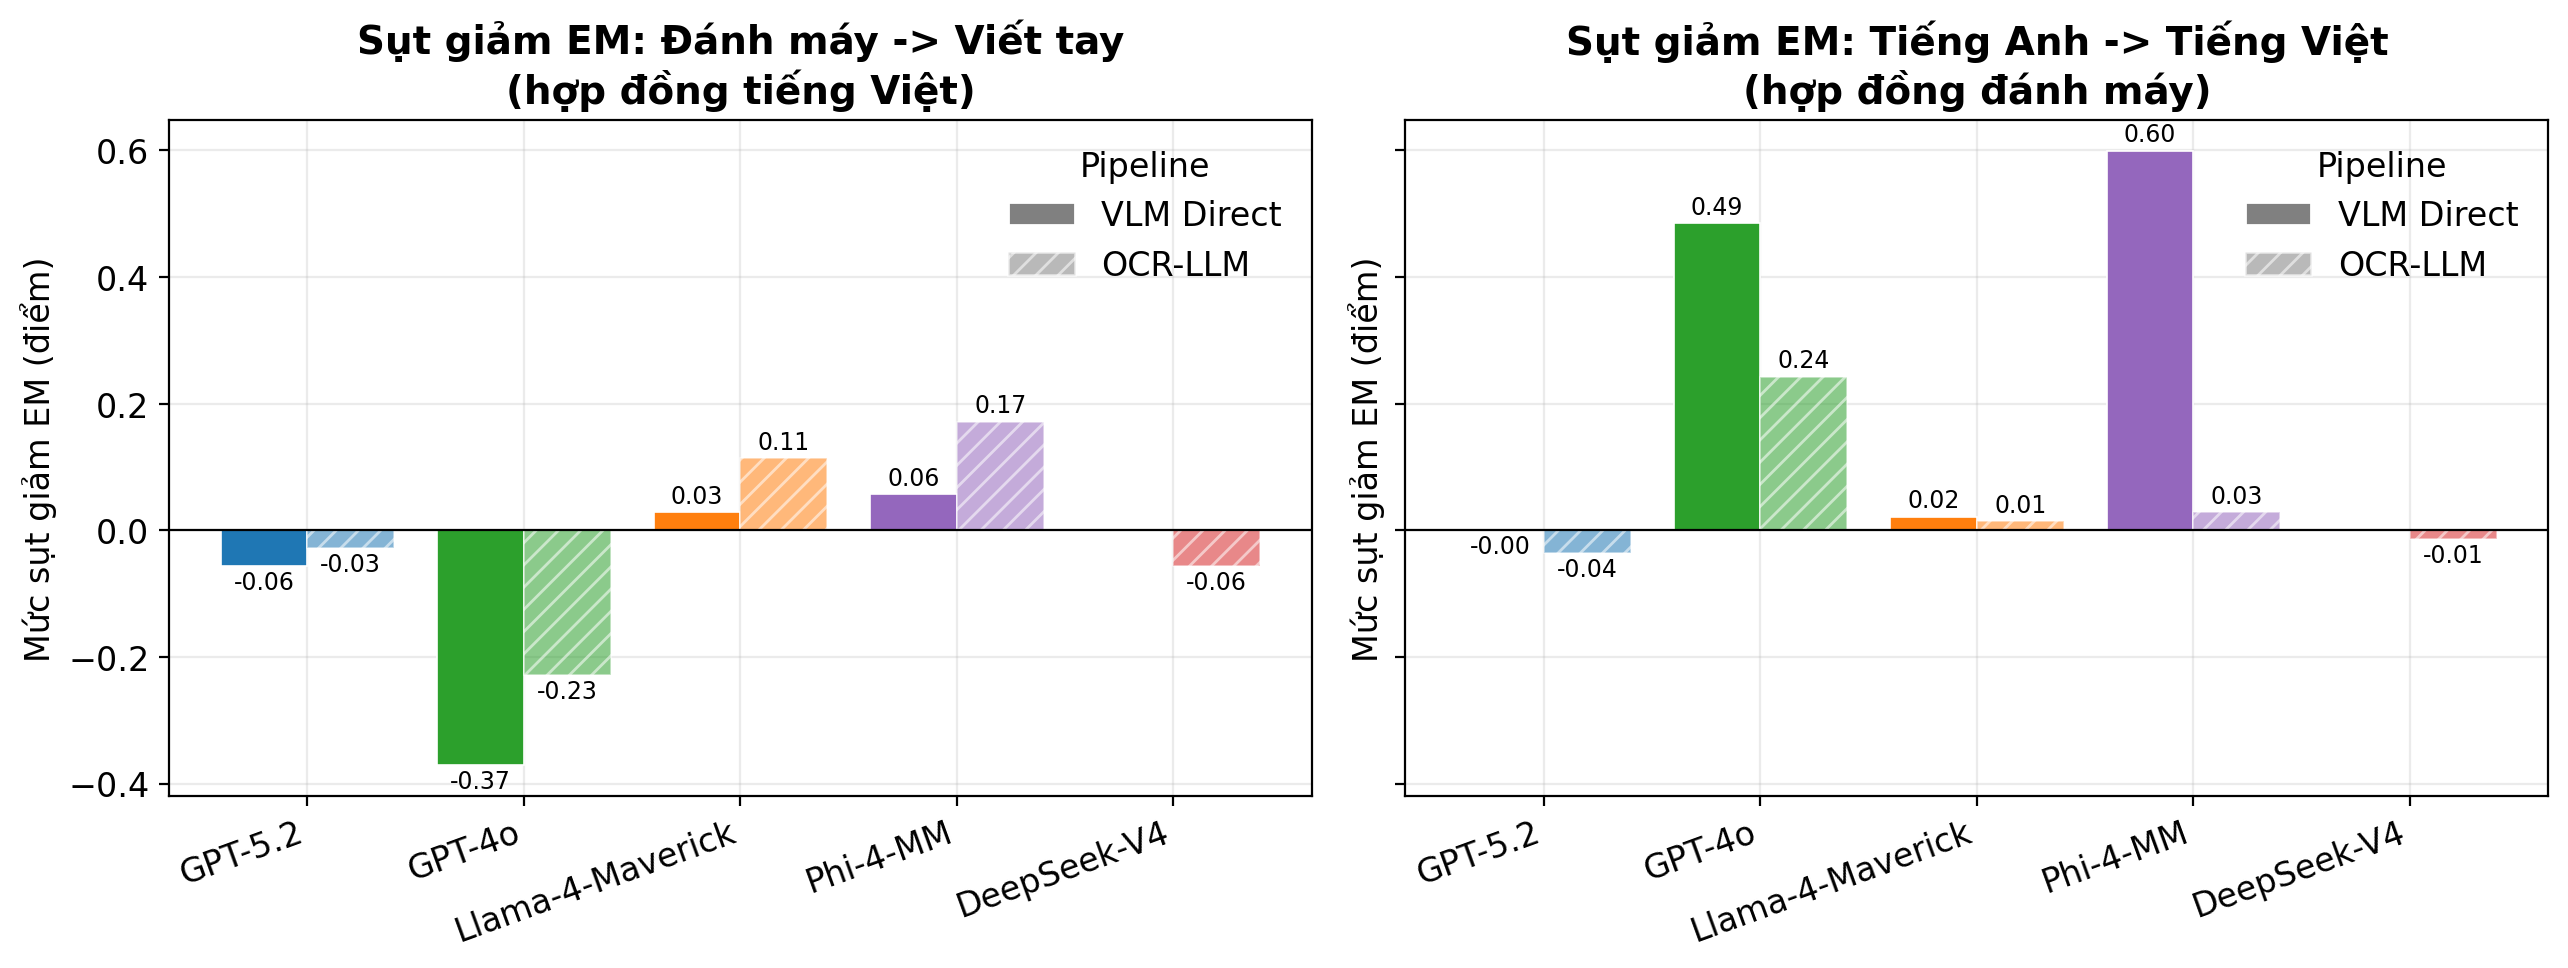
\includegraphics[width=\linewidth]{Images/fig_robustness_drop.png}
    \caption{Mức sụt giảm Exact Match theo dạng văn bản và theo ngôn ngữ}
    \label{fig:robustness_drop}
\end{figure}

\subsection{So sánh hiệu quả và chi phí}\label{sec:results_efficiency}

Về độ trễ, Llama-4-Maverick (VLM Direct) xử lý nhanh nhất với 1,76 giây mỗi tài liệu, trong khi Phi-4-MM (VLM Direct) chậm nhất với 12,55 giây, như thể hiện ở Hình~\ref{fig:efficiency_latency}. Về lượng token tiêu thụ, cấu hình OCR-LLM của Llama-4-Maverick tiết kiệm nhất với khoảng 751 token mỗi tài liệu, còn Phi-4-MM (VLM Direct) tiêu tốn nhiều nhất với khoảng 3.127 token, như minh họa ở Hình~\ref{fig:efficiency_tokens}. Về chi phí ước tính, các mô hình nhỏ có lợi thế rõ rệt khi Phi-4-MM (OCR-LLM) chỉ tốn khoảng 0,08 USD cho 1000 tài liệu, trong khi GPT-5.2 (VLM Direct) tốn tới 6,66 USD do đơn giá token cao, như thể hiện ở Hình~\ref{fig:efficiency_cost}.

\begin{figure}[H]
    \centering
    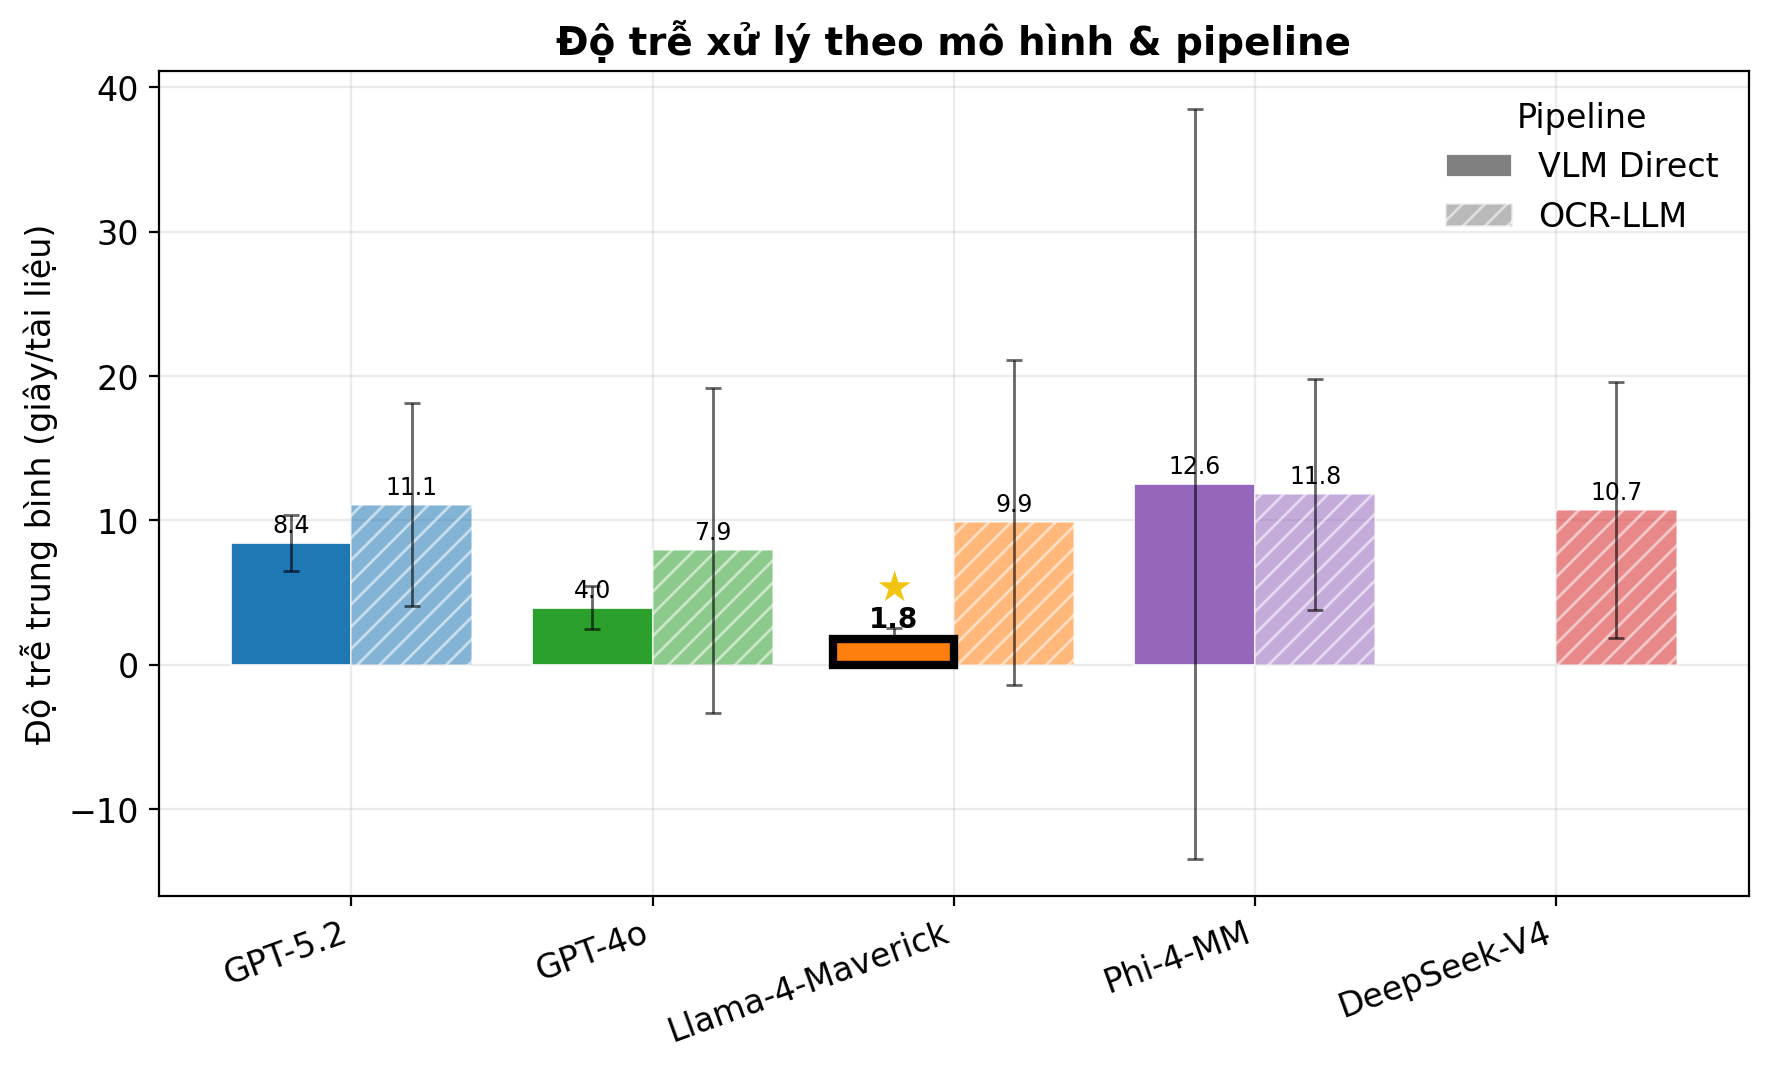
\includegraphics[width=0.8\linewidth]{Images/fig_efficiency_latency.png}
    \caption{Độ trễ xử lý theo mô hình và pipeline}
    \label{fig:efficiency_latency}
\end{figure}

\begin{figure}[H]
    \centering
    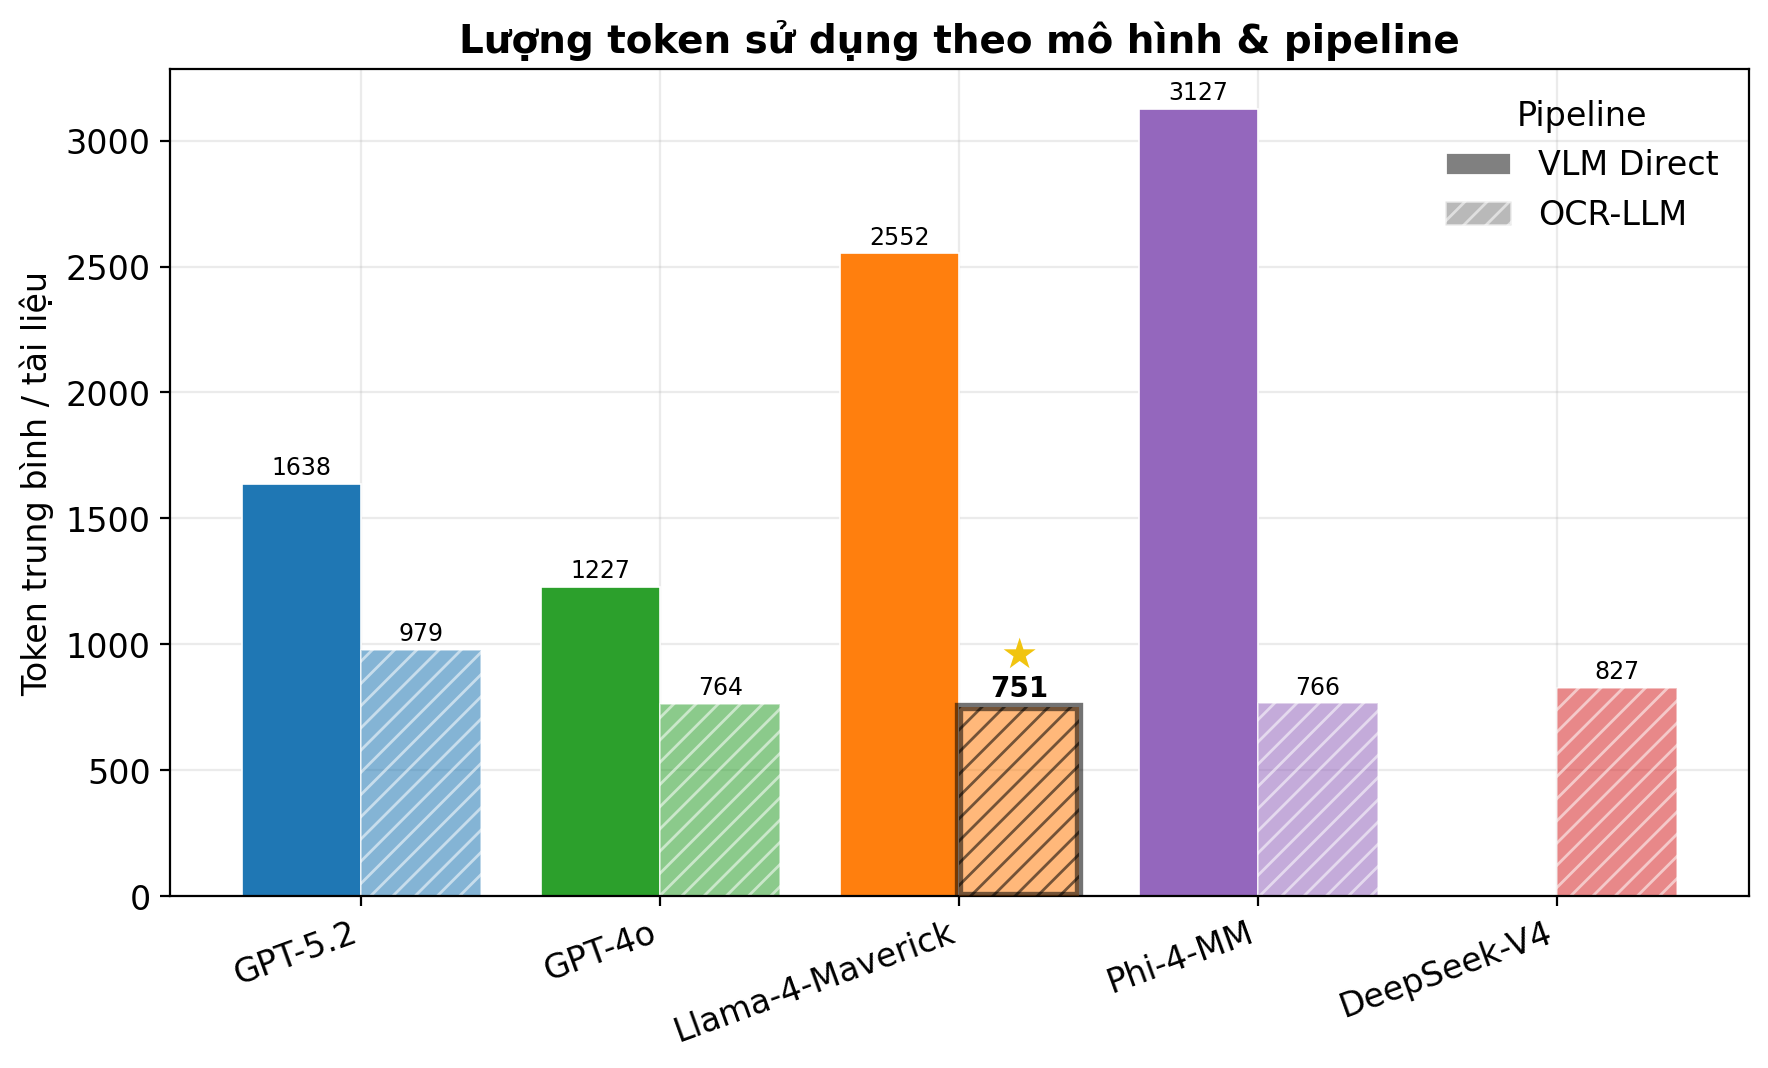
\includegraphics[width=0.8\linewidth]{Images/fig_efficiency_tokens.png}
    \caption{Lượng token sử dụng theo mô hình và pipeline}
    \label{fig:efficiency_tokens}
\end{figure}

\begin{figure}[H]
    \centering
    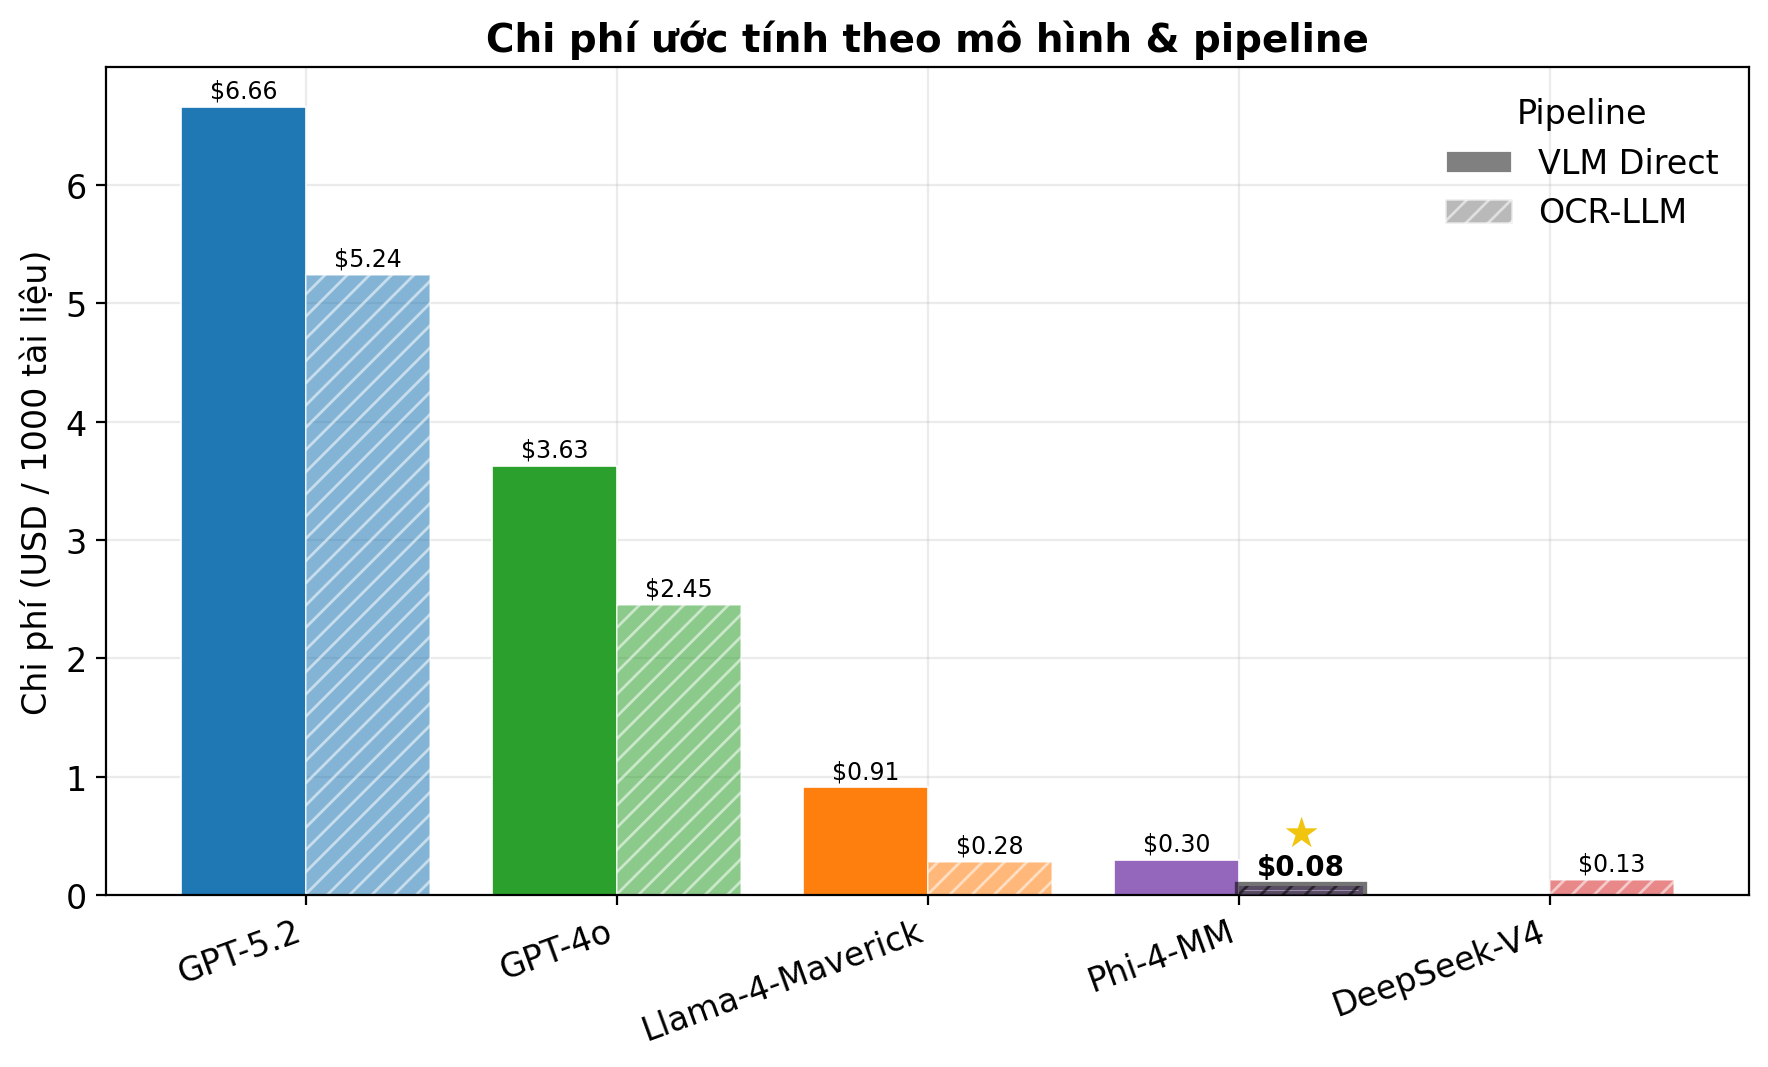
\includegraphics[width=0.8\linewidth]{Images/fig_efficiency_cost.png}
    \caption{Chi phí ước tính theo mô hình và pipeline}
    \label{fig:efficiency_cost}
\end{figure}

Có thể nhận thấy rằng chiến lược VLM Direct rút ngắn độ trễ đối với các mô hình thị giác mạnh nhờ loại bỏ bước OCR trung gian, nhưng không bảo đảm chi phí thấp hơn, vì chi phí phụ thuộc chủ yếu vào đơn giá token của từng nhà cung cấp.

\subsection{Độ tin cậy}\label{sec:results_reliability}

Trên thước đo tỉ lệ tuân thủ schema, hầu hết các cấu hình đều đạt xấp xỉ 100\%, chứng tỏ các mô hình tuân thủ tốt định dạng JSON phẳng được yêu cầu, như minh họa ở Hình~\ref{fig:reliability}. Tuy nhiên, tỉ lệ hallucination, tức hiện tượng mô hình tự sinh giá trị cho những trường vốn rỗng trong nhãn chuẩn, phân hóa mạnh giữa các mô hình. GPT-5.2 đạt mức 0\% ở cả hai pipeline, thể hiện tính kỷ luật cao nhất, trong khi Phi-4-MM (VLM Direct) lên tới 26,8\%, cho thấy xu hướng sinh khống thông tin nghiêm trọng khi xử lý trực tiếp trên ảnh. Kết quả này cho thấy độ tin cậy là tiêu chí cần được xét song song với độ chính xác, bởi một mô hình có thể đạt EM khá nhưng vẫn rủi ro cao khi triển khai thực tế nếu thường xuyên bịa giá trị cho các trường không tồn tại.

\begin{figure}[H]
    \centering
    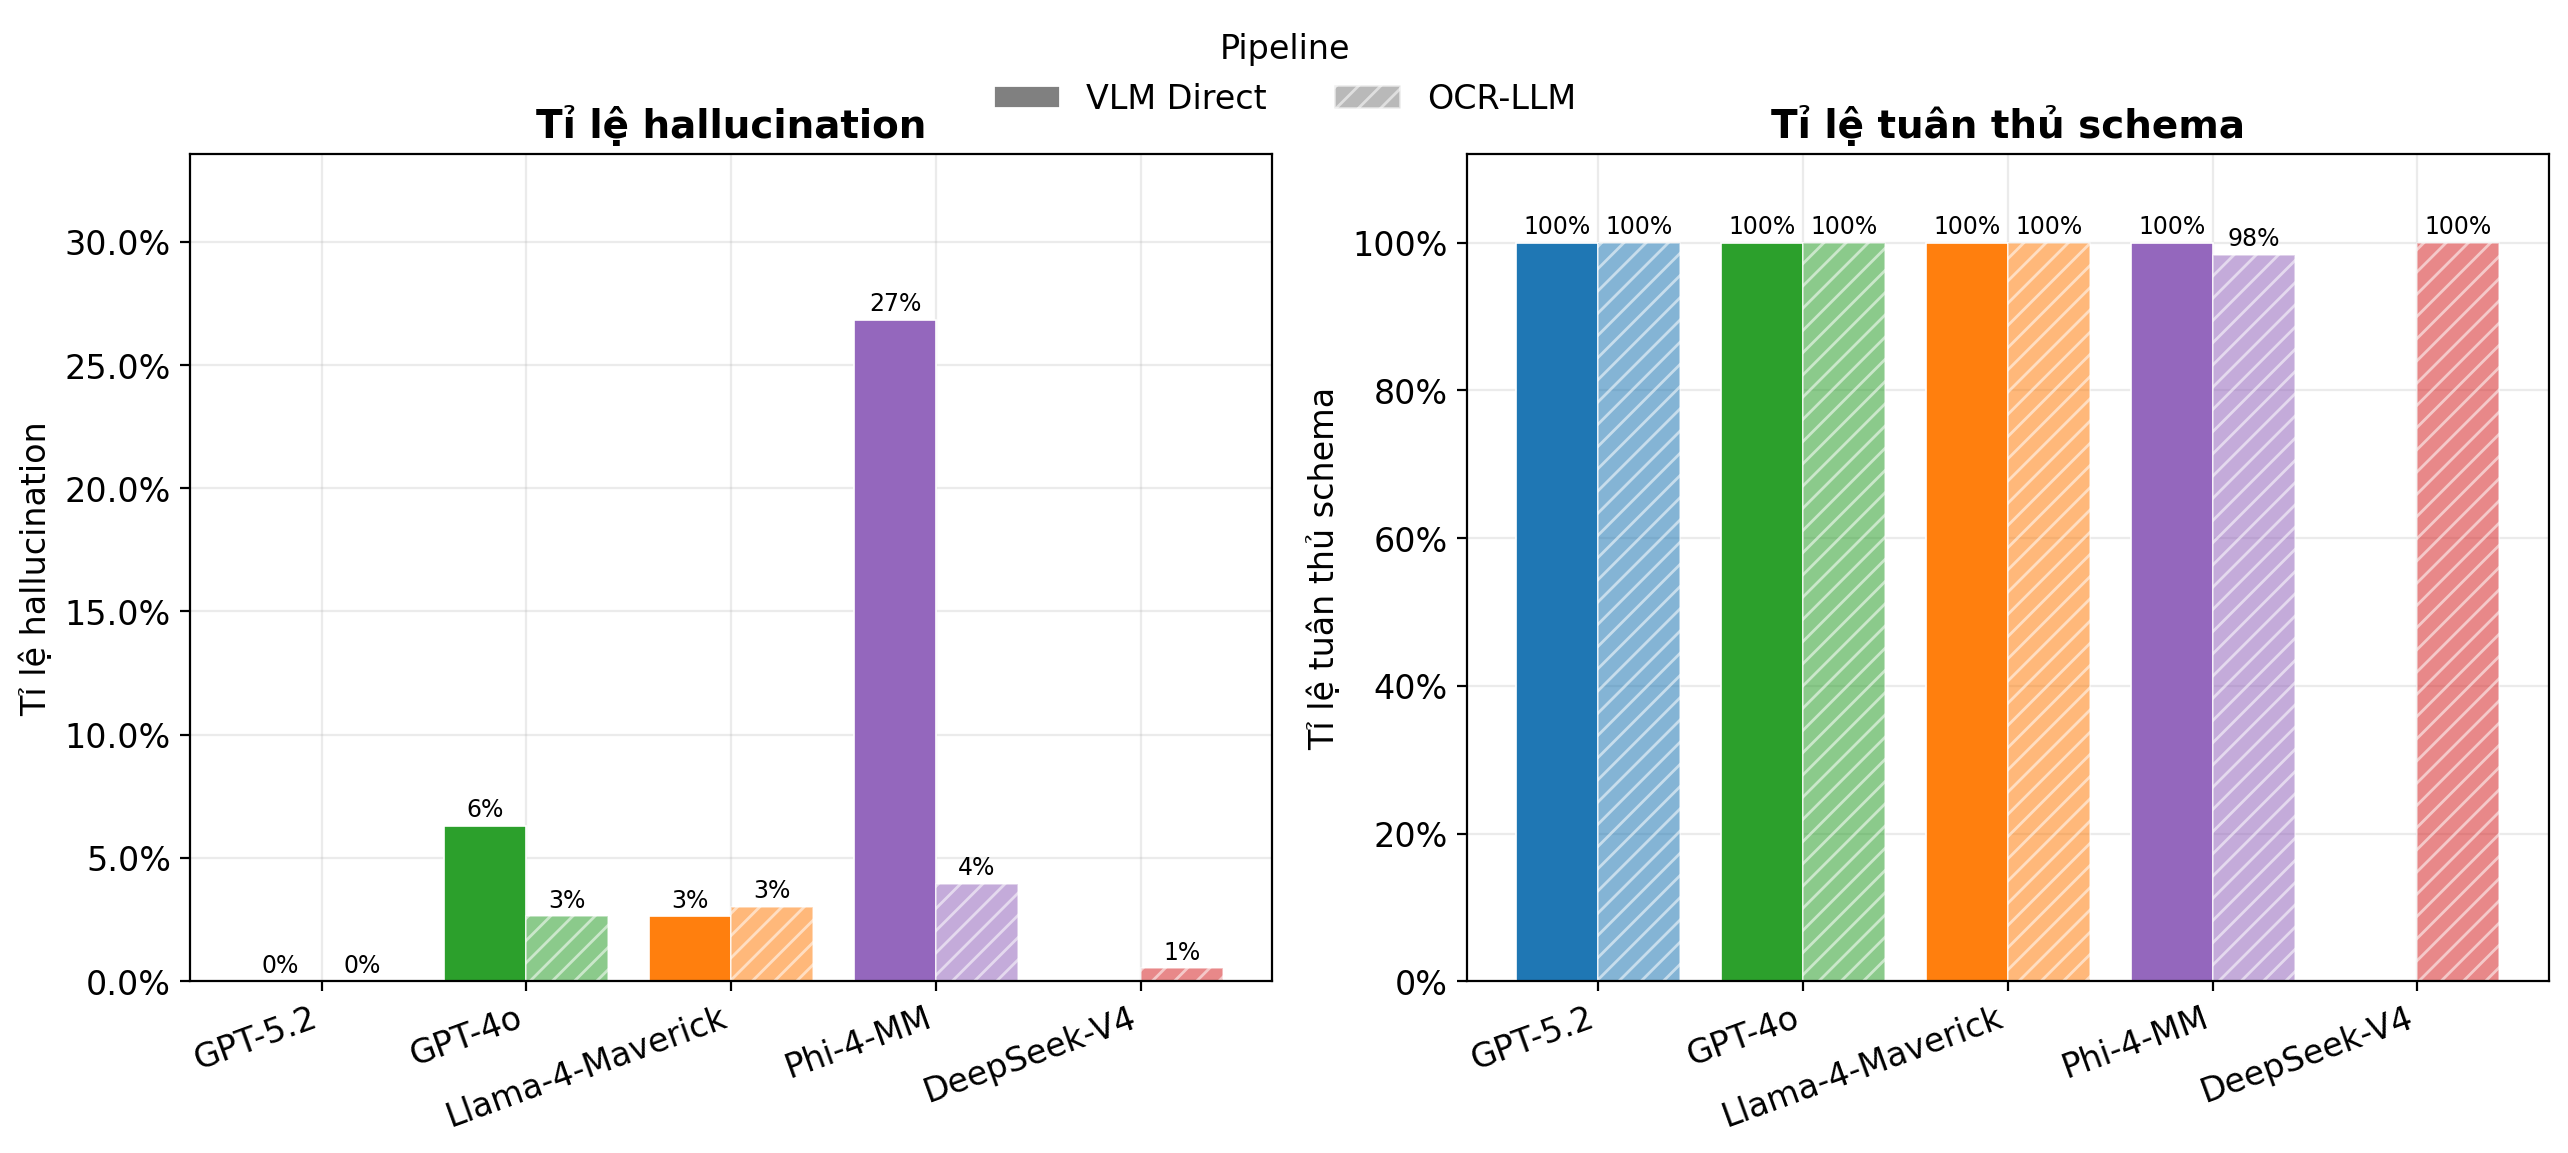
\includegraphics[width=\linewidth]{Images/fig_reliability.png}
    \caption{Tỉ lệ hallucination và tỉ lệ tuân thủ schema theo mô hình và pipeline}
    \label{fig:reliability}
\end{figure}

Tổng hợp cả bốn chiều đánh giá, Llama-4-Maverick (VLM Direct) là cấu hình cân bằng tốt nhất khi đồng thời dẫn đầu về độ chính xác, độ trễ thấp, chi phí hợp lý và tỉ lệ hallucination thấp. Đối với tài liệu tiếng Việt, quy trình OCR-LLM kết hợp DeepSeek-V4 là lựa chọn đáng cân nhắc nhờ độ bền vững vượt trội. Kết quả này cho phép trả lời mục tiêu so sánh của đề tài: chiến lược VLM Direct phù hợp với tài liệu tiếng Anh đánh máy và yêu cầu độ trễ thấp, còn OCR-LLM giữ vai trò quan trọng đối với tài liệu tiếng Việt, viết tay, hoặc khi sử dụng các mô hình ngôn ngữ thuần văn bản.

\section{Thiết kế hệ thống trích xuất dữ liệu (Mockup)}\label{sec:system_design}


Nhằm minh họa khả năng ứng dụng thực tiễn của các kết quả nghiên cứu, tác giả
thiết kế một giao diện nguyên mẫu tổ chức luồng trích xuất dữ liệu có cấu trúc
từ tài liệu ảnh thành năm bước tuần tự: tải tài liệu, định nghĩa lược đồ, lựa
chọn pipeline và mô hình, theo dõi tiến trình xử lý, và xem kết quả đầu ra.
Thiết kế này cho phép người dùng trải nghiệm toàn bộ quy trình mà không cần
kiến thức lập trình, đồng thời thể hiện cách các thành phần nghiên cứu của
luận văn được gắn kết thành một sản phẩm hoàn chỉnh.

Điểm xuất phát của hệ thống là màn hình tải tài liệu, hỗ trợ các định dạng
PDF, JPG, PNG và TIFF thông qua thao tác kéo-thả.

\begin{figure}[H]
    \centering
    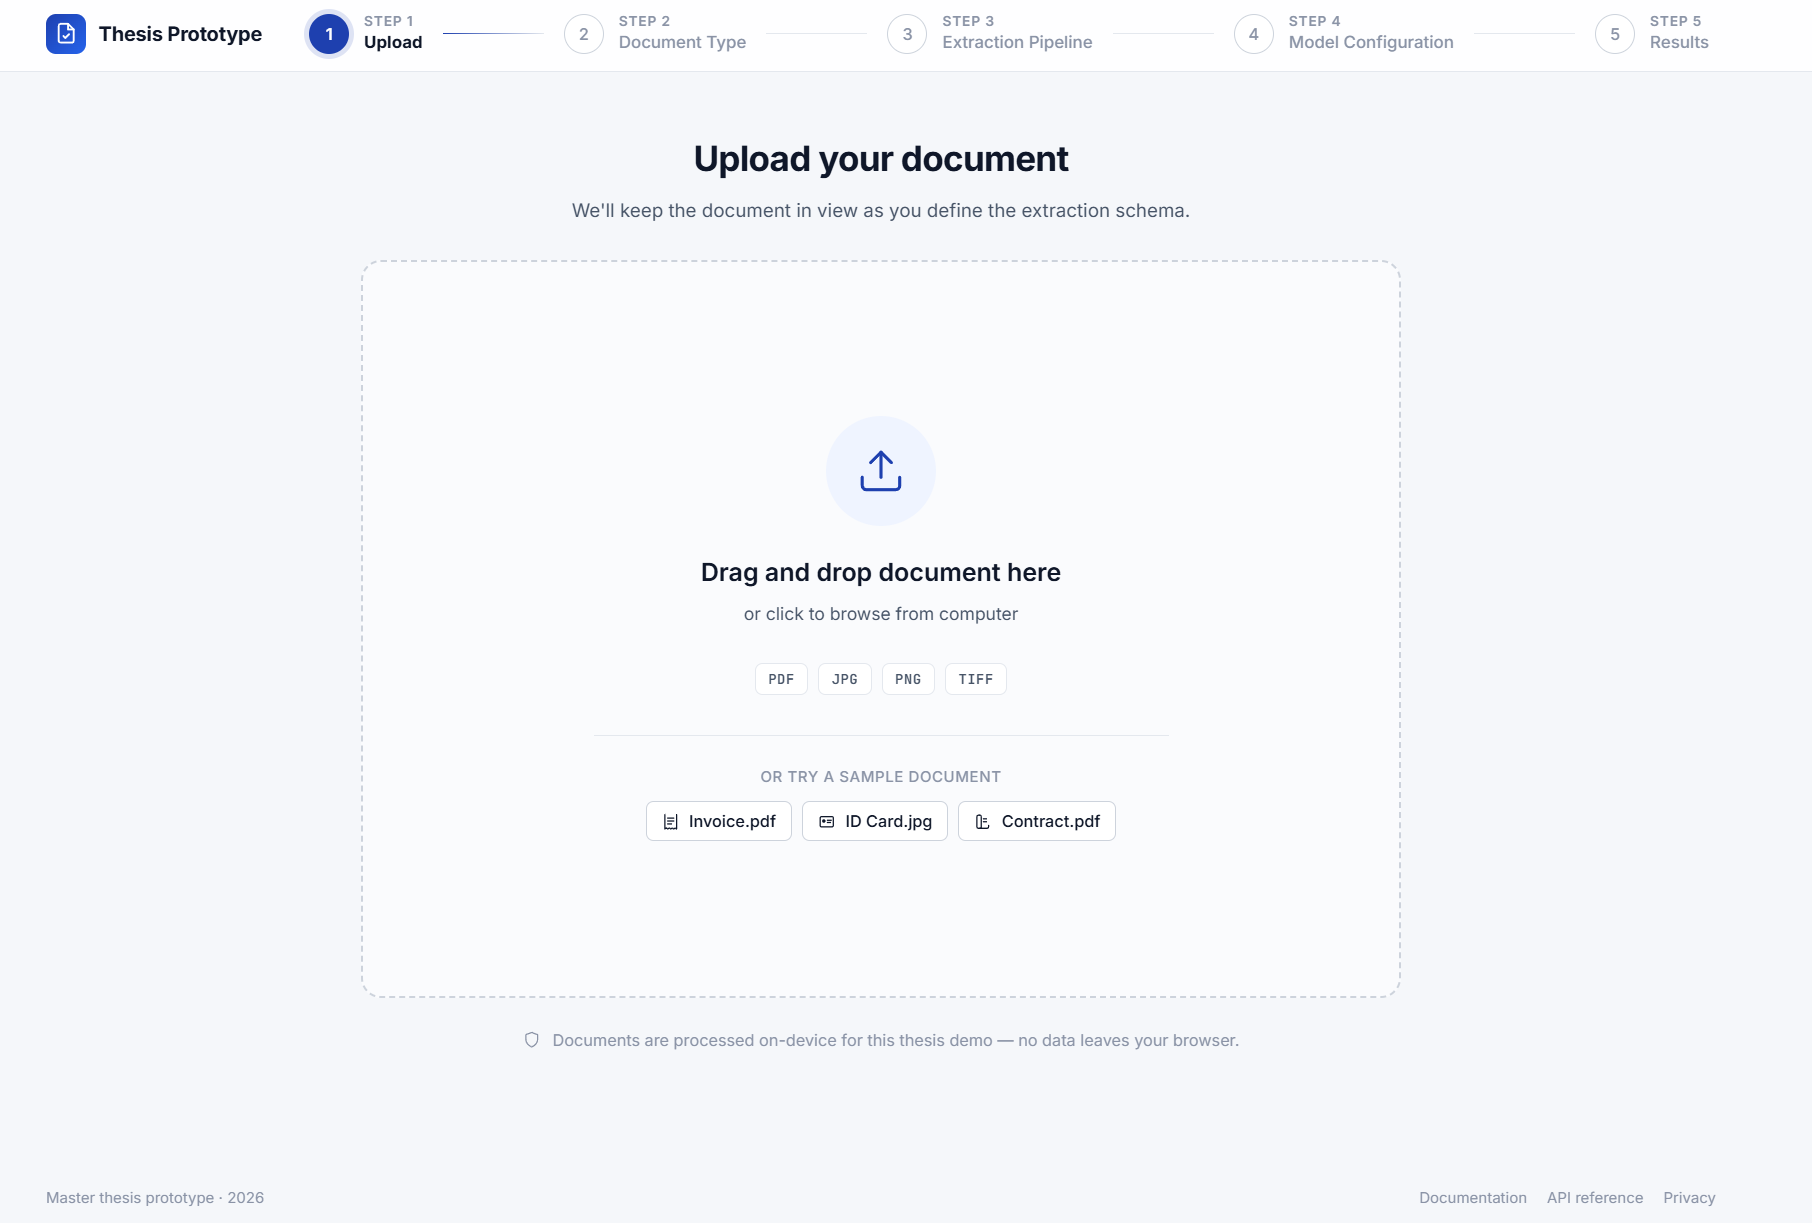
\includegraphics[width=0.85\linewidth]{Images/Mockup_Step1.png}
    \caption{Giao diện tải tài liệu đầu vào}
    \label{fig:mockup_step1}
\end{figure}

Sau khi tải tài liệu, người dùng khai báo lược đồ trích xuất gồm tên các
trường thông tin và mô tả ngữ nghĩa tương ứng, phản ánh cơ chế truyền đạt kỳ
vọng cho mô hình thông qua prompt có cấu trúc mà luận văn đã sử dụng.

\begin{figure}[H]
    \centering
    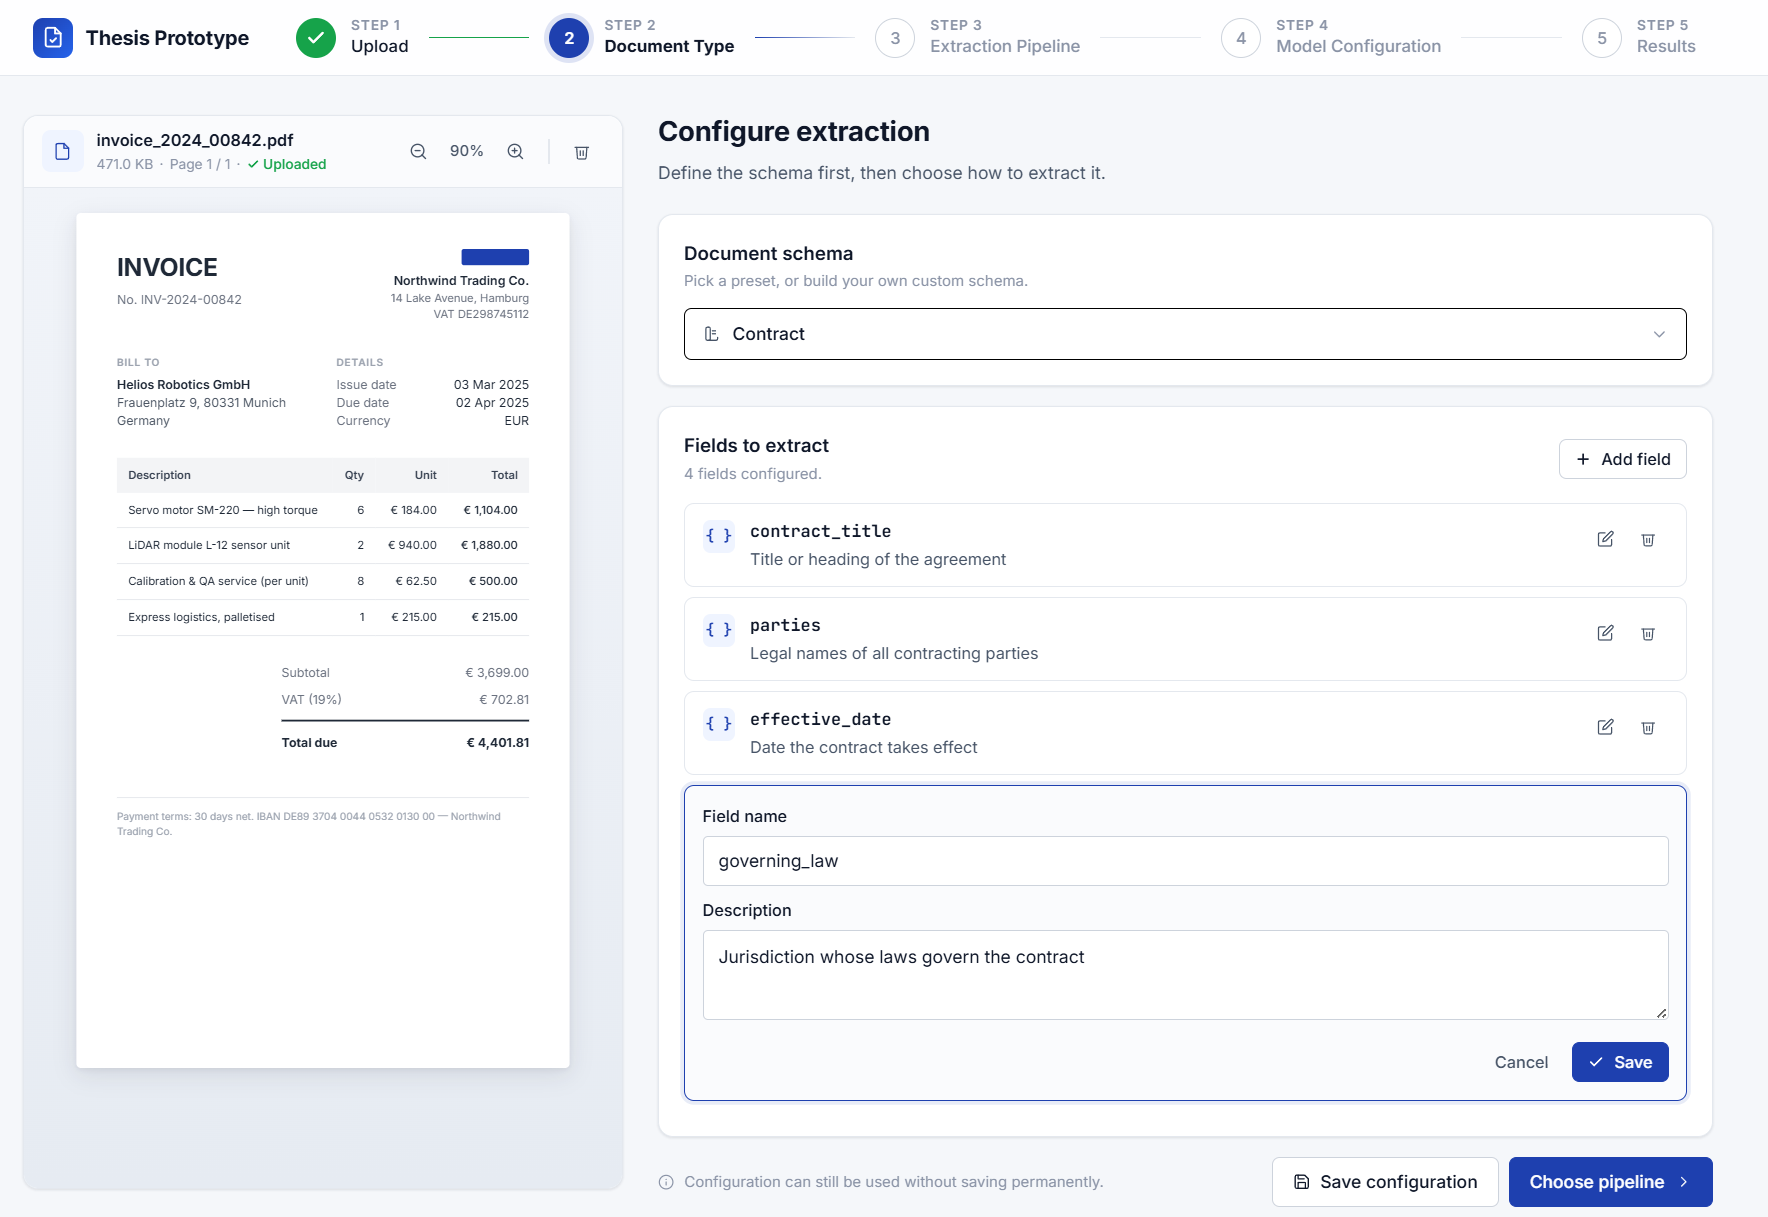
\includegraphics[width=0.85\linewidth]{Images/Mockup_Step2.png}
    \caption{Giao diện định nghĩa lược đồ trích xuất}
    \label{fig:mockup_step2}
\end{figure}

Tiếp theo, người dùng lựa chọn kiến trúc pipeline (VLM trực tiếp hoặc
OCR-LLM) và mô hình xử lý phù hợp với đặc điểm của tài liệu, với gợi ý ngắn
về ưu điểm của từng phương án.

\begin{figure}[H]
    \centering
    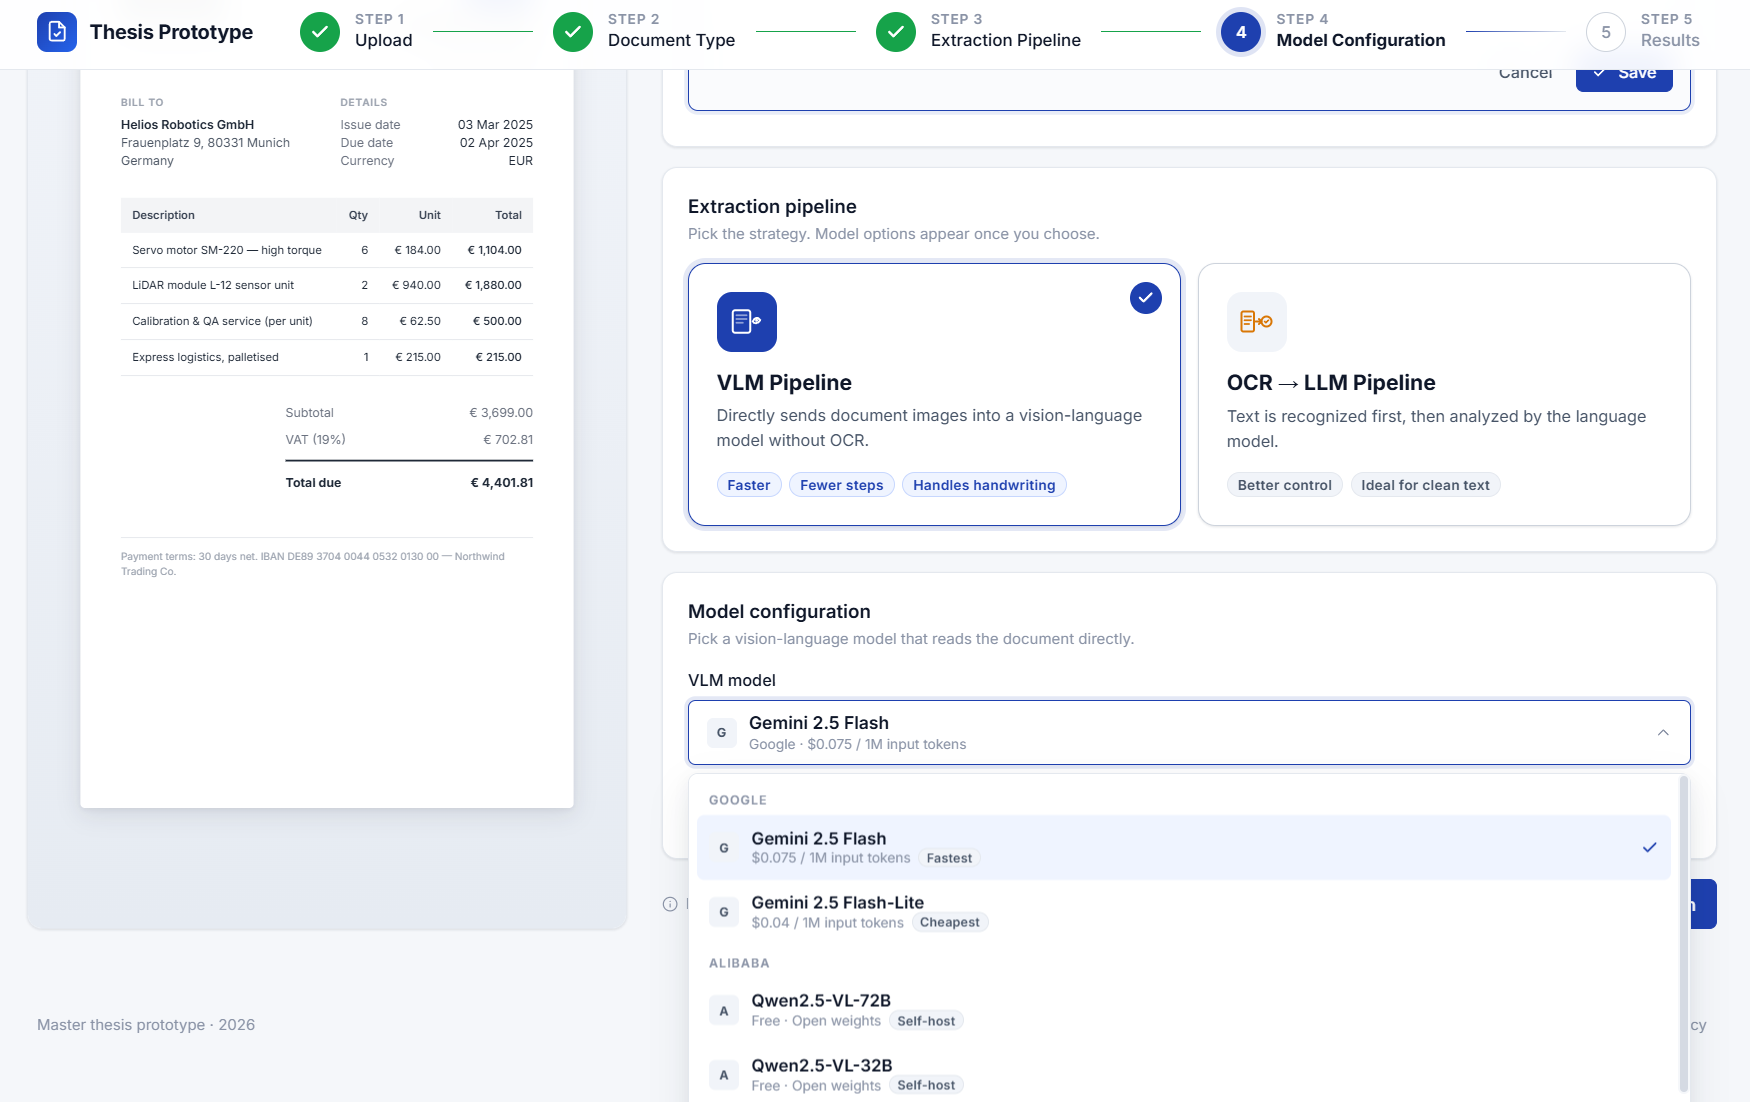
\includegraphics[width=0.85\linewidth]{Images/Mockup_Step3.png}
    \caption{Giao diện lựa chọn pipeline và mô hình}
    \label{fig:mockup_step3}
\end{figure}

Quá trình xử lý được hiển thị minh bạch qua từng giai đoạn, giúp người dùng
nắm được thứ tự thực thi thực sự bên trong hệ thống thay vì chỉ chờ đợi mà
không có phản hồi.

\begin{figure}[H]
    \centering
    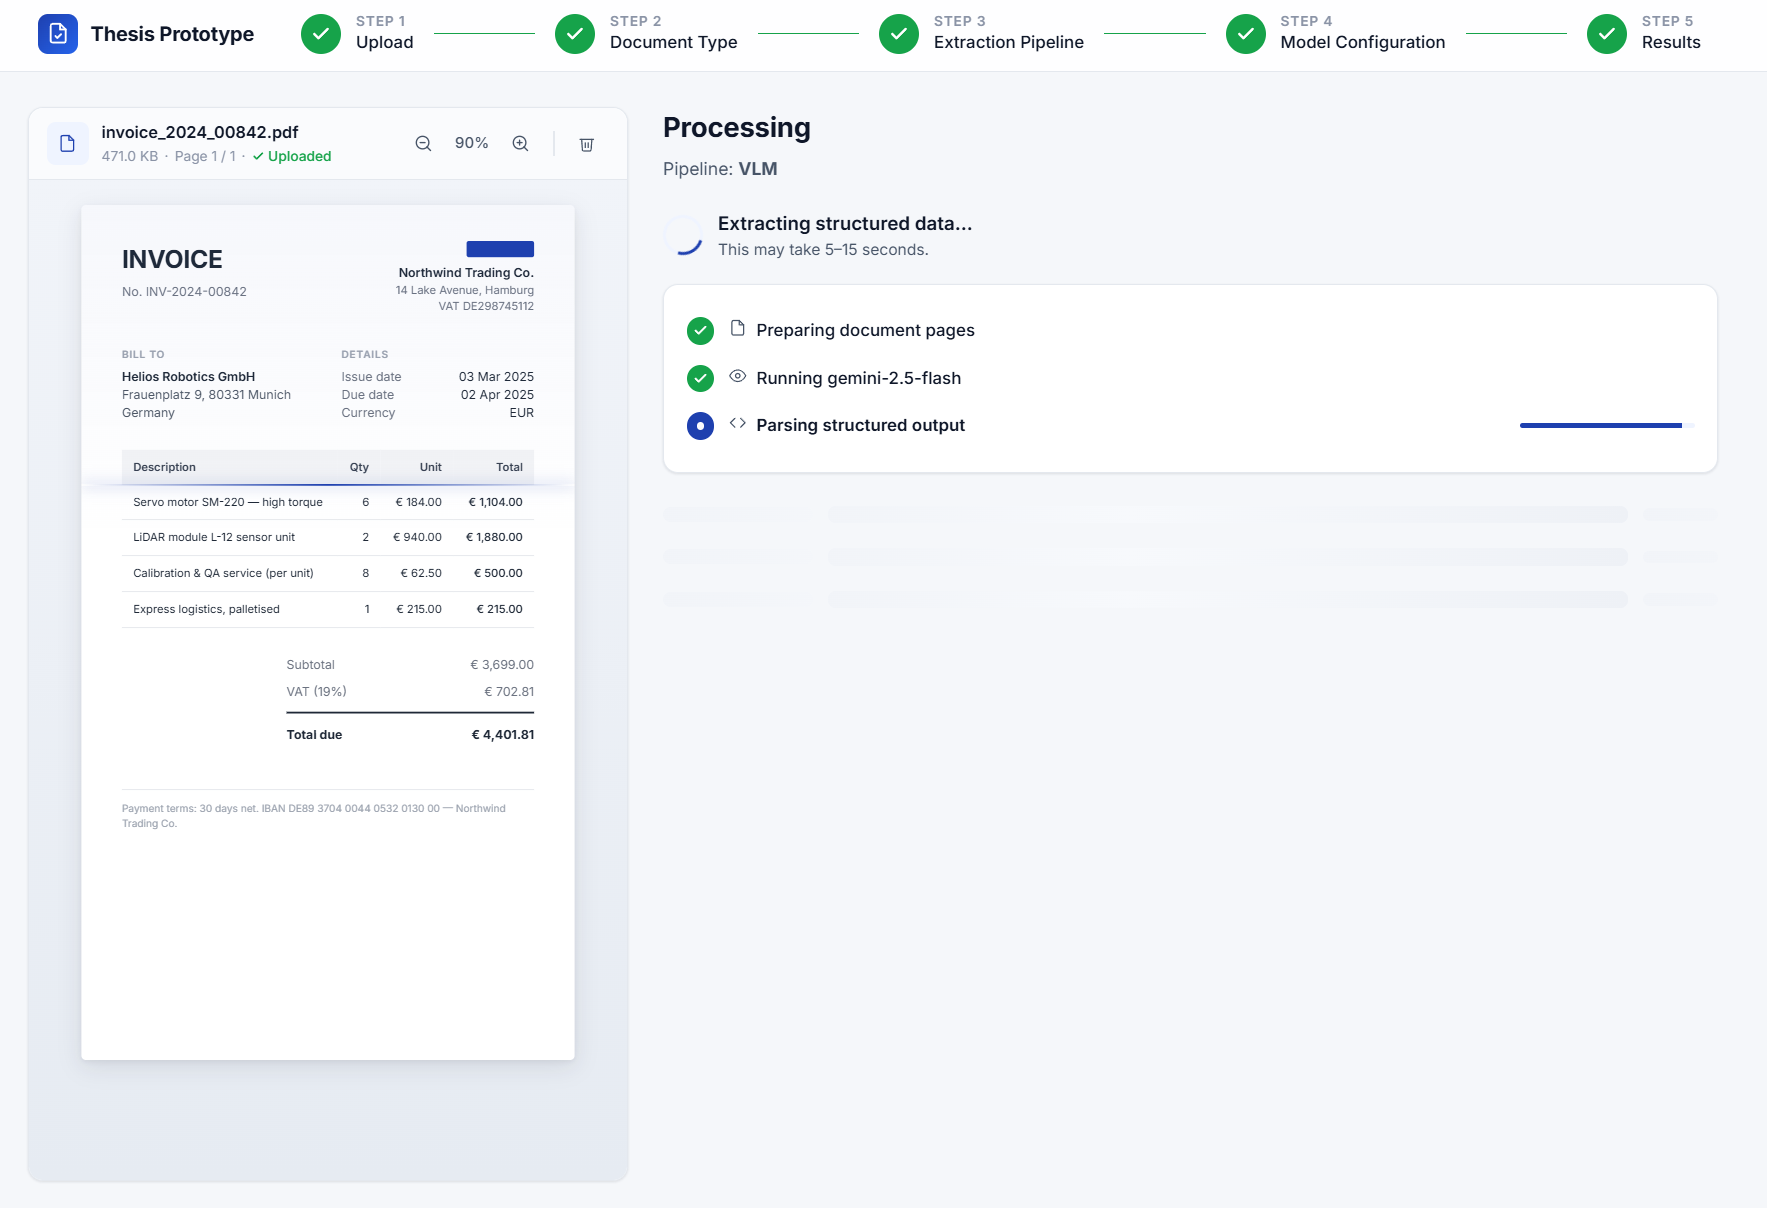
\includegraphics[width=0.85\linewidth]{Images/Mockup_Step4.png}
    \caption{Giao diện theo dõi tiến trình xử lý}
    \label{fig:mockup_step4}
\end{figure}

Kết quả trích xuất được trình bày ở hai chế độ, dạng bảng trực quan và dạng
JSON thô, kèm các chỉ số hiệu năng thực tế của phiên xử lý bao gồm độ trễ,
số token tiêu thụ và chi phí ước tính.

\begin{figure}[H]
    \centering
    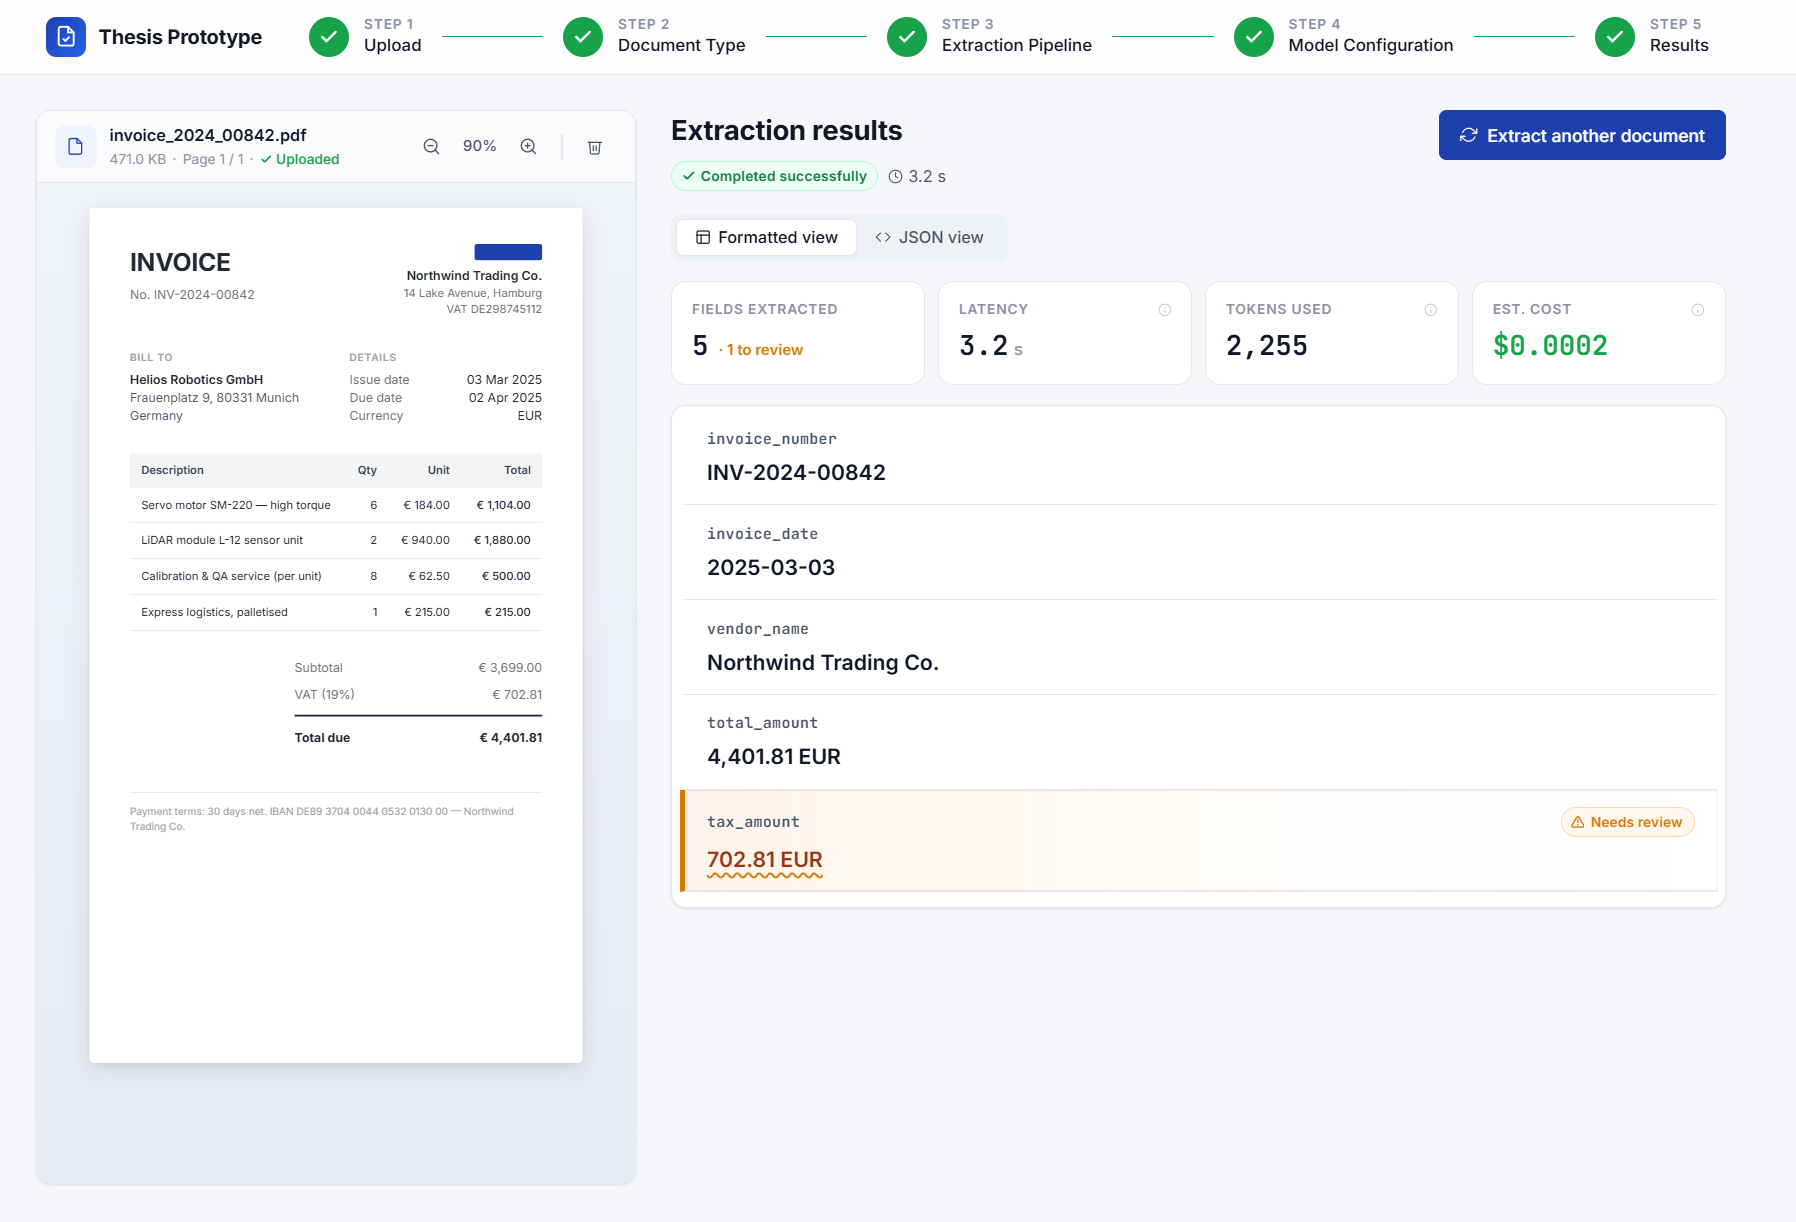
\includegraphics[width=0.85\linewidth]{Images/Mockup_Step5.png}
    \caption{Giao diện kết quả trích xuất và chỉ số hiệu năng}
    \label{fig:mockup_step5}
\end{figure}

\clearpage

% ============================================================
% CHƯƠNG 5 — KẾT LUẬN
% ============================================================
\chapter{Kết luận}

Nội dung chương này khái quát lại những kết quả đã đạt được trong quá trình thực hiện đề tài, nhận xét các hạn chế còn tồn tại và đề xuất hướng phát triển trong tương lai.

\section{Nhận xét và tổng kết}\label{sec:conclusion}

Đề tài đã xây dựng và đánh giá toàn diện hai hướng tiếp cận trích xuất dữ liệu có cấu trúc từ tài liệu trên một benchmark gồm 60 mẫu trải rộng hai ngôn ngữ (tiếng Anh và tiếng Việt), ba loại tài liệu (hóa đơn, căn cước công dân và hợp đồng) và hai dạng văn bản (đánh máy và viết tay). Tổng cộng 540 lượt trích xuất được thực hiện trên 5 mô hình qua hai pipeline, tạo thành bộ kết quả benchmark có thể tái lập, phục vụ so sánh định lượng giữa VLM Direct (Pipeline A) và OCR-LLM (Pipeline B) theo bốn chiều: độ chính xác, độ bền vững, hiệu quả và độ tin cậy.

\begin{itemize}
    \item \textbf{Về độ chính xác tổng thể:} Trong phần lớn cấu hình, Pipeline A (VLM Direct) đạt Exact Match và Token-F1 cao hơn Pipeline B (OCR-LLM). Llama-4-Maverick kết hợp VLM Direct dẫn đầu toàn bảng với EM 83,6\% và Token-F1 92,3\%, đồng thời có độ trễ thấp nhất ở mức 1,76 giây mỗi tài liệu. DeepSeek-V4 dẫn đầu nhóm OCR-LLM với EM 78,6\%, cho thấy mô hình ngôn ngữ thuần văn bản vẫn cạnh tranh khi văn bản OCR đủ chất lượng.

    \item \textbf{Về độ bền vững theo ngôn ngữ:} Phi-4-Multimodal (VLM Direct) cho thấy mức sụt giảm nghiêm trọng khi chuyển từ tiếng Anh sang tiếng Việt (EM từ 88,8\% xuống 39,4\%), trong khi DeepSeek-V4 (OCR-LLM) duy trì được độ bền vững tốt nhất, thậm chí đạt EM tiếng Việt (82,0\%) cao hơn tiếng Anh (77,0\%), nhờ ưu thế của OCR engine chuyên biệt kết hợp mô hình ngôn ngữ lớn.

    \item \textbf{Về hiệu quả và chi phí:} Chi phí triển khai không tỉ lệ thuận với độ chính xác. Phi-4-Multimodal (OCR-LLM) là cấu hình rẻ nhất ở mức 0,08 USD/1000 tài liệu, trong khi GPT-5.2 (VLM Direct) đắt nhất ở 6,66 USD; Llama-4-Maverick (VLM Direct) đạt điểm cân bằng tốt giữa độ chính xác, độ trễ và chi phí.

    \item \textbf{Về độ tin cậy:} Tỉ lệ tuân thủ schema đạt gần 100\% trên toàn bộ cấu hình. Tỉ lệ hallucination phân hóa mạnh: GPT-5.2 đạt 0\% ở cả hai pipeline, trong khi Phi-4-Multimodal (VLM Direct) lên tới 26,8\%.
\end{itemize}

Kết quả thực nghiệm xác nhận rằng lựa chọn pipeline tối ưu phụ thuộc vào bối cảnh sử dụng: VLM Direct phù hợp với tài liệu tiếng Anh đánh máy và hệ thống yêu cầu độ trễ thấp; OCR-LLM quan trọng với tài liệu tiếng Việt, văn bản viết tay, hoặc khi cần kết hợp mô hình ngôn ngữ thuần văn bản chi phí thấp. Chi tiết kết quả được trình bày tại \hyperref[sec:results]{Mục 4.5}.

\section{Hạn chế của nghiên cứu}\label{sec:limitations}

Bên cạnh những kết quả đạt được, nghiên cứu còn một số hạn chế cần được nhìn nhận:

\begin{itemize}
    \item \textbf{Quy mô và phân bố tập benchmark còn hạn chế:} Tổng số 60 mẫu, trong đó chỉ có 5 mẫu viết tay và mỗi tập con tiếng Việt chỉ 5--10 mẫu (IdCard 10, Contract typed/handwritten mỗi loại 5); ngoài ra tiếng Anh không có mẫu căn cước công dân và tiếng Việt không có mẫu hóa đơn, khiến so sánh theo ngôn ngữ trên cùng loại tài liệu bị giới hạn. Kết quả phân tích theo ngôn ngữ và dạng văn bản vì vậy mang tính chỉ dẫn hơn là kết luận thống kê đủ mạnh.

    \item \textbf{Chỉ đánh giá theo chế độ zero-shot:} Các mô hình được đánh giá mà không thực hiện tinh chỉnh (fine-tuning) do giới hạn tài nguyên tính toán. Hiệu năng có thể cải thiện đáng kể nếu mô hình được huấn luyện thêm trên dữ liệu tài liệu tiếng Việt.

    \item \textbf{Giới hạn ở tài liệu một trang:} Toàn bộ mẫu trong benchmark đều là trang đơn. Tài liệu nhiều trang, đặc biệt hợp đồng thực tế thường dài hàng chục trang, chưa được xem xét trong phạm vi đề tài.

    \item \textbf{Chi phí đánh giá phụ thuộc vào thời điểm:} Giá API được ghi nhận tại thời điểm thực nghiệm (tháng 5/2026) và có thể thay đổi theo chính sách định giá của nhà cung cấp.

    \item \textbf{Chưa đánh giá robustness theo chất lượng ảnh có kiểm soát:} Benchmark chưa bổ sung các biến thể nhiễu có kiểm soát (mờ, chụp nghiêng, thiếu sáng) để đo đạc mức sụt giảm hiệu năng theo chất lượng ảnh đầu vào một cách hệ thống.
\end{itemize}

\section{Hướng phát triển trong tương lai}\label{sec:future_work}

Từ những hạn chế trên, tác giả đề xuất một số hướng mở rộng và cải thiện cho các nghiên cứu tiếp theo:

\begin{itemize}
    \item \textbf{Xây dựng benchmark tiếng Việt quy mô lớn hơn:} Mở rộng tập dữ liệu tiếng Việt với nhiều loại tài liệu hơn (như phiếu lương, giấy tờ hành chính, tờ khai thuế), tăng số lượng mẫu viết tay, và đa dạng hóa chất lượng ảnh đầu vào.

    \item \textbf{Tinh chỉnh mô hình trên dữ liệu tài liệu tiếng Việt:} Thử nghiệm fine-tuning các mô hình VLM mã nguồn mở (như Qwen2.5-VL hay Phi-4-Multimodal) trên tập tài liệu tiếng Việt tự thu thập, nhằm thu hẹp khoảng cách hiệu năng so với tài liệu tiếng Anh.

    \item \textbf{Tích hợp thông tin bố cục tài liệu:} Kết hợp thông tin vị trí không gian (bounding box) vào biểu diễn đầu vào, tương tự cách tiếp cận của LayoutLM~\cite{xu2020layoutlm} và LayoutLMv3~\cite{huang2022layoutlmv3}, có thể cải thiện độ chính xác trên tài liệu có cấu trúc phức tạp như bảng biểu và form nhiều cột.

    \item \textbf{Mở rộng sang tài liệu nhiều trang:} Thiết kế chiến lược xử lý tài liệu dài, bao gồm phân đoạn trang và tổng hợp kết quả từ nhiều trang thành một output JSON thống nhất, phù hợp với hợp đồng và tài liệu pháp lý thực tế.

    \item \textbf{Đánh giá mô hình nhỏ, triển khai cục bộ:} Khảo sát các mô hình đủ nhỏ để chạy trên phần cứng thông thường (dưới 8B tham số), phù hợp với yêu cầu bảo mật dữ liệu khi tài liệu không thể gửi ra ngoài qua API đám mây.

    \item \textbf{Nghiên cứu chiến lược prompt nâng cao:} Khảo sát các kỹ thuật như chain-of-thought prompting và few-shot với ví dụ cùng loại tài liệu, đồng thời phân tích ảnh hưởng của cấu trúc prompt đến tỉ lệ hallucination và tuân thủ schema.
\end{itemize}

Đề tài đã đặt nền tảng cho việc đánh giá hệ thống và khách quan hai hướng tiếp cận trích xuất dữ liệu có cấu trúc từ tài liệu, với sự chú trọng đặc biệt vào ngữ cảnh tiếng Việt còn ít được nghiên cứu. Tác giả kỳ vọng rằng bộ benchmark, framework đánh giá và các phân tích trong luận văn sẽ là tài liệu tham khảo hữu ích cho các nghiên cứu và ứng dụng thực tế tiếp theo trong lĩnh vực xử lý tài liệu thông minh.


% ============================================================
% TÀI LIỆU THAM KHẢO
% ============================================================
\renewcommand{\bibname}{Danh sách tham khảo}
\bibliographystyle{ieeetr}
\bibliography{references}

\end{document}
